% Version 0; preprint format; Written by SH

\documentclass[preprint]{aastex}

% Packages
\usepackage{emulateapj5}
\usepackage{apjfonts}
\usepackage{amssymb, amsmath}
\usepackage{graphicx}
\usepackage{CJK}
\usepackage{natbib}
\usepackage{hyperref}
\usepackage[usenames]{color}

% Package Settings
\bibliographystyle{apj}
\hypersetup{colorlinks=true,
            citecolor=cyan,
            linkcolor=cyan,
            filecolor=magenta,      
            urlcolor=cyan}
\urlstyle{same}

% Figure extention
\DeclareGraphicsExtensions{.pdf,.png,.jpg}
\input psfig.tex

%%%%%%%%%%%%: User Defined Commands %%%%%%%%%%%%

% Song Huang's definition 
\def\arcsec{{\prime\prime}}
\def\arcmin{{\prime}}
\def\degree{{\circ}}
\def\h{\hskip -3 mm}
\def\aa{{A\&A}}
\def\aas{{ A\&AS}}
\def\aj{{AJ}}
\def\al{$\alpha$}
\def\bet{$\beta$}
\def\amin{$^\prime$}
\def\annrev{{ARA\&A}}
\def\apj{{ApJ}}
\def\apjs{{ApJS}}
\def\asec{$^{\prime\prime}$}
\def\deg{$^{\circ}$}
\def\ddeg{{\rlap.}$^{\circ}$}
\def\dsec{{\rlap.}$^{\prime\prime}$}
\def\cc{cm$^{-3}$}
\def\flamb{erg s$^{-1}$ cm$^{-2}$ \AA$^{-1}$}
\def\flux{erg s$^{-1}$ cm$^{-2}$}
\def\fnu{erg s$^{-1}$ cm$^{-2}$ Hz$^{-1}$}
\def\hst{{\textit{HST}}}
\def\kms{km s$^{-1}$}
\def\lamb{$\lambda$}
\def\lax{{$\mathrel{\hbox{\rlap{\hbox{\lower4pt\hbox{$\sim$}}}\hbox{$<$}}}$}}
\def\gax{{$\mathrel{\hbox{\rlap{\hbox{\lower4pt\hbox{$\sim$}}}\hbox{$>$}}}$}}
\def\simlt{\lower.5ex\hbox{$\; \buildrel < \over \sim \;$}}
\def\simgt{\lower.5ex\hbox{$\; \buildrel > \over \sim \;$}}
\def\micron{{$\mu$m}}
\def\mnras{{MNRAS}}
\def\nat{{Nature}}
\def\pasp{{PASP}}
\def\perang{\AA$^{-1}$}
\def\peryr{yr$^{-1}$}
\def\reference{\noindent\pp}
\def\refindent{\par\noindent\parskip=2pt\hangindent=3pc\hangafter=1 }
\def\sb{mag~arcsec$^{-2}$}
\def\lsun{$L_\odot$}
\def\msun{$M_\odot$}
\def\sigs{$\sigma_*$}
\newcommand{\lt}{<}
\newcommand{\gt}{>}

\def\etal{{\ et al.~}}
\def\galfit{{\tt GALFIT}}
\def\ser{{S\'{e}rsic\ }}
\def\redm{\texttt{redMaPPer}}
\def\cmodel{\texttt{cModel}}
\def\redbcg{{$\lambda \ge 30$}}
\def\nonbcg{{$\lambda < 20$}}
\def\logms{{$\log (M_{\star}/M_{\odot})$}~}
\def\mstar{{$M_{\star}$}~}
\def\logmh{{$\log (M_{\mathrm{Halo}}/M_{\odot})$}~}
\def\mcmodel{{$M_{\star,\mathrm{cModel}}$}~}
\def\mtot{{$M_{\star,100\mathrm{kpc}}$}~}
\def\minn{{$M_{\star,10\mathrm{kpc}}$}~}
\def\m2l{{$M_{\star}/L_{\star}$}~}
\def\rbcg{\texttt{redBCG}}
\def\nbcg{\texttt{nonBCG}}

% Commenting:
\newcommand{\todo}[1]{\textcolor{red}{\textbf{TODO:~#1}}}
\newcommand{\plan}[1]{\textcolor{cyan}{#1}}
\newcommand{\addref}{{\textcolor{red}{REF}}}
\newcommand{\note}[2]{\textcolor{blue}{\textbf{[Comment (#1): #2]}}}
\newcommand{\song}[1]{\textcolor{magenta}{\textbf{[Song: #1]}}}
\newcommand{\alexie}[1]{\textcolor{blue}{\textbf{[Alexie: #1]}}}
\newcommand{\kevin}[1]{\textcolor{green}{\textbf{[Kevin: #1]}}}

%%%%%%%%%%%%: Header and Version %%%%%%%%%%%%

\slugcomment{Draft version -1}
\email{song.huang@ipmu.jp}
\shorttitle{ENVIRONMENT DEPENDENCE OF MASS-SIZE RELATION}
\shortauthors{HUANG ET AL.}

\begin{document}

\begin{CJK*}{UTF8}{gbsn}

%%%%%%%%%%%%: Title and Affiliations %%%%%%%%%%%%

\title{The Environment and Structure of Massive Central Galaxies
using the Subaru Hyper Suprime-Cam Survey}

\author{Song Huang (黄崧)\altaffilmark{1} 
        Alexie Leauthaud\altaffilmark{1}, 
        Kevin Bundy\altaffilmark{1},
        Michael Strauss\altaffilmark{2},
        Yen-Ting Lin\altaffilmark{3},
        Rachel Mandelbaum\altaffilmark{4}
        }
\date{}                                          

\altaffiltext{1}{Kavli Institute for the Physics and Mathematics of the 
    Universe, The University of Tokyo Institutes for Advanced Study, 
    the University of Tokyo (Kavli IPMU, WPI), Kashiwa 277--8583, Japan}
\altaffiltext{2}{Princeton University Observatory, 
    Peyton Hall, Princeton, NJ 08544, USA}
\altaffiltext{3}{Institute of Astronomy and Astrophysics, Academia Sinica, 
    P.O.~Box 23--141, Taipei 10617, Taiwan}
\altaffiltext{4}{Carnegie-Mellon University \todo{correct affiliation here}}

%%%%%%%%%%%%: Abstract and Keywords %%%%%%%%%%%%

\begin{abstract}

    Although the environmental dependence of structures for massive central 
    galaxies is predicted by the promising hierarchical assembly model, 
    observations at low redshift seem to find no convincing evidence for that. 
    With the help of deep $i$-band images of a large sample of massive central 
    galaxies at $0.3 < z < 0.5$ from the Subaru Hyper Suprime-Cam (HSC) survey, 
    we map their stellar mass distributions out to radius larger than $100$ kpc, 
    and discover subtle, but systematic and robust structural differences that 
    depend on halo mass. 
    At fixed stellar mass within 100 kpc, the massive central galaxies in more 
    massive ($M_{200,c}$ \gax $1.6\times 10^{14} M_{\odot}$) halos have a 
    slightly flattened inner profile within $\sim 15$-$20$ kpc, and a more prominent 
    outer envelope compared to ones in less massive 
    ($M_{200,c}$ \gax $8.7\times 10^{13} M_{\odot}$) halos.
    For centrals with $M_{\star} > 10^{11.5} M_{\odot}$, the ones in more massive 
    halos show very significant excess of mass in the outskirt when the two samples 
    are matched using proxies of mass assembled at $z > 1$. 
    Such differences are broadly consistent with richer recent merging history 
    for more massive halos. 
    We suggest that the relation between total stellar mass and mass within inner 5 
    or 10 kpc is potentially interesting for diagnosing the role played by host halo 
    in shaping the structures of massive central galaxies. 
    These results also highlight the importance of deep photometry and the usage of 
    detailed structural information in the study of the assembly history of galaxies. 
    
    % We also show that the radial profiles of ellipticity and optical color, along with 
    % the preliminary weak lensing signals will enable us gain more insights about the 
    % evolution of massive galaxies.

\end{abstract}
\keywords{galaxies: elliptical and lenticular, cD --- galaxies: formation --- 
          galaxies: photometry --- galaxies: structure --- galaxies: surveys}

\maketitle

%%%%%%%%%%%%: Main Text %%%%%%%%%%%%

%% ------------------------------------------------------------------------------------ %% 
\section{Introduction}

    \plan{Scientific Background}
    \begin{itemize}
        \item \plan{Massive galaxies are important cosmic probe and unique labs to study 
            galaxy evolution.} 
        \item \plan{Briefly explain why massive early-type galaxies are important through 
            the difficulties of stellar-halo mass relation and stellar mass function at the 
            high-mass end.}
        \item \plan{Brief summary of the current understanding of their cosmic assembly 
            history.}
        \item \plan{Explain why we should care about the environment, and why we expect to 
            see some environmental dependence in the structure and other properties of
            massive galaxies.}
        \item \plan{Brief review of the current observations.  It is still not clear 
            whether there is a clear environmental dependence.}
    \end{itemize}

    \plan{Observational difficulties (a.k.a Why we need HSC)}
    \begin{itemize}
        \item \plan{Explain why it is important to study the mass distribution of 
            massive galaxies out to large physical radius; and, given their unique light 
            profiles, why it is more difficult to study them compared to late-type 
            galaxies.}
        \item \plan{Very brief summary of past observational efforts, and why they are not 
            good enough (Not enough number of really massive galaxy; Shallow images; 
            Background subtraction issue; and stacking analysis can be dangerous as while)}
    \end{itemize}
    
    \plan{Basic idea of this work}
    \begin{itemize}
        \item \plan{Here we take advantages of the ambitious Hyper-Suprime camera 
            survey\ldots}
    \end{itemize}
    
    To achieve this goal, we will select \logms$ > 11.5$ massive central galaxies within
    host halo mass larger and smaller than \logmh$= 14.0$ at $0.3 < z < 0.5$.  
    As both $M_{\star}$-$M_{\mathrm{Halo}}$ relation and stellar mass function are still
    quite uncertain at \logms$ > 11.5$, it is of great interest to investigate the
    structure of galaxies in this region carefully. 
    Under the adopted cosmology, $1.0^{\arcsec}$ equals 4.4 and 6.1 kpc at redshift 0.3 
    and 0.5.  
    Therefore, this redshift range enables us to reliable measure the total stellar mass 
    within the inner 5 to 10 kpc (where the ``in-situ'' component should still dominates) 
    of massive galaxies at the high redshift end assuming the typical seeing of HSC data. 
    At the same time, the depth of the HSC image allows to map the stellar distribution 
    of these galaxies out to $\sim 100$ kpc at $z\sim 0.5$.  
    Within these stellar mass and redshift range, we can select a large sample of 
    galaxies from the current $\sim 100$ square degree of HSC data, and safely ignore 
    significant mass growth and structural evolution (no star formation, 
    lower merger rate \etal~e.g.\ \citealt{Bellstedt2016}, \citealt{Inagaki2015}; 
    but also see \citealt{Bai2014}; more discussion about this in Section~5). 

    The paper is organized as follows. Section~2 gives a brief overview of the HSC
    observation and data reduction.  We will also summarize the process of sample
    selection.  In Section~3, we will describe the method for deriving the stellar mass 
    surface density profile.  The main results are summarized in Section~4.  Section~5 
    provides discussions of the assumptions used in this work, the potentially interesting
    physical implications, and several future improvements, ending with a summary in
    Section~6.

    All the magnitudes used here are in AB system (\citealt{Oke1983}), and are corrected 
    for Galactic extinction using calibrations from \citet{Schlafly11}.
    Within this work, we assume $H_0$ = 70~km~s$^{-1}$ Mpc$^{-1}$, ${\Omega}_m=0.3$, 
    and ${\Omega}_{\lambda}=0.7$. 
    
%% ------------------------------------------------------------------------------------ %% 

\section{Data And Sample Selection}

\subsection{The Hyper Suprime-Cam Survey}

    The Subaru Strategic Program (SSP, \addref) makes use of the new prime-focus camera,
    the Hyper Suprime-Cam (HSC;~\citealt{Miyazaki2012}), on the 8.2-m Subaru
    telescope at Mauna Kea.  
    Taking advantage of the large field of view (FoV;~1.5 deg in diameter) of HSC, this
    ambitious multi-layer photometric survey will cover $\sim 1400$ deg$^2$ of sky in 5
    broad bands (\textit{g r i z Y}) to the depth of $r \sim 26$ mag in the \texttt{WIDE}
    part in the next few years.  
    This work is based on the internal data release \texttt{S15B}, which covers $\sim 100$
    square of degree of sky in all 5-band to the required depth of \texttt{WIDE} survey.  
    The regions covered by this release are overlapped with several previous spectroscopic
    survey (e.g.\ SDSS/BOSS: \citealt{Eisenstein2011}, \citealt{Alam2015}; 
    GAMA: \citealt{Driver2011}, \citealt{Liske2015}).

    The data are processed with \texttt{hscPipe 4.0.1}, a derivative of the Large Synoptic
    Survey Telescope (LSST) pipeline (e.g.\ \citealt{Ivezic2008}; \citealt{Axelrod2010}),
    modified for use with Suprime-Cam and Hyper Suprime-Cam.  
    \texttt{hscPipe} first bias subtract, flat field, model background, and perform object
    detection and measurement on the single exposure data. 
    Then, different exposures are warped onto a common World Coordinate System (WCS) and
    combined into final images with improved signal-to-noise ratio (SNR) after astrometric
    and photometric calibration.  
    The pixel scale of the combined images is $0.168^{\arcsec}$.  
    The photometric calibration is based on data obtained from the Panoramic Survey 
    Telescope and Rapid Response System (Pan-STARRS) 1 imaging survey 
    (\citealt{Schlafly2012}, \citealt{Tonry2012}, \citealt{Magnier2013}). 
    To achieve consistent deblending and photometry across all bands, the \texttt{hscPipe}
    will perform multi-band post-processing on the combined images.  
    The footprints and peaks of detected sources on each band will be merged into a single
    catalog.    
    This consistent set of peaks and footprints is used as starting point for deblend and
    measure objects on the combined images of each band.  
    These measurements are then merged into a reference catalog.  After fixing the
    centroids, shape, and other non-amplitude parameters of every object in this catalog,
    \texttt{hscPipe} will derive forced photometry measurements at each band. 
    Details of \texttt{hscPipe} and the multi-band processing method will be presented in
    \addref~(Bosch\etal~in prep.).     
          
    In Figure 1, we compare the false color ({\tt gri}) images of nearby massive
    galaxies from both SDSS and HSC surveys.  
    The RGB images are generated using similar scaling and color schemes, and clearly
    demonstrate the capability of HSC to map the stellar distribution out to the very 
    outskirt of these massive galaxies, where important fossil records about their 
    recent assembly history are stored.   
    In $i$-band (ignoring the slight difference in filter response curve), the HSC
    \texttt{WIDE} image is on average $3.0$-$4.0$ magnitude deeper than SDSS, which 
    gives us significant advantage in studying massive ETGs given their extended, shallow 
    outer surface brightness profiles. 
    
    Motivated by the requirement of weak lensing analysis, the $i$-band data typically has
    the best seeing in all five bands (the median seeing is around 
    FWHM$\sim 0.7^{\arcsec}$).
    Therefore, we will mostly use the $i$-band images to study the structure of galaxies. 
    
\subsection{\redm{} cluster catalog}

    In order to select the central galaxies from cluster level dark matter halos 
    (e.g.\ $> 10^{14} M_{\odot}$), we make use of the \redm{} cluster 
    catalog\footnote{See: http://risa.stanford.edu/redmapper/} 
    (\texttt{v5.10}, e.g.\ \citealt{Rykoff2014}; \citealt{Rozo2015b}).
    These clusters are selected from the SDSS DR8 photometric data using overdensity of
    red-sequence galaxies. 
    For each cluster, the catalog provides robust estimations of photometric redshift
    $z_{\lambda}$ and richness $\lambda$, along with the best candidate of the central
    galaxy (the one with the highest central probability \texttt{P\_CEN}).
    Information about the identified member candidates is also provided separately. 
    Please see \citet{Rozo2014}, \citet{Rozo2015a}, \citet{Rozo2015b} for more details 
    about the performance of the \redm~cluster catalog.      
    Several works (e.g.\ \citealt{Saro2015}; \citealt{Farahi2016}; \citealt{Simet2016})
    have tried to calibrate the $M_{200, c}-\lambda$ relation using different methods.
    Despite the slightly different calibrations derived, it is safe to assume that most
    clusters identified by \redm~($\lambda > 20$) have $\log (M_{200,c}/M_{\odot}) \geq
    14.0$.  
    Considering the typical uncertainty of richness, and the fact that \redm~catalog
    starts to become incomplete toward low richness ($\lambda < 40$) end at $z > 0.33$, we
    will focus on the $\lambda > 30$ clusters in this work.  
    Based on the calibrations from \citet{Farahi2016} or \citet{Simet2016}, 
    such richness cut gives us haloes with 
    $M_{200c} \geq 1.56\pm0.35 \times 10^{14} M_{\odot}$ or 
    $M_{200c} \geq 1.60\pm0.11 \times 10^{14} M_{\odot}$.  
    Therefore, \redm~can provide us a sample of massive central galaxies in \logmh$\geq
    14.0$ haloes.  
    
\subsection{Initial Selection of Massive Galaxies}
    
    We begin by making an initial selection of massive galaxies with reliable redshift from 
    the HSC survey.  
    The goal is to have a parent sample that contains a reasonably complete sample of 
    \logms$\geq 11.5$ galaxies at $0.3 < z < 0.5$. 
    According to Leauthaud\etal~(2016), such galaxies should have 
    $i_{\mathrm{SDSS, cModel}} \leq 21.0$ mag.
    Therefore, we first select all galaxies with $i_{\mathrm{HSC, cModel}} \leq 21.5$ 
    \footnote{Difference of response curves between SDSS $i$ and HSC $i$ filter is tiny}
    in regions that are covered by all five bands, and have reached the expected depth 
    of \texttt{WIDE} survey.  
    %% The SQL search is saved as "sample.sql" 
    %% The master catalog used here is "dr1_wide_galaxy_icmodel_21.5.fits"
    %%   The original catalogs contain 2275477 objects
    The HSC \texttt{cModel} photometry is similar to the SDSS \texttt{cModel} algorithm.  
    It fits the flux distribution of an object using a combination of de~Vaucouleur and 
    exponential components after the PSF convolution is considered.  
    For more details about the algorithm, please see Bosch\etal~in prep.~; and its 
    performance has been tested using synthetic objects (Huang\etal~in prep.~). 
    Although the overall performance of HSC \cmodel photometry is accurate down to very 
    faint magnitude, it tends to underestimate the total flux of massive ETGs 
    (will discuss this in details later). 
    This is partially caused by issues with deblending process (see more discussion in 
    Bosch\etal~in prep.~), but also reflects the intrinsic limitation of \cmodel, 
    as the real flux distributions of massive galaxies are often too extended to be 
    modeled this way at the depth of HSC images.  
    For this reason, we will perform careful photometric measurements to derive 
    more accurate total luminosity and stellar mass, and the sample selected here 
    serves as an initial one for us to work on.
    
    We select objects that are classified as galaxies, have well defined centroids, 
    are deblended successfully, and have \texttt{cModel} magnitudes in all five bands. 
    After a few more quality control criteria (saturation, cosmic-ray, optical artifact)
    are applied\footnote{each criterion affects less than 8\% of the entire sample}, 
    we select 1760845 galaxies in this sample that will be referred as \texttt{hscPho}. 
    %% Saved as "dr1_wide_galaxy_hscPho.fits"      
        
    As reliable photometric redshift using HSC photometry is still a working progress, 
    we only use objects with either spectroscopic redshift or robust red-sequence 
    photo-$z$ from the \redm{} catalog.  
    We first match the \texttt{hscPho} sample with the external spec-$z$ catalog 
    compiled by HSC database\footnote{It is created by matching HSC objects with 
    public data of several spectroscopic surveys (e.g.\ SDSS/BOSS; GAMA). 
    Duplicated matches from different sources are merged through internal matching 
    using $0.5^{\arcsec}$ radius. 
    For each object, the quality information of the spec-$z$ from different catalogs are 
    homogenized into a single flag that indicates whether the redshift is secure, and 
    only secure spec-$z$ are used in this work.}
    %% This is catalog: "dr1_specz_use.fits"
    with a $1.0^{\arcsec}$ radius, and it leads to 116813 matched objects, and 
    42696 objects are at $0.3 \leq z \leq 0.5$.
    %% Saved as "dr1_wide_galaxy_icmodel_21.5.fits"
    Most of these redshifts come from either SDSS/BOSS or GAMA survey.
    For objects without external spec-$z$, we also match the sample with the \redm{}
    catalog, and add objects with useful red-sequence photo-$z$ ($z_{\lambda}$)
    back in.      
    Together, this gives us a sample of bright galaxies with useful redshift.
    
\subsection{Massive Central Galaxies from Low and High Mass Halos}
    
    Based on recent constraints of $M_{\star}$-$M_{\mathrm{Halo}}$ relation 
    (e.g.\ \citealt{Leauthaud2012}, \citealt{Behroozi2013}, \citealt{Kravtsov2014}), 
    massive galaxies with \logms$ > 11.5$ are hosted by dark matter halos with a 
    large range of mass. 
    Although we can not measure halo mass for individual galaxy, we can still broadly 
    separate them into galaxies in small groups (\logmh$<14.0$) and large groups/clusters
    (\logmh$>14.0$), and investigate their stellar mass distributions. 
    
    % We match this sample with the central galaxies of \redm~catalogs using a 
    % $1.0^{\arcsec}$ radius, and it results in 704 galaxies.  
    %% Saved as "dr1_redbcg_hsc_sdss_gama_1arcsec.fits"
    We first match the initial sample of massive galaxies with the central galaxies 
    in \redm{} catalog with $1.0^{\arcsec}$ radius, which results in 375 matched ones at 
    $0.3 \leq z \leq 0.5$.  
    We will refer this sample of \textbf{central galaxies in \logmh$\ge 14.0$ halos} as 
    \texttt{redBCG} in this work.
    A small fraction of \redm~centrals within HSC footprints do not have matched object 
    due to severe contamination from optical artifacts.
    Spec-$z$ is not available for 67 (17.9\%) of the sample, but their $z_{\lambda}$ 
    should be very accurate (median $|z_{\lambda} - z_{\mathrm{Spec}}|$ is about 0.01 
    for the ones with spec-$z$).
    The median richness ($\lambda$) of these clusters is $\sim 32$, corresponding to 
    halo mass of $M_{200,c}\sim 1.7\times 10^{14} h^{-1} M_{\odot}$. 
    Given the uncertainty of richness estimate using shallow SDSS photometry, we 
    mainly focus on the centrals of clusters that have $\lambda > 30$ 
    ($M_{200,c}> 1.7\times 10^{14} h^{-1} M_{\odot}$).
    %% Saved as "dr1_redbcg_use_sed5b.fits"

    Then, we matched the initial sample with both the central and satellite galaxy catalogs 
    of \redm{} using a physical radius of 2.5 Mpc and absolute redshift difference of 
    0.05 (using $z_{\lambda}$ for all members).  
    By removing all the matched objects, we aggressively exclude galaxies that are 
    associated with these massive halos.  
    The rest 29973 galaxies should mostly live in \logmh$< 14.0$ halos, and the real 
    \logms$ > 11.5$ ones among them should be dominated by central galaxies of these 
    halos as the satellite contamination is very low at such high mass end 
    (e.g.\citealt{vanUitert2016}).
    We will refer this sample of \textbf{central galaxies in \logmh$< 14.0$ halos} as 
    \texttt{nonBCG} later.
    %% Saved as "dr1_nonbcg_use_sed5b.fits"

    It is worth noting that, at $0.3 < z < 0.5$, most redshifts in both \texttt{redBCG} 
    and \texttt{nonBCG} come from GAMA and SDSS/BOSS survey.  
    The current sample partially overlaps with the GAMA survey, which reaches 
    to $\sim 19.8$ mag in $r$-band, and provides us unique spec-$z$ for 14\% of the 
    entire initial sample. 
    According to \citet{Taylor2011} (e.g.\ their Figure~6), at $z\sim 0.3$, the GAMA 
    sample is 80\% complete down to $10^{10.8}$\msun; but only 80\% complete to 
    $10^{12.0}$\msun at $z\sim 0.5$. 
    Meanwhile, the BOSS survey provides us the majority of spec-$z$ in our samples.  
    Due to the complex selection criteria for different subsamples within the BOSS
    survey (e.g.\ the LOWZ and CMASS), its \mstar completeness is hard to estimate.  
    Recently, through comparing with the Stripe 82 Massive Galaxy Catalog
    (\texttt{S82-MGC}; \citealt{Bundy2015}), \citet{Leauthaud2016} suggests that the 
    BOSS spec-$z$ is about 80\% complete at \logms$\geq 11.6$ at $0.3 < z < 0.5$. 
    Despite the difference in photometry and stellar mass estimates, we can expect 
    our samples are reasonably complete above \logms$\geq 11.6$.
    We will further address the \mstar completeness issue more carefully with the 
    help of the photo-$z$ from the \texttt{S82-MGC} sample (see Section~4.3). 

%% ------------------------------------------------------------------------------------ %% 

\section{Measurements of 1-D Surface Brightness Profile}

\subsection{1-D Surface Brightness Profile}
    
    To estimate the total luminosity of massive galaxies, and measure their 
    one-dimensional stellar mass density profiles, we perform elliptical isophotes 
    fitting using the IRAF task \texttt{Ellipse} (Jedrzejewski 1987).  
    Compared to the popular two-dimensional model fitting method, the isophote fitting
    approach is much less sensitive to the choice of model type, number of components, 
    and initial guesses of free parameters; is also less affected by the uncertainties 
    of the sky background subtraction.  
    This is particularly important for the massive ellipticals in our sample.  
    The much deeper depth of the HSC images reveal much more extended structures, 
    but also make it impossible and inappropriate to fit these galaxies with single 
    \ser component as it often requires uncomfortably high \ser index (e.g.\ $>6.0$), 
    can not fit the center of massive galaxies well, and can not account for the 
    radial variation of ellipticity and position angle. 
    In principle, their surface brightness distributions can be described by models 
    with multiple components (e.g \citealt{Huang2013a}; \citealt{Huang2013b}).  
    However, these models still suffer from issues like sensitivity to background 
    subtraction, internal degeneracies of parameters, and choice of best number of 
    components.  
    Their robustness and physical meanings still deserve more investigations. 
    Therefore, we think the 1-D method suits the scientific goal of this work better.
    
    We first generate large cut-out images for galaxies in our samples, and make sure
    the image covers to at least 750 kpc from the center of the galaxy in radius, so 
    we can safely assume that we cover the entire galaxy while still have enough space 
    to estimate the background.  
    We also reconstruct the PSF model using the central coordinate of the galaxy, and 
    generate bad pixel mask. 
    We choose $i$-band as the default band to extract 1-D surface brightness profile 
    since it has the best seeing among all five bands, and can still serve as good 
    stellar mass distribution tracer at $0.3 < z < 0.5$.  
    Although $z$ and Y-band should suffer less from potential internal dust extinction
    and radial variation of mass-to-light ratio, the sky background is much higher in 
    these two bands, and the seeing conditions are often considerably worse than 
    $i$-band.  
    
    Then we use a customized photometric procedures based on \texttt{SEP} Python library
    to create object mask before we run \texttt{Ellipse}.  
    The current HSC pipeline still has difficulties dealing with regions around bright 
    galaxies as the extended wings from bright objects result in overestimated S/N that
    leads to ``over-deblending'' issue.  
    Our customized pipeline is more flexible since we can run \texttt{SExtractor}-like
    measurements twice using different configurations for background subtraction, 
    detection, and deblending.  
    Global background, low-detection threshold, and conservative deblending help detects
    all the large, bright, or diffuse objects; while very small background box size and 
    aggressive deblending together can help detect the faint objects that are on the 
    extended envelope of bright galaxies or close to the galaxy center.  
    The catalogs from these two steps are merged after the target galaxy at the center 
    is identified and removed. 
    To mask out most fluxes from other objects, we convolved the pixel segmentation of 
    each object with a Gaussian kernel to increase its size.  
    Then, these expanded pixel segmentations are merged with the bad pixel mask into a 
    binary object mask.  
    This method works very well for early-type galaxy that has smooth structural 
    features.  
    
    Meanwhile, we also generate a mask of all objects detected by above procedures with 
    a much more aggressive masking method (larger Gaussian kernel size).  
    We treat the unmasked pixels as ``sky pixels'', and rebin them using 6x6 box size.
    Then we use the median value of each box to generate the statistics of sky background.
    As expected, we often see negative median values in the distribution of sky pixels 
    around our massive galaxies as the HSC pipeline tends to slightly over-subtract 
    the background\footnote{This is similar to what happened to SDSS as shown in 
    \citealt{Blanton2011}, but at a lesser level.  The sky background of each CCD 
    is modeled using a Chebyshev-polynomial fit to the pixels that do not belong to 
    any object after they are smoothed}. 
    As this over-subtraction often leads to unphysical truncation of surface brightness 
    profile, we provide an ad-hoc fix using a \texttt{SExtractor}-like background model 
    created by \texttt{SEP} with 200$x$200 background box size.  
    Such model can capture the overall negative sky value, modify the median sky pixel 
    value very close to zero, and remove flux of nearby objects that are not perfectly 
    masked out by our object mask.     
        
    Using the background-corrected cutout image and the mask, we run \texttt{Ellipse} 
    based on strategy very similar to \citep{Li2012}.  
    In summary, we start with \texttt{Ellipse} run with free central position and free
    geometry, then gradually constrain its behavior, and eventually extract 1-D 
    surface brightness profile along the major photometric axis using isophotes with 
    fixed center and shape.
    The 4th Fourier modes are included to fit the isophote better. 
    In this way, we can extract the radial changes of the photometric ``barycenter'', 
    ellipticity, position angle, and overall isophotal shape (more ``disky'' or 
    ``boxy'', e.g.\ \citealt{Kormendy2009}) of these galaxies at the same time.  
    At low surface brightness regime, the final profile can be sensitive to several 
    configuration parameters of \texttt{Ellipse}.  
    After some tests, we choose to use 0.1 dex in logarithm as the step in semi-major 
    axis length between successive ellipses, and we use the median pixel value over the
    elliptical annulus after rejecting outlier pixels twice with $3\sigma$-clipping.
    These parameters are selected to make the final profile less affected by any nearby
    objects, and please see Appendix.~B for more details about the extraction of 
    1-D profile. 
    Fig.~5 shows one example of the 1-D measurement, where we also compare the profile 
    of the galaxy with the PSF profile extracted using circular aperture.  
    
    It is worth noting that, can not extract reliable 1-D profiles for a small fraction 
    of massive galaxies in both samples due to masked-out center that is caused by 
    either physical (e.g.\ late-stage major merger) or unphysical (e.g.\ nearby foreground 
    galaxy or bright star) reasons.  
    For the physically interacting ones, it might be worth studying whether their 
    profiles are different with the relaxed ones, but we have to rely on 2-D 
    decomposition technique for that.  
    
    We correct the surface brightness profiles for Galactic extinction and 
    cosmological dimming, and then integrate them to a series of radii to get the 
    luminosity within different physical apertures.  
    Although the 1-D profile from our $i$-band image can reach to as deep as 
    30 \sb, we often see sudden truncation or large fluctuation of profiles 
    at the very low surface brightness part due to uncertainty from background 
    subtraction or contamination from other objects.  
    Therefore, we only consider the profiles above 28.5 \sb reliable in this 
    work.  
    Using this conservative estimate, we can reliably estimate total luminosity 
    within $\sim 120$ kpc aperture, which is enough for this work.  
    
    We also apply the isophotes derived on $i$-band images to other bands in 
    ``force-photometry'' mode \texttt{Ellipse} run to get rough estimates of 
    color profiles.  
    Without taking the difference in seeing and background into account, 
    these color profiles can not be used for physical discussion. 
    But with the help of $K$-correction from the next section, we show that there 
    is no systematic difference in color gradient between \texttt{redBCG} and 
    \texttt{nonBCG} sample. 
    
%% ------------------------------------------------------------------------------------ %% 
                
\section{Stellar Masses and Stellar Mass Density Profiles}
    
\subsection{Stellar Masses from SED Fitting}

    As mentioned earlier, we estimate the total stellar mass and the stellar mass 
    density profiles by applying the average \m2l of the galaxy to the 1-D luminosity 
    profiles we just extracted. 
    We use the broadband Spectral Energy Distributions (SEDs) fitting 
    (see \citealt{Walcher2011} for a recent review) code 
    \texttt{iSEDFit}\footnote{http://www.sos.siena.edu/~jmoustakas/isedfit/} 
    (\citealt{Moustakas2013}) to estimate the average \m2l and $k$-corrections using
    five band \cmodel photometry. 
    The \cmodel photometry not only takes the PSF convolution into account, but 
    also fixes the model parameters of both de~Vaucouleur and exponential components 
    to the ones from a reference filter (mostly $i$ band) except for their amplitudes.
    Therefore, it provides accurate \emph{average} color of the galaxy despite it tends 
    to underestimate the total flux (e.g.\ Huang\etal~in prep.~). 

    \texttt{iSEDFit} takes a simplified Bayesian approach. 
    In short, it first generates a large grid of SEDs from synthetic stellar 
    population models by drawing randomly from the prior distributions of relevant 
    parameters (e.g.\ age, metallicity, dust extinction, and star formation history).
    Based on these models, it uses the observed photometry and redshift to 
    compute the statistical likelihood, and generate the posterior probability 
    distribution (PDF) functions of each parameter.  
    To get the best estimate of certain parameter, \texttt{iSEDFit} ``integrates'' 
    the full PDF over all the other ``nuisance'' parameters.
    Then, the median value of the resulting marginalized PDF is used as the best
    value, while the 1-$\sigma$ uncertainty is derived from the cumulative PDF.
    Please refer to \citet{Moustakas2013} for technical details and performance of     
    \texttt{iSEDFit}. 
    
    In this work, we derive average \m2l using the Flexible Stellar Population 
    Synthesis\footnote{http://scholar.harvard.edu/cconroy/sps-models}
    (FSPS; \texttt{v2.4}; \citealt{FSPS}, \citealt{Conroy2010}) model based on 
    the MILES\footnote{http://www.iac.es/proyecto/miles/pages/stellar-libraries/miles-library.php}
    (\citealt{MILES1}, \citealt{MILES2}) stellar library and \citet{Chabrier2003} 
    IMF between 0.1 to 100 \msun. 
    We use the delayed-$\tau$ model with stochastic star burst as the form of 
    star formation history (SFH), and choose a set of reasonable parameters 
    after some tests.  
    Such form of SFH is appropriate for massive quiescent galaxies at low redshift 
    (e.g.\ \citealt{Kauffmann2003}). 
    For stellar metallicity, we assume flat distribution between 0.004 to 
    0.03 (which is the highest metallicity allowed by FSPS models).  
    And, the \citet{Calzetti2000} extinction law is adopted with a order two 
    Gamma distribution of $A_{V}$ between 0 to 2 magnitude.
    And, since most galaxies in both samples are red, quiescent galaxies, the 
    results are not very sensitive to parameters related to SFH and internal 
    dust extinction. 
    To achieve reasonably good sampling across these parameters, we generate 
    250000 models. 
    
    We construct five band SED using \cmodel magnitude corrected for the Galactic 
    extinction. 
    As for the photometric error, the current \texttt{cModel} photometry 
    underestimates the flux errors of these massive galaxies as it only includes 
    statistical error, not the systematic uncertainties from the model-fitting procedure.  
    From tests using synthetic objects, we find that the average accuracy of 
    \texttt{cModel} photometry at bright end is hardly better than 1\% when the 
    systematic uncertainties are included. 
    Therefore, we supply \texttt{iSEDFit} with simplified flux errors assuming 
    $S/N = 100$ for $riz$ bands, and $S/N = 80$ for $gY$ bands (that typically 
    have shallower depth and higher background noise).  
    Given such assumption, the typical uncertainty of \logms for both samples is 
    around 0.08 to 0.10 dex at the high-\mstar end. 
    Please see Appendix.~B for more details about the discussion of the SED fitting
    results.  
    In Fig.~3, we show an example of SED fitting result. 
    \song{Not sure if we need to show one example, but put one here for now.}
        
\subsection{Comparison with \texttt{S82-MGC}}

    Given the heterogeneous redshift resources of both samples, we further 
    investigate the \mstar completeness issue by comparing with galaxies in the 
    common regions with the \texttt{S82-MGC} sample. 
    The \texttt{S82-MGC} sample matches the deeper SDSS photometric data in the 
    Stripe 82 region (\citealt{Annis2014}) with the near infrared data from the 
    United Kingdom Infrared Telescope Infrared Deep Sky Survey (UKIDSS; 
    \citealt{Lawrence2007}). 
    With the help of deeper photometry and accurate photo-$z$, the \texttt{S82-MGC}
    sample is complete to \logms$\geq 11.2$ at $z<0.7$, making it perfect sample
    to verify the completeness of our samples.  
    
    We match the \texttt{hscPho} sample with \texttt{S82-MGC}, and get 20453 
    common galaxies at $0.3 < z < 0.5$ (referred as \texttt{s82Pho} sample).  
    We estimate their stellar mass using \texttt{cModel} SED in exactly the same
    way, and the \mstar from HSC shows good correlation with the 
    \texttt{S82-MGC} SED (five optical bands from SDSS and NIR data from UKIDSS)
    fitting \mstar (\texttt{S82-MGC} also used \texttt{iSEDFit}, with slightly 
    different priors).  
    Then we estimate the volume densities distributions of galaxies in 
    \texttt{redBCG}, \texttt{nonBCG}, and \texttt{s82Pho} samples (Fig.~4)
    using rough values of the survey areas they occupied 
    (as we only care about the relative shapes of the density distributions). 
    %We also estimate the uncertainties of these distributions by bootstrap resampling 
    %the PDF of \logms 10000 times. 
    The distribution of \texttt{nonBCG} sample starts to deviates from the 
    \texttt{s82Pho} one below \logms$< 11.6$, indicating that the sample starts 
    to become incomplete within $0.3 < z < 0.5$. 
    As for the \texttt{redBCG} sample, their mass completeness should be better 
    thanks to the reliable $z_{\lambda}$ from \redm{} catalog; and its log-normal 
    behaviour is consistent with the mass function of galaxies located in a 
    narrow halo mass bin (\addref).   
    After accounting for the correction for total luminosity, this suggests that
    at least the \texttt{nonBCG} sample is not perfectly complete below 
    \logms$< 11.7$.  
    This is most likely due to the incompleteness of the BOSS spec-$z$ sample.
    Although it is unlikely that such incompleteness will bias the results of 
    our comparisons, we will bear this in mind, and match the two samples 
    carefully in \logms and redshift space before comparing them.

\subsection{Stellar Mass Corrected for Total Luminosity}
    
    Using the best-fit stellar mass from \texttt{iSEDFit} (referred as \mcmodel), 
    we estimate the average \m2l in $i$-band, then use that \m2l to convert the 
    1-D luminosity density profiles into stellar mass density profiles; and 
    also convert the luminosity within 10 and 100 kpc apertures into 
    corresponding stellar mass estimates (referred as \minn and \mtot). 
    From now, we use \mtot as the new proxy of ``total'' stellar mass of these 
    galaxies.  
    And we also derive the $k$-corrected luminosity and colors from the results.
    In Appendix.~B, we also show the outputs like the average stellar age, 
    metallicity, and internal dust extinction all behave reasonably for both 
    samples, but will not use them for further scientific analysis. 
    
    As expected, the integration of 1-D profile out to very large radius help 
    recover more luminosity (stellar mass) compared to the \cmodel results.
    We highlight this in the left panel of Fig.~5 as we show the distributions 
    of differences between \mtot and \mcmodel, and their relations to the \mtot.  
    For both samples, we see the ``extra mass'' recovered by 1-D photometry 
    increases with \mtot, therefore this improvement impacts the \texttt{redBCG}
    sample more.  
    This is basically consistent with the fact that the structure of massive ETGs 
    depends on its stellar mass in a way that more massive ones tends to be 
    more extended (e.g.\ \addref).  
    Apparently, such mass-dependent difference between \mtot and \mcmodel will 
    result in difference of the SMF. 
    As the slope and normalization of SMF at high mass end is very sensitive 
    to both cosmology and interesting baryonic processes such as AGN feedback
    (\addref), they are particularly important in constraining the galaxy evolution
    model, and therefore became the center of some intense arguments (\addref).  
    Although the jury is still out on this topic, it has become clear that 
    popular results using SDSS photometry (\addref) underestimate the total 
    luminosity (stellar mass) of massive ETGs.  
    However, past works (e.g.\ \addref) often relied on either stacking of 
    shallow images or the extrapolation of models to investigate this effect. 
    Using the deep HSC images, we have the potential to answer this question 
    much better. 
    Detailed studies of SMF deserves more careful investigations of many 
    systematic issues (e.g.\ \addref), so we just show the impact of the 
    ``extra mass'' on the volume density distributions of both samples 
    (Fig.~5, right panel).  
    Generally speaking, the stellar mass corrected for total luminosity 
    shifts the distribution toward the higher mass end, and slightly modify
    the slope. 
    People who want to use HSC photometry or other \cmodel-like photometry to 
    study the properties and evolution of SMF should be aware of such effect.
        
    As mentioned earlier, our assumption of using an average \m2l ignores its
    radial variation.   
    It is well known that massive ETGs have negative optical color gradient which 
    indicates a gradient of \m2l (e.g.\ \citealt{LaBarbera2012}; \citealt{DSouza2015}),
    but the gradient is smooth and shallow out to a few times of the effective 
    radius (color gradient at the very outskirt is still not well quantified). 
    And, for the comparison between the \texttt{redBCG} and \texttt{nonBCG} samples, 
    Our results should remain intact as long as there is no significant
    differences of color gradient between these two samples.
    We will discuss this more later, but initial results do suggest a smooth color
    gradient out to very large radius, and there is no systematic difference in 
    color gradients of the two samples.  
    Both suggest that the average \m2l approach should work reasonably well for
    our goals.
    And, we should mention that our approach is in principle very similar to the 
    method adopted by the GAMA survey (\citealt{Taylor2011}), where the average 
    \m2l comes from SED fitting of PSF-matched aperture photometry while the 
    more accurate total luminosity relies on multi-band \ser model fitting 
    (\citealt{Kelvin2012}). 
    
    \todo{Since we put 1-D profile in front of this section, we need to have a 
    summary of the final samples, as a fraction of them does not have 1-D profile.}
    
    In Fig.~5, we show the \mtot-color relations using both $k$-corrected $g-r$ 
    and $g-z$ colors for \texttt{redBCG} and \texttt{nonBCG} samples. 
    Both samples follow the same tight red-sequence without much contamination 
    from the ``blue cloud''.
    At fixed \mtot, not apparent offset is seen in the distributions of optical
    colors between the two samples, which suggests both samples come from old, 
    quiescent galaxies with similar stellar population.  
    This is also consistent with the work that found the average stellar 
    population of massive central galaxy does not depends on halo mass 
    (e.g.\ \citealt{Park2007}).  
    To look into the potential environmental dependence of structure, we will 
    focus on the mass range of $11.6 \le$\mtot$\le 11.9$, where both samples 
    should have reasonable completeness, and the mass distributions of the two 
    samples overlap the most.  
    Within this \mtot range, the \texttt{redBCG} and \texttt{nonBCG} samples 
    still show difference in their redshift distributions.  
    We will address this before we compare their average stellar mass 
    density profiles. 

%% ------------------------------------------------------------------------------------ %% 

\section{Results}

\subsection{$M_{\ast}-$Size Relations}

    As most of the past works on the environmental dependence of structures for 
    massive galaxies often focus on the scaling relation between stellar mass
    and effective radius (or half-light radius, e.g.\ \addref), we first show 
    similar relations for both \texttt{redBCG} and \texttt{nonBCG} samples
    (Fig.~8, upper panel), and compare them with the relation for central 
    galaxies in \citealt{HCompany13} (HC13) at $z<0.09$, also with the relation 
    from \citealt{vanderWel2014} (vdW14) for ETGs at $z\sim 0.25$ using HST.
      
    Since we do not perform model fitting, the half-light radius 
    ($R_{\mathrm{50}}$) is defined as the radius along the major axis that 
    encloses 50\% of luminosity within 100 kpc, and is derived using the 
    luminosity curve-of-growth. 
    In principle, the 1-D estimate of R50 is uncertain due to PSF smearing 
    effect and the choice of maximum luminosity radius. 
    In cases of the very massive ETGs in our samples, their $R_{\mathrm{50}}$ 
    are large enough to avoid the influence of PSF; and, as the luminosity 
    profiles at 100 kpc already reach to very low surface brightness, the 
    $R_{\mathrm{50}}$ is quite stable using slightly different definition of 
    maximum luminosity (we explored luminosity within 120, 150 kpc, and within 
    the maximum radius of the profiles, the results are the same). 
    At the same time, comparing with $R_{\mathrm{e}}$ extracted from 2-D 
    models, the 1-D $R_{\mathrm{50}}$ has the advantage of being less sensitive 
    to the background subtraction uncertainty, and independent of the choice 
    of model. 
    
    Both HC13 and vdW14 estimate $R_{\mathrm{e}}$ using 2-D single-\ser model 
    fitting to SDSS and HST images; and their stellar masses are derived from 
    SED fitting using BC03 (\citealt{BC03}) synthetic population model. 
    vdW14 assumed the same Chabrier IMF while HC13 used the Kroupa IMF. 
    We empirically correct the systematic caused by different IMF choices by 
    applying a -0.03 dex shift.  
    As shown in Appendix.~B, we noticed an average 0.1 dex decrease of stellar 
    mass when using BC03 model instead of the FSPS one, therefore, we also 
    increase the stellar masses in HC13 and vdW14 accordingly. 
    Despite these differences, the mass-size relations for both \texttt{redBCG} 
    and \texttt{nonBCG} follow the relation from HC13 with a very similar 
    slope.
    The relation from vdW14 shows a clear offset that could be caused by 
    systematics in measurements of both stellar mass and effective radius, 
    The important point is that, just like many previous results, the central 
    galaxies from lower- and higher-mass halos seem to follow very similar 
    mass-size relation\footnote{Limited by the narrow mass range and the small
    sample size of \texttt{redBCG}, we do not attempt to fit the relations}.  
    This seems to reinforce the view that, at low redshift, environment 
    plays a marginal (if there is any) role in determining the structure
    of massive galaxies.  
    
    However, as we mentioned in the introduction, the lack of difference on
    the mass-size relation could be caused by 
    (1) insufficient depth of the image; 
    (2) that effective radius is a biased parameter that can not reflect the 
    subtle environmental dependence.  
    The deep HSC images should solve problem (1), but we still need to 
    rule out the second possibility by looking into more structural details. 
    
\subsection{Comparison of Surface Mass Density Profiles}

\subsubsection{Internal Comparison and Comparison with Previous Works}
    
    Compared to the scaling relations, the stellar mass density profiles 
    contain more useful structural details that can help us diagnose the 
    environmental effect.  
    Before the actual comparisons, we first show the general properties 
    of these 1-D profiles by separating both samples into different bins 
    of \mtot and redshift, also by comparing them with results from 
    literature (Fig.~9).   
    For profiles in each bin, we derive the median profile along with its 
    uncertainty using bootstrap resampling method (5000 times). 
    The left panel of Fig.~9 focuses on different mass bins.  
    As expected, for both samples, higher \mtot moves the median mass 
    density profile upward a little in the inner region, but makes it 
    more extended in the outer part.
    In the mass range we explored ($\ge 10^{11.2} M_{\odot}$), most of these 
    ETGs are slow-rotating (e.g.\ \citealt{Cappellari13b}) giant ellipticals 
    with boxy inner isophotal shape (e.g.\ \citealt{Kormendy2009}), and 
    flattened density profile at the center (e.g.\ \citealt{Lauer07}), 
    but their structure in the outskirt clearly does \textbf{NOT} response 
    to stellar mass increase in a self-similar way. 
    
    In principe, this is consistent with result from HST observations of 
    BCGs at $0.3 < z <0.9$ (\citealt{Bai2014}) and the claimed positive 
    correlation between luminosity and \ser index
    (e.g.\ \citealt{Savorgnan13})\footnote{But it does not mean such high 
    \ser index model works well for massive ETGs as they fail at the inner-most 
    region dramatically, and can not explain the radial variation of 
    isophotal shape}; it is also consistent with the picture that more 
    massive ETGs experienced more recent (minor) mergers.  
    
    At the same time, such behaviour should make us very cautious about 
    any indication of ``environmental dependence of structure'' as it 
    may be degenerate with difference caused by stellar mass when the 
    two samples are not perfectly matched in mass.  
    This is exactly what we see in the median profiles of \texttt{redBCG}
    and \texttt{nonBCG} in the same mass bins. 
    Although the comparison shows that \texttt{redBCG} shows much more 
    extended outer envelope than \texttt{nonBCG}, the very similar profile
    in the inner $\sim 10$ kpc reveals that this is dominated by the 
    different mass distributions in two samples. 
    
    In the middle panel of Fig.~9, we compare these median profiles with 
    a few past works.  
    \citep{Huang2013a}, derived the median stellar mass density profile 
    for a small sample of very nearby ellipticals from the 
    Carnegie-Irvine Galaxy Survey (CGS, \citealt{CGS1}).
    Individual profile and total luminosity were derived from 
    three-component 2-D models that describe both very inner and outer 
    luminosity distributions of these galaxies accurately. 
    The average stellar mass of this sample is around $10^{11.3} M_{\odot}$.
    Due to the proximity of this sample ($< 100$ Mpc), the average profile 
    is unaffected by seeing within $\sim 1$ kpc.
    Most galaxies of the CGS sample are not in any cluster.
    The median profile qualitatively agrees with the median profile of 
    \texttt{nonBCG} in the low mass bin, especially in the inner region. 
    Outside the inner 15 kpc, the CGS median profile shows a slightly more
    prominent outer envelope.  
    While this could simply reflect the small size of CGS sample ($\sim 30$),
    interestingly, it is also consistent with the expectation if the 
    mild mass growth from $z\sim 0.4$ mostly happened at the outskirt.   
    The CGS images are already slightly deeper than SDSS images in $r$-band,
    however, the median profile can only reach to $\sim 50$ kpc (with much 
    larger uncertainty compared to this work) for ETGs within $\sim 100$ Mpc.
    Such comparison clearly highlights the improvement made by the deep HSC 
    images as individual profile of $z\sim 0.5$ galaxy is reliable out to 
    at least 100 kpc.  
    
    At the similar redshift with our sample, we compare with mass density 
    profile extracted from stacked images of massive ETGs at $0.25 < z < 0.50$ 
    using HST/ACS images (\citealt{Patel2013}).  
    These galaxies are selected at constant cumulative number density, and 
    as progenitors of $z=0$ massive ETGs.  
    The average stellar mass is $\sim 10^{11.2} M_{\odot}$ according to 
    their estimates.  
    However, given the shallower depth of the ACS images and the usage of the 
    BC03 model (each could cause -0.1 dex mass offset compared to this work), 
    this sample should be comparable to the \texttt{nonBCG} sample in the
    lowest mass bin, and the comparison of their median profiles does reflect
    that.  
    Moreover, since the profile from HST/ACS image is not bothered by PSF 
    within 1 Kpc, the comparison illustrates that the HSC median profiles 
    in our redshift range are indeed not affected by seeing outside the 
    shaded region. 
    In fact, as we suggested, our estimate is quite conservative, the profiles 
    within 5 kpc should be reliable. 
  
    Besides these observations, we also compare with the predicted average 
    stellar mass density profile for central galaxies of massive halos 
    ($13.5 < \log M_{200,c} < 14.0$) in simulation (\citealt{Cooper13}). 
    This is achieved by combining the detailed assembly information of halos 
    from dark-matter-only simulation with semi-analytic model and 
    particle-tagging technique (\citealt{Cooper10}).
    Although the physical resolution and detailed baryonic processes are 
    not as ``realistic'' as state-of-art hydro-simulation, it is very 
    efficient in providing rough stellar mass distributions for large number 
    of massive halos. 
    Without any adjustment, the profile is quite similar to the \texttt{nonBCG}
    sample in the $11.5 < \log M_{\star} < 11.7$ bin within inner 20 kpc; 
    but it predicts a too significant outer envelope for its average halo mass.
    Without going into details to find the cause of such discrepancy in this 
    work, the comparison already suggests that the comparison between deep 
    observed mass density profiles with the ones from modern simulations is 
    going to be quite interesting, especially in the outskirt. 
    
    The right panel of Fig.~9 focus on the impact of redshift distribution
    by grouping the $11.6 \le \log M_{\star} < 11.9$ \texttt{redBCG} and 
    \texttt{nonBCG} into two redshift bins.  
    Under the same seeing condition, galaxy at higher redshift suffers 
    more from PSF smearing effect in the central region; and the cosmological 
    dimming of surface brightness also makes the outer region more difficult 
    to measure.
    As shown here, although the median profiles of the same sample in two 
    redshift bins follow each other very well at the outer part, they 
    start to differ in the central region as the one from higher redshift bin
    ends up with a more flattened profile compared to the one for lower 
    redshift bin. 
    In the same redshift bin, median profiles of \texttt{redBCG} and 
    \texttt{nonBCG} are very similar in the region affected by seeing.   
    Therefore, when comparing structures of massive galaxies using 
    ground-base images, it is also important to make sure different samples 
    share similar redshift distributions. 

\subsubsection{Matched Samples Using $M_{\star}$ from the GAMA survey}

    As the sky coverage of this release greatly overlaps with the GAMA survey,
    we start the detailed comparison with an external check using the stellar
    mass estimated by \citep{Taylor2011}. 
    The purpose is still to investigate the impact of deeper photometry on 
    the analysis of structure of massive galaxies.  
    The stellar masses of GAMA galaxies are initially derived through careful 
    optical-SED fitting (BC03 model; Chabrier IMF) using the PSF-matched 
    aperture photometry.  
    Then they were corrected for the total luminosity estimated using single-\ser 
    2-D model to multi-band images (\citealt{Kelvin2012}).  
    We separate the \texttt{redBCG} and \texttt{nonBCG} galaxies that also have 
    spec-$z$ and stellar mass in GAMA DR2 (\citealt{Liske2015}).
    Most of galaxies in these subsamples have $z < 0.40$. 
    
    To compare the median mass density profiles of these two subsamples, we 
    need to make sure that they share as similar as possible distributions in 
    at least stellar mass ($M_{\star, \mathrm{GAMA}}$) and redshift. 
    To achieve this, we match the \texttt{redBCG} sample that always has 
    smaller size to the \texttt{nonBCG} galaxies by searching for the $N$ 
    nearest neighbours on the $M_{\star, \mathrm{GAMA}}$-$z$ plane using the
    KDTree algorithm provided by \texttt{scikit-learn} Python package 
    (\citealt{scikit-learn}). 
    As we only keep unique \texttt{nonBCG} galaxy in the matched sample, 
    we manually adjust the value of $N$ to achieve the most similar distribution. 
    In case that the distribution of mass or redshift for \texttt{redBCG} is 
    bi-model, we also try to split the sample into two, and match them separately.
    Normally $N$ is between 3 to 8. 
    
    In Fig.~10, we show the results of matches for subsamples using 
    $M_{\star, \mathrm{GAMA}}$.  
    To increase the number of available \texttt{redBCG} to match, we loosen 
    its selection criteria to $\lambda \ge 20$ and $P_{\mathrm{CEN}} \ge 0.6$.
    Based on the distributions of the two samples at the $M_{\star, \mathrm{GAMA}}$-$z$ 
    plane, and their overlapped region, we match them in two bins of 
    $M_{\star, \mathrm{GAMA}}$ that have slightly different redshift ranges. 
    Besides the 2-D distributions, we also use the histograms and kernel 
    density distributions (KDE) of mass and redshift, along with their median values 
    and interquartile ranges to evaluate the similarity between the samples. 
    For stellar mass, its KDE is generated using a Gaussian kernel with width 
    equals to the typical uncertainty of the mass estimate (0.06-0.10); and 
    for redshift, we choose 0.025 as the width of the Gaussian kernel. 
    For the samples in two $M_{\star, \mathrm{GAMA}}$, the matches appear to be
    very good.  
    We also check the distributions of $k$-corrected optical colors of the two 
    samples, just to confirm that their average colors are similar as while. 
    
    In Fig.~11, we show the individual profiles, median profiles along with their 
    uncertainties derived using 5000 times bootstrap resampling, and the relative 
    difference between the profile of the \texttt{redBCG} and \texttt{nonBCG} 
    subsamples.  
    It is very clear that, for both mass bins, the \texttt{redBCG} has a much 
    more extended outer envelope, while its profile inside $\sim 10$ kpc is 
    very close to the \texttt{nonBCG} one.  
    This is inconsistent with the matched distributions of their ``total'' 
    stellar mass, and reveals potential issue with the stellar mass estimated 
    by GAMA.
    We can reproduce very similar results using the luminosity density profiles 
    (with or without $k$-correction) of these matched samples, which suggests 
    that the main problem does not lie in the estimate of \m2l, but in the 
    measurement of total luminosity using single-\ser model.  
    
    
    This highlights the importance of deep optical images in studying the 
    structure of massive galaxies. 
    
    As both estimates of $M_{\star, \mathrm{GAMA}}$ and $\lambda$ can have 
    noticeable uncertainty, the sizes of both samples are quite small, and 
    the distributions of individual profile in two samples overlap even in the
    outskirt, we also perform a simple statistical test to prove the significance 
    of the differences between the profiles.  
    Assuming that there are $N_{\mathrm{r}}$ \texttt{redBCG} and 
    $N_{\mathrm{n}}$ \texttt{nonBCG}, we put these two samples together, and 
    randomly draw $N_{\mathrm{r}}$ galaxies with putting-back from the mixed 
    sample; then we compute the difference between the median profile of the
    random sample and the one for original \texttt{nonBCG} sample; repeat this 
    procedure 2000 times so that it can provide us the statistical distribution 
    of the difference. 
    In cases of these $M_{\star, \mathrm{GAMA}}$-matched samples, the differences
    of median profiles are very robust. 
    
\subsubsection{Matched Samples Using \mtot}

    Finally, we....

\subsubsection{Matched Samples Using \minn}

\subsection{Relations between stellar mass within different physical apertures}

%% ------------------------------------------------------------------------------------ %% 

\section{Discussion}

\subsection{The Impact of $M/L$ Gradient}

\subsection{Ellipticity Profiles}

\subsection{Massive Satellites of the $\lambda > 20$ Haloes}
\song{TBD:optional}

\subsection{Implications on Assembly History of Massive Galaxies}

    \plan{Comparison of mass profiles with previous studies at high redshift}

\subsection{\mstar and Structural Evolution between $0.3 < z < 0.5$}

    
\subsection{Impact from ``Fossil Galaxies''}

    ``Fossil galaxy'' is the most massive galaxy in a ``fossil group/cluster''
    system.
    According to the commonly adopted definition, ``fossil'' systems are the 
    group or cluster with high X-ray luminosity and large magnitude gap between 
    the two brightest galaxies (\addref: Ponman1994; Jones2003). 
    Both observations and simulations suggest that they could represent the 
    final stage of the hierarchical merging process in a group/cluster mass
    halo that is formed at very early epoch (e.g.\ \addref: 
    Khosroshahi2004, 2007; DOnghia2005; Dariush2007).
    Under this interpretation, at fixed halo mass, the central galaxy of 
    a fossil system typically has larger stellar mass than the one in normal 
    system (e.g.\ Harrison2012), as it has ``consumed'' most satellites 
    early on; 
    However, the ``low richness'' of a fossil system makes it difficult for 
    red-sequence finder like \redm~to reliably identify 
    (e.g.\ Figure~17 of Sadibekova2014).  
    If some massive ETGs in our \texttt{nonBCG} sample are actual the centrals 
    galaxies of fossil clusters, it could bias our conclusions about the 
    relation between strucutre and ``environment''.  
    
    Although it is possible that fossil systems formed earlier than normal 
    clusters, the difference in detailed merging history is still unclear, 
    hence it is hard to imagine the structural differences between fossil 
    central galaxies and regular BCGs with same \mstar.  
    Naively speaking, more frequent mergers for fossil centrals should result 
    in more extended stellar envelope.  
    However, the distributions of epoch and mass-ratio of those mergers also 
    matter.  
    
    The lack of any difference in stellar population properties may suggest 
    It is still not clear how the mass assembly history of fossil central 
    
\subsection{Potential Impact from the Intra-Cluster/Group Light}

    As the \rbcg\ sample moves into the galaxy cluster regime in term of halo 
    mass, it is inevitable to discuss the impact of the (in)famous
    intra-cluster light component to our results.


%% ------------------------------------------------------------------------------------ %% 

\section{Summary and Future Plans}

    With the help of the high quality, deep optical images provided by the 
    HSC survey, 

\subsection{Future improvements}

    \begin{enumerate}
        \item \plan{Improvements of HSC data reduction: better sky modeling; 
            \texttt{redMaPPer} clusters using HSC photometry.}
        \item \plan{Comparison with 2-D image modeling method.}
        \item \plan{``Correct'' the PSF smearing effect at the center with the help of 
            residual correct 2-D model.}
    \end{enumerate}

%% ------------------------------------------------------------------------------------ %% 
  
\acknowledgements
  The Hyper Suprime-Cam (HSC) collaboration includes the astronomical communities of Japan
  and Taiwan, and Princeton University.  The HSC instrumentation and software were
  developed by the National Astronomical Observatory of Japan (NAOJ), the Kavli Institute
  for the Physics and Mathematics of the Universe (Kavli IPMU), the University of Tokyo,
  the High Energy Accelerator Research Organization (KEK), the Academia Sinica Institute
  for Astronomy and Astrophysics in Taiwan (ASIAA), and Princeton University.  Funding was
  contributed by the FIRST program from Japanese Cabinet Office, the Ministry of
  Education, Culture, Sports, Science and Technology (MEXT), the Japan Society for the
  Promotion of Science (JSPS),  Japan Science and Technology Agency (JST),  the Toray
  Science  Foundation, NAOJ, Kavli IPMU, KEK, ASIAA,  and Princeton University.
   
  Funding for SDSS-III has been provided by the Alfred P. Sloan Foundation, the
  Participating Institutions, the National Science Foundation, and the U.S.  Department of
  Energy. The SDSS-III web site is http://www.sdss3.org.  SDSS-III is managed by the
  Astrophysical Research Consortium for the Participating Institutions of the SDSS-III
  Collaboration including the University of Arizona, the Brazilian Participation Group,
  Brookhaven National Laboratory, University of Cambridge, University of Florida, the
  French Participation Group, the German Participation Group, the Instituto de Astrofisica
  de Canarias, the Michigan State/Notre Dame/JINA Participation Group, Johns Hopkins
  University, Lawrence Berkeley National Laboratory, Max Planck Institute for
  Astrophysics, New Mexico State University, New York University, Ohio State University,
  Pennsylvania State University, University of Portsmouth, Princeton University, the
  Spanish Participation Group, University of Tokyo, University of Utah, Vanderbilt
  University, University of Virginia, University of Washington, and Yale University.
  
  \todo{Full acknowledgement}\\
  \begin{itemize}
      \item \plan{Acknowledgements for Kevin and Alexie's funding}
      \item \plan{Acknowledgements for the Python libraries}
  \end{itemize}

  This research made use of 
  \href{http://www.astropy.org/}{Astropy}, a community-developed 
      core Python package for Astronomy (\citealt{astropy13}); 
  \href{http://scikit-learn.org/stable/index.html}{scikit-learn},
      a machine-learning library in Python (\citealt{scikit-learn}) 
  \href{https://github.com/kbarbary/sep}{sep} 
      Source Extraction and Photometry in Python (\citealt{PythonSEP}).

%%%%%%%%%%: Bibliographic Section %%%%%%%%%%

\bibliography{redbcg}

%%%%%%%%%%: Appendix Section %%%%%%%%%%%%

\appendix

\section{A. Extraction of 1-D surface brightness profile} 

\section{B. Derive average mass-to-light ratio using \texttt{iSEDFit}} 

    We adopt flat distribution between 0.5 to 14.0 Gyrs as prior for the look-back 
    time when the star formation turned on. 
    The exponential delayed time-scale ($\tau$) is allowed to change between 
    0.1 to 3.0 with equal probability.  
    The chance of random star burst is set at 0.2 for every 2 Gyrs. 
    The duration of the star burst is draw from a logarithmic distribution 
    between 0.03 to 0.3 Gyr; and the mass fraction formed in the burst is from 
    a logarithmic distribution between 0.01 and 1.0.  

    In principle, these choices of priors could leave systematic effects in 
    the estimate of stellar mass (e.g.\ \citealt{Bernardi2016b}). 
    For low-$z$ massive ETGs like the ones in our sample, the details form of 
    SFH, importance of random star burst, and the dust extinction should not be 
    major concern.  
    However, the choices of stellar population models and IMF can still 
    change the results systematically. 
    More discussions on this can be found in Appendix~A. 
    In short: 
    \begin{enumerate}
        \item Both \texttt{FSPS+MILES} and \texttt{BC03} (\citealt{BC03} models 
            still have difficulties recovering the optical color involving filters 
            at the red end (e.g~$i-$Y), which could relate to the challenge for 
            modern stellar population models to reproduce the optical color-color 
            relation of red-sequence galaxies (e.g.\ \citealt{MIUSCAT2}), or the 
            shallower photometry of HSC-Y band data. 
        \item The \texttt{BC03} provides slightly better overall ${\chi}^2$ and 
            systematically smaller \mstar than the \texttt{FSPS+MILES} models.  
            However, it is possible that the \texttt{BC03} model tends to 
            underestimate the \m2l for a fraction of them as the estimate 
            stellar age is unrealistically young for red, massive galaxies.  
            Therefore, we still use the \texttt{FSPS+MILES} model as the fiducial 
            one.  But, switching to the \texttt{BC03} model will not change any 
            key result in this work. 
        \item The usage of \citet{Salpeter1955} IMF results in systematically 
            higher \mstar (on average $+0.25$ dex of \logms).  
            Although there are multiple lines of evidence that favor Salpeter 
            or even more ``bottom-heavy'' IMF in the most massive ETGs 
            (e.g.\ \citealt{Conroy2012}; \citealt{Cappellari2012}), we still 
            present the main results using Chabrier IMF to accommodate galaxies 
            with lower \mstar in the sample, and to be as consistent as possible 
            with a few other works.  
            Also, the choice of IMF does not impact our results qualitatively.     
    \end{enumerate}
    
    Besides the priors for stellar population properties, different treatments of 
    the light profile and accuracy of sky background subtraction are also important
    for the estimate of \mstar as they strongly impact the estimate of total luminosity
    (e.g.\ \citealt{Bernardi2013} and \citealt{DSouza2015}).  
    At the depth of SDSS, the default \texttt{cModel} photometry is already shown to 
    be not very accurate at high-\mstar end (e.g.\ \citealt{Meert2015}; 
    \citealt{Bernardi2016a}) as it does not capture the extended envelope of these 
    galaxies. 
    As for HSC, it is much more challenging for \texttt{cModel} to recover the total 
    luminosity of massive ETGs since the stellar envelope becomes even more 
    extended for neither de~Vaucouleur or exponential model to reproduce.  
    However, the HSC \texttt{cModel} under the force-photometry mode can measure 
    \textbf{average} color of the galaxy with great accuracy (e.g.\ Huang\etal~in prep.~), 
    and provide us a reliable SED to estimate the \textbf{average} \m2l. 
    Considering this, we separate the process of estimating the total \mstar of 
    massive ETGs in our sample into two steps: 
    
    \begin{enumerate}
        \item Firstly, using the redshift and \texttt{cModel} magnitude in five bands, 
            we derive an initial estimate of the \mstar of the galaxy.  
            More importantly, we derive the \textbf{average} \m2l in $i$-band of the 
            galaxy, and use the best-fit SED to provide $k$-correction to the photometry.  
        \item In the next section, we will derive better estimate of total \mstar using 
            the more accurate total luminosity in $i$-band from integration of carefully 
            measured 1-D surface brightness profile, and the average \m2l from the SED
            fitting.  
    \end{enumerate}
    
    The basic results from \texttt{iSEDFit} are summarized in Figure~2, where we compare
    the relations between initial estimates of \mstar and (both luminosity and 
    star formation weighted) stellar age, metallicity, and dust extinction. 
    As expected, most galaxies in our samples are 
    $\log(M_{\star,\ \mathrm{ini}}/M_{\odot}) \geq 11.2$ massive galaxies that have 
    old age, high metallicity ($1.5 \times Z_{\odot}$ is the highest metallicity allowed), 
    and low dust extinction.  
    Given that we only have photometry from five optical bands, degeneracies among 
    age, metallicity, and dust extinction are naturally expected.  
    We will not use them for any scientific reason in this work, but to show that they
    behave reasonably.   


%%%%%%%%%%%%: Figures Section %%%%%%%%%%%%

% Fig. 1
\clearpage
\figurenum{1}
\begin{figure}
    \centering 
    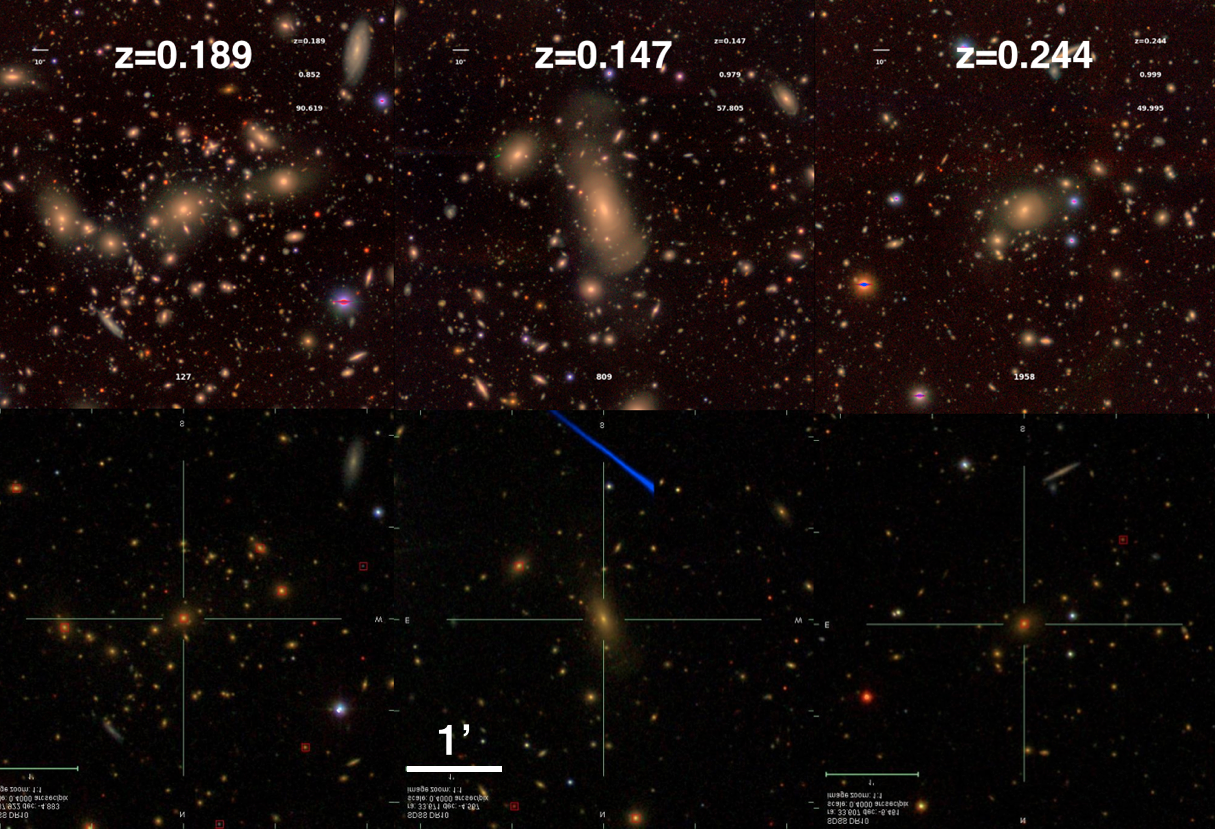
\includegraphics[width=15.5cm]{fig/redbcg_color.png}
    \caption{\todo{Remake this figure}: Comparison of RGB 3-color images 
    of nearby massive elliptical galaxies using SDSS and HSC images.  
    The images are generated using $gri$ band images according to the algorithm 
    of \citep{Lupton2004} with arcsinh stretch.  
    It is clear that the depth of HSC image help map the stellar distributions 
    out to much larger radius, and revel more details in the outskirts compared 
    to the SDSS ones.}\label{figure:1}
\end{figure}

% Fig. 2
\clearpage
\figurenum{2}
\begin{figure}
    \centering 
    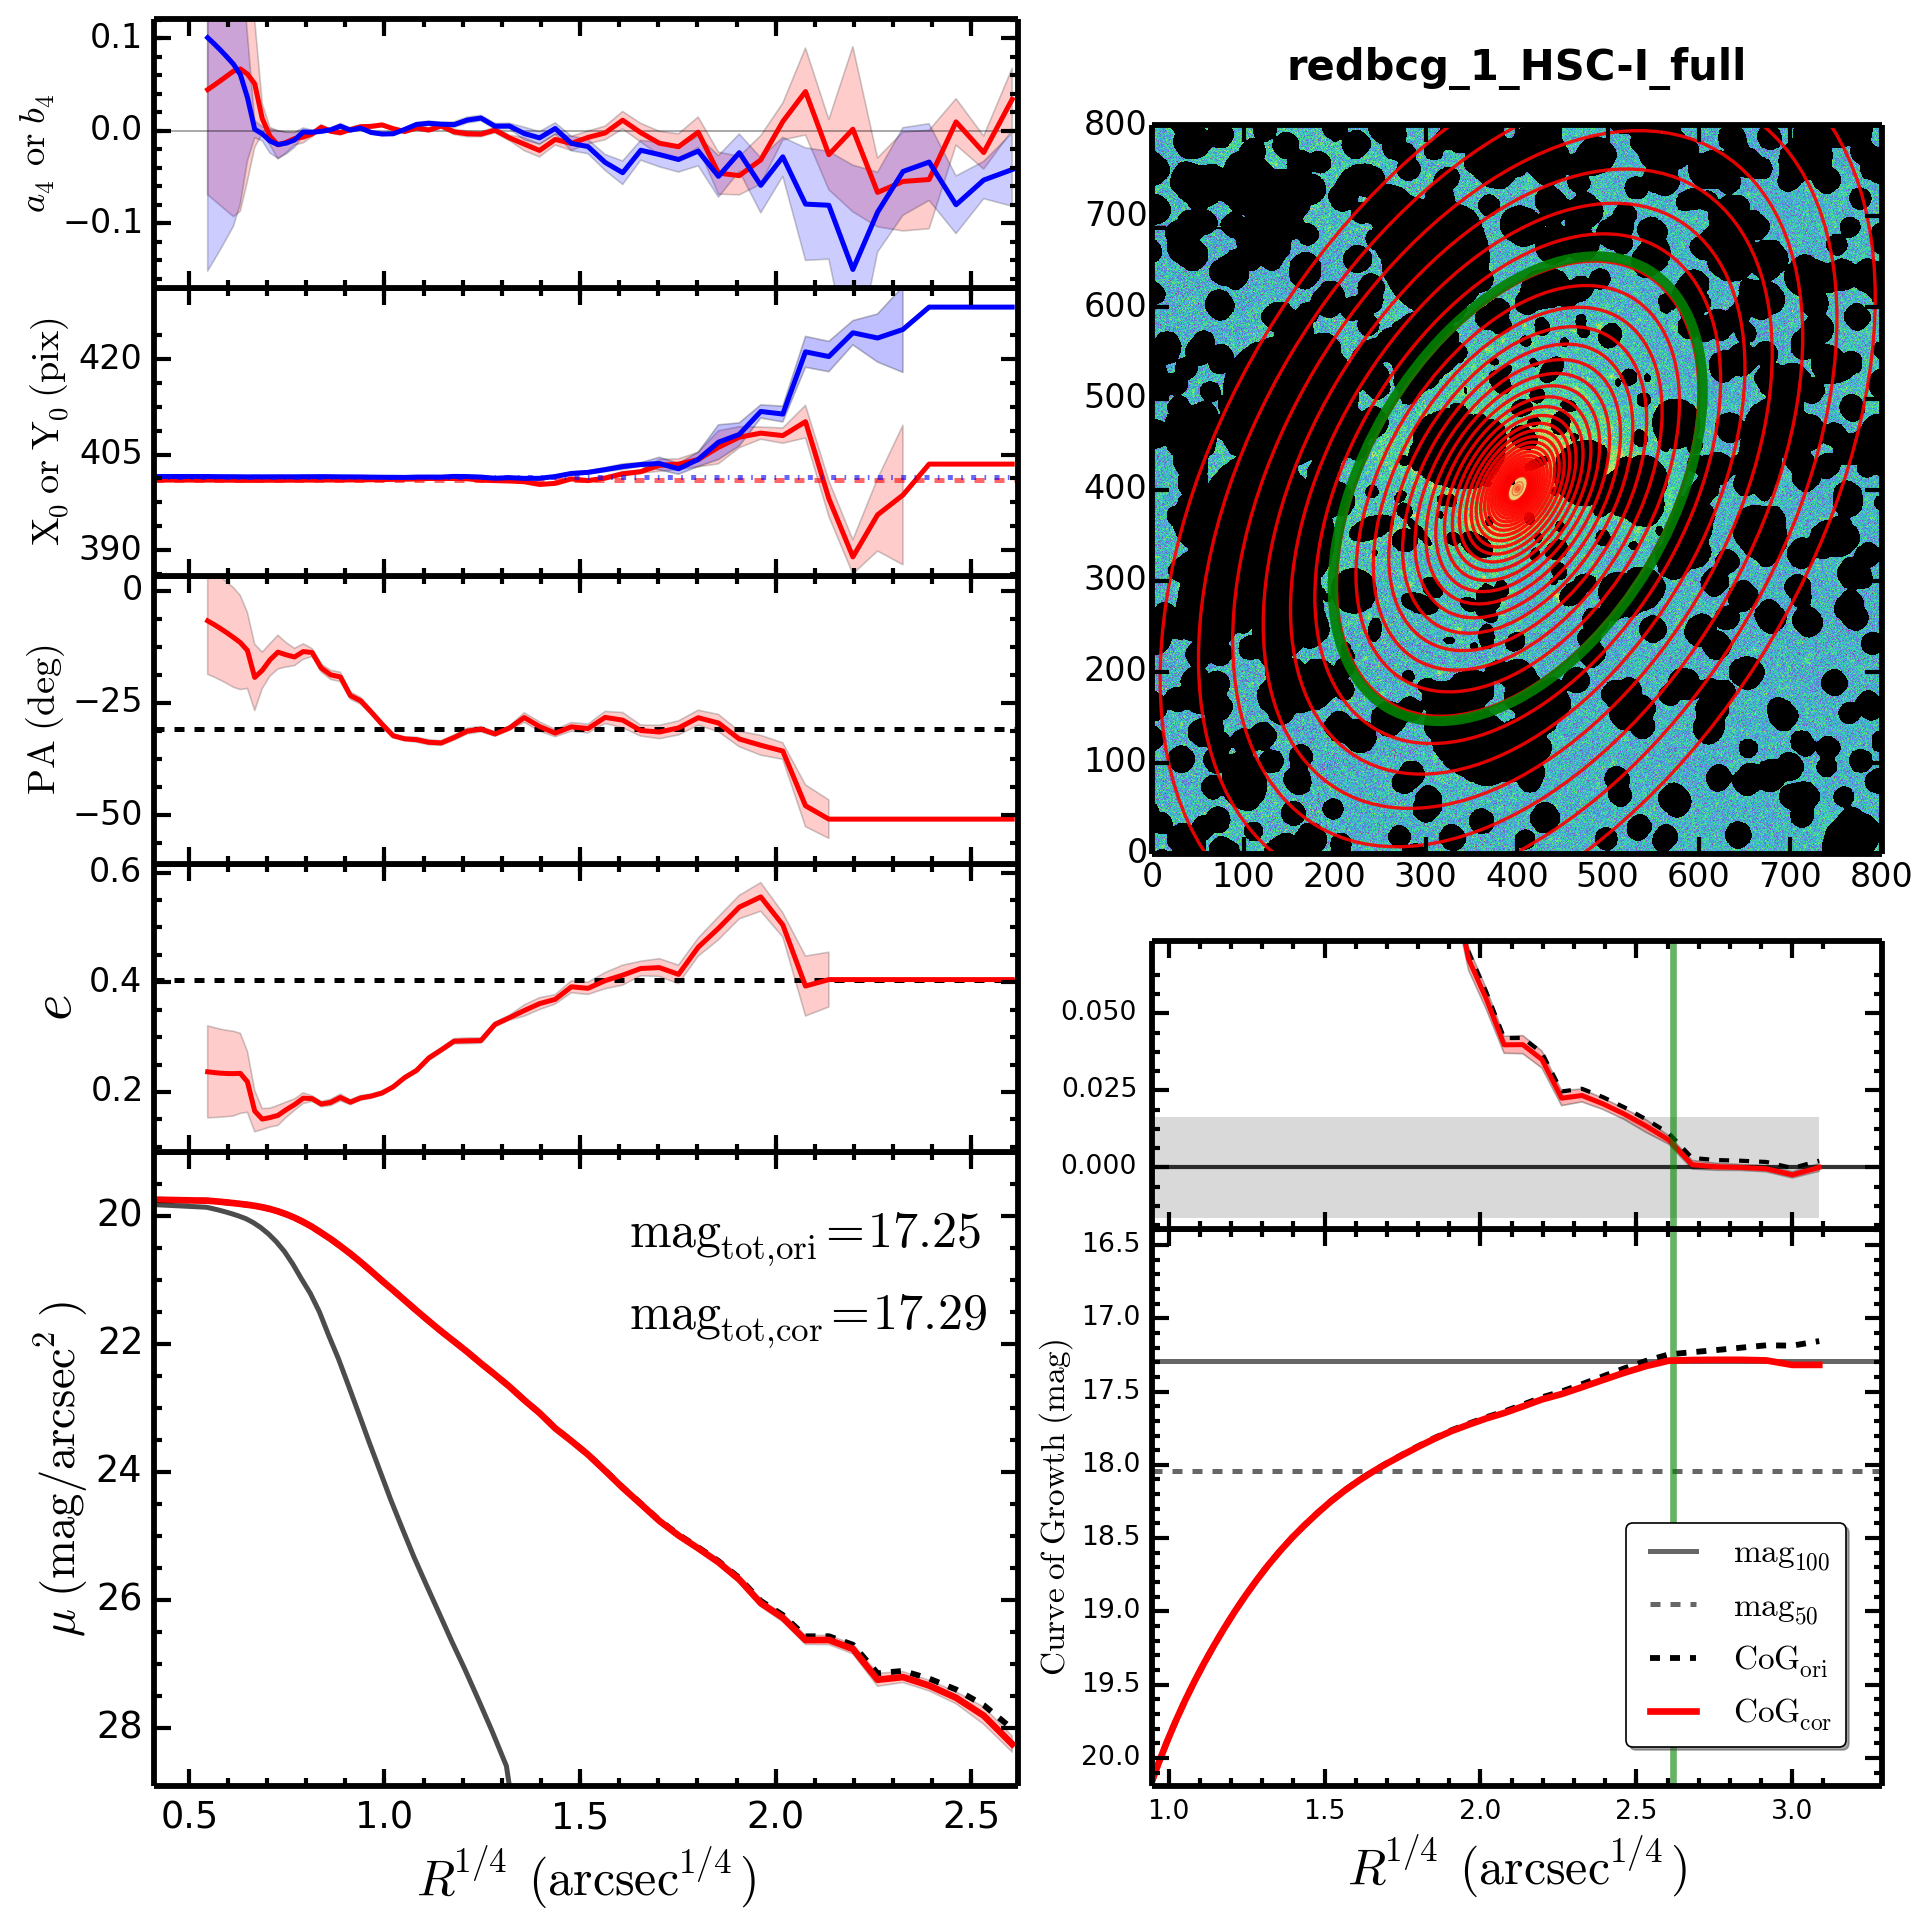
\includegraphics[width=15.5cm]{fig/redbcg_ellipse_example.png}
    \caption{Figure.2\todo{Caption}}\label{figure:2}
\end{figure}

% Fig. 3
\clearpage
\figurenum{3}
\begin{figure}
    \centering 
    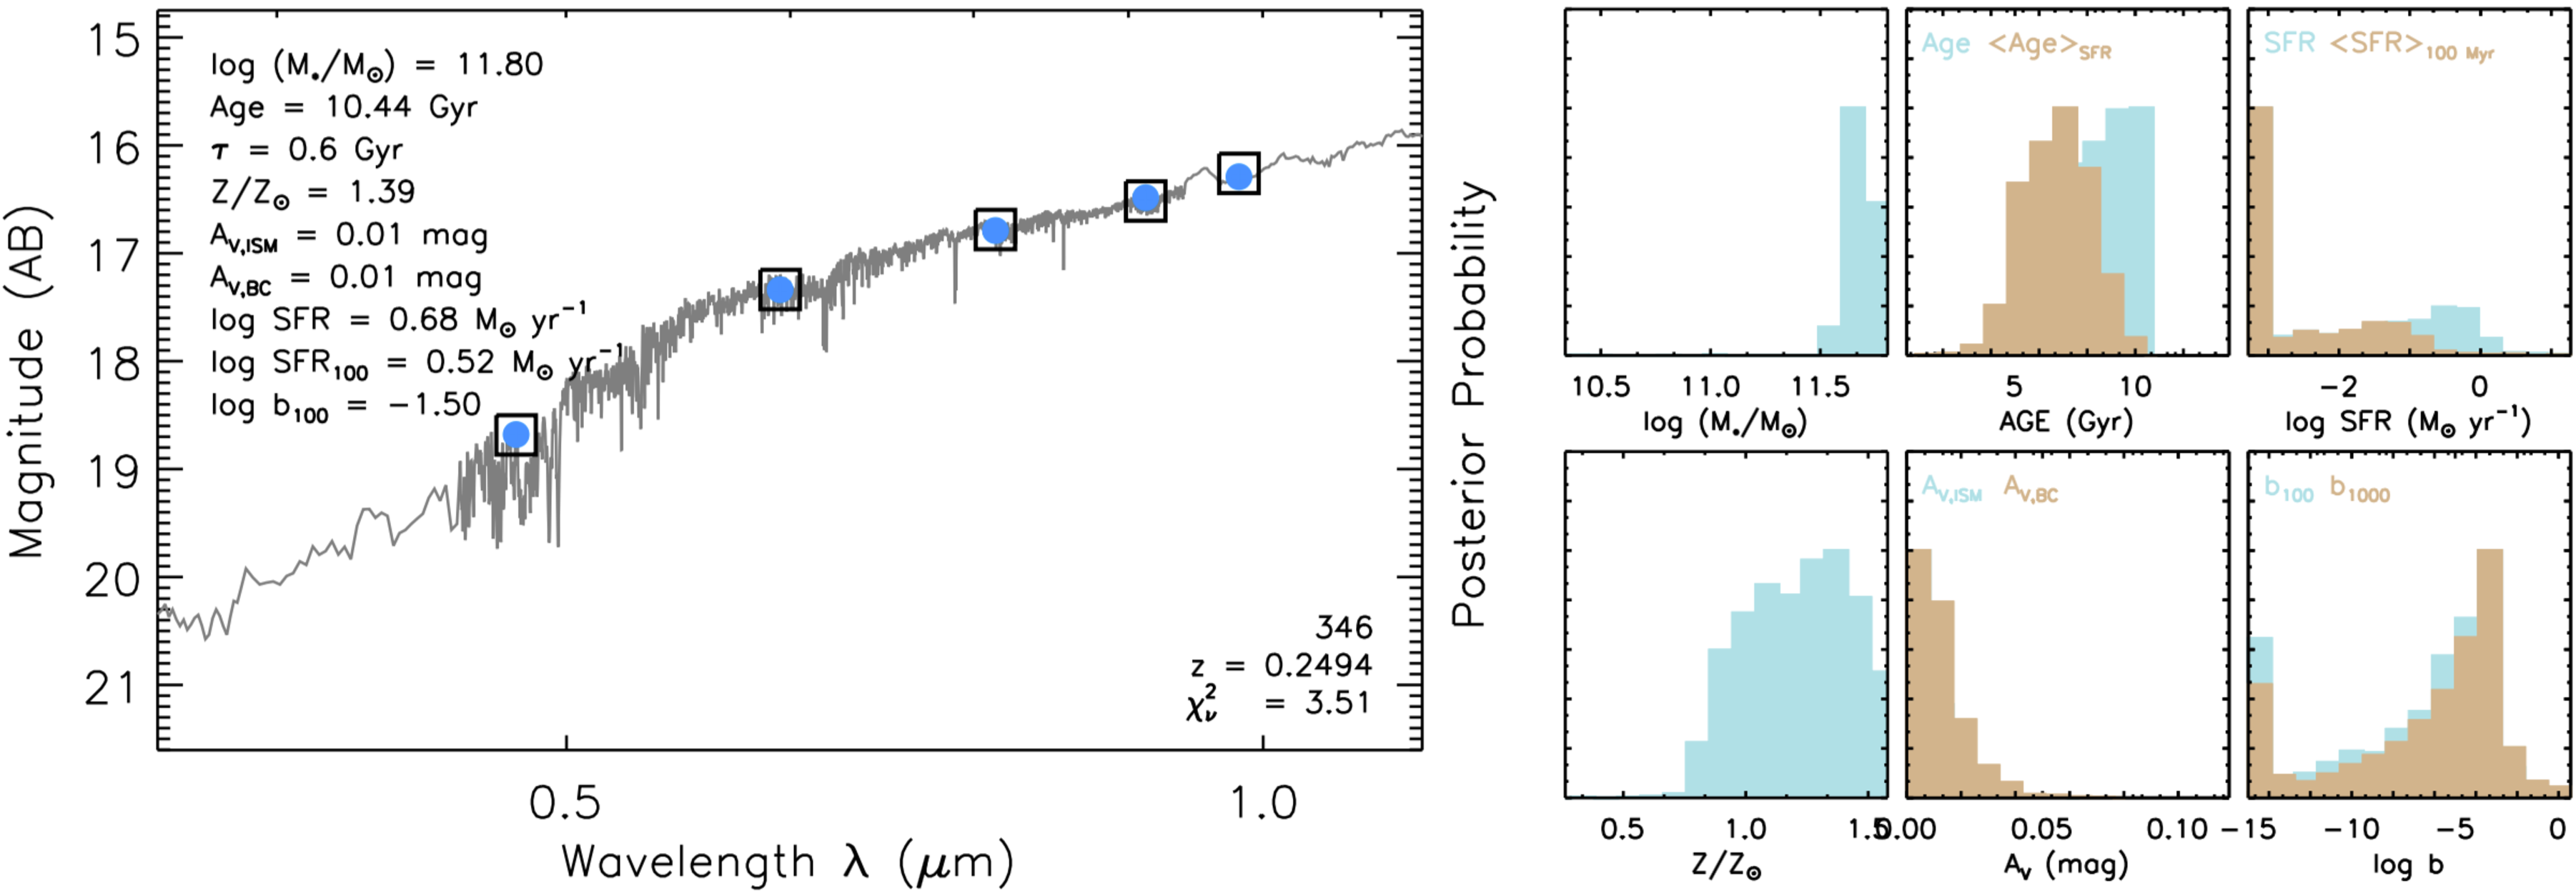
\includegraphics[width=10.5cm]{fig/redbcg_isedfit_example}
    \caption{Figure.3\todo{Caption}}\label{figure:3}
\end{figure}

% Fig. 4
\clearpage
\figurenum{4}
\begin{figure}
    \centering 
    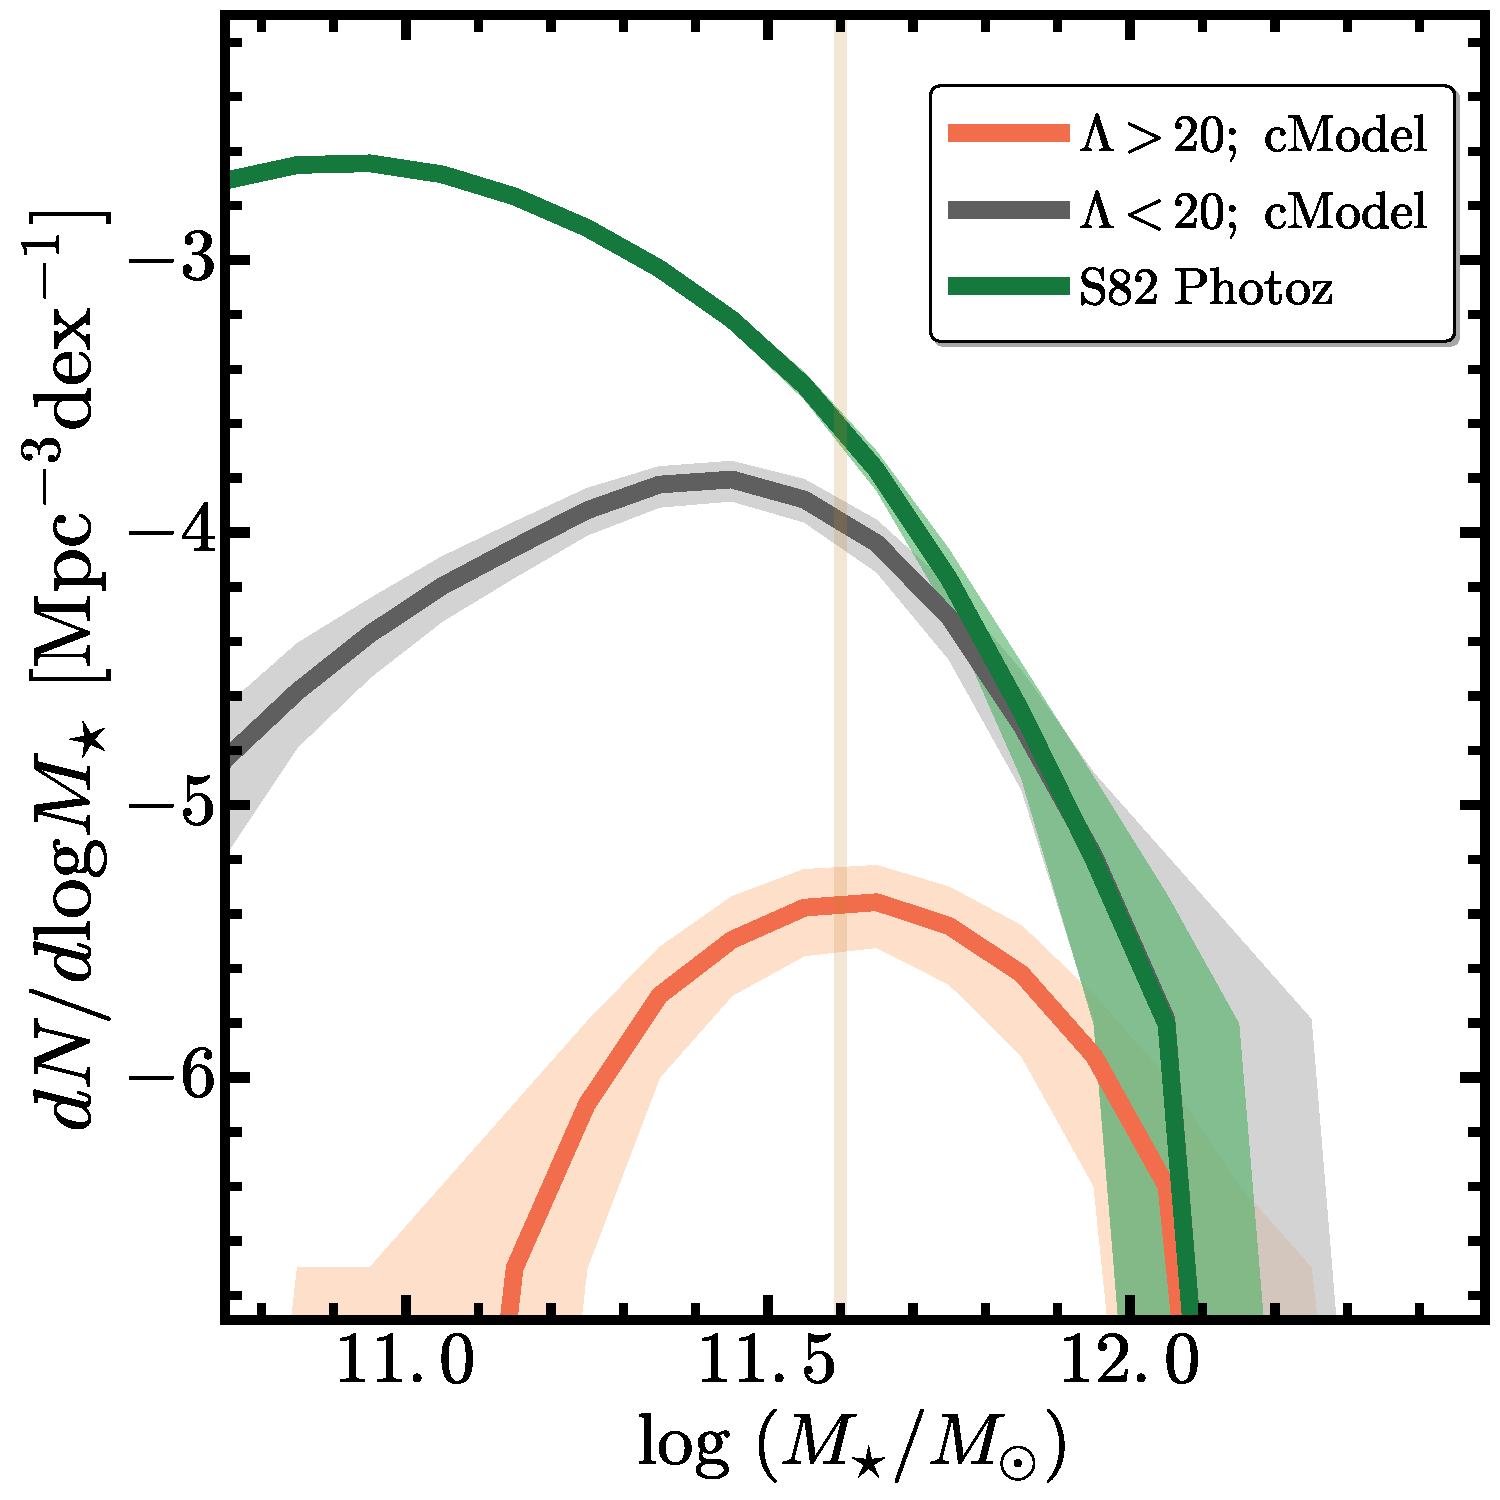
\includegraphics[width=14.5cm]{fig/redbcg_hsc_s82}
    \caption{Figure.4\todo{Caption}}\label{figure:4}
\end{figure}

% Fig. 5
\clearpage
\figurenum{5}
\begin{figure}
    \centering 
    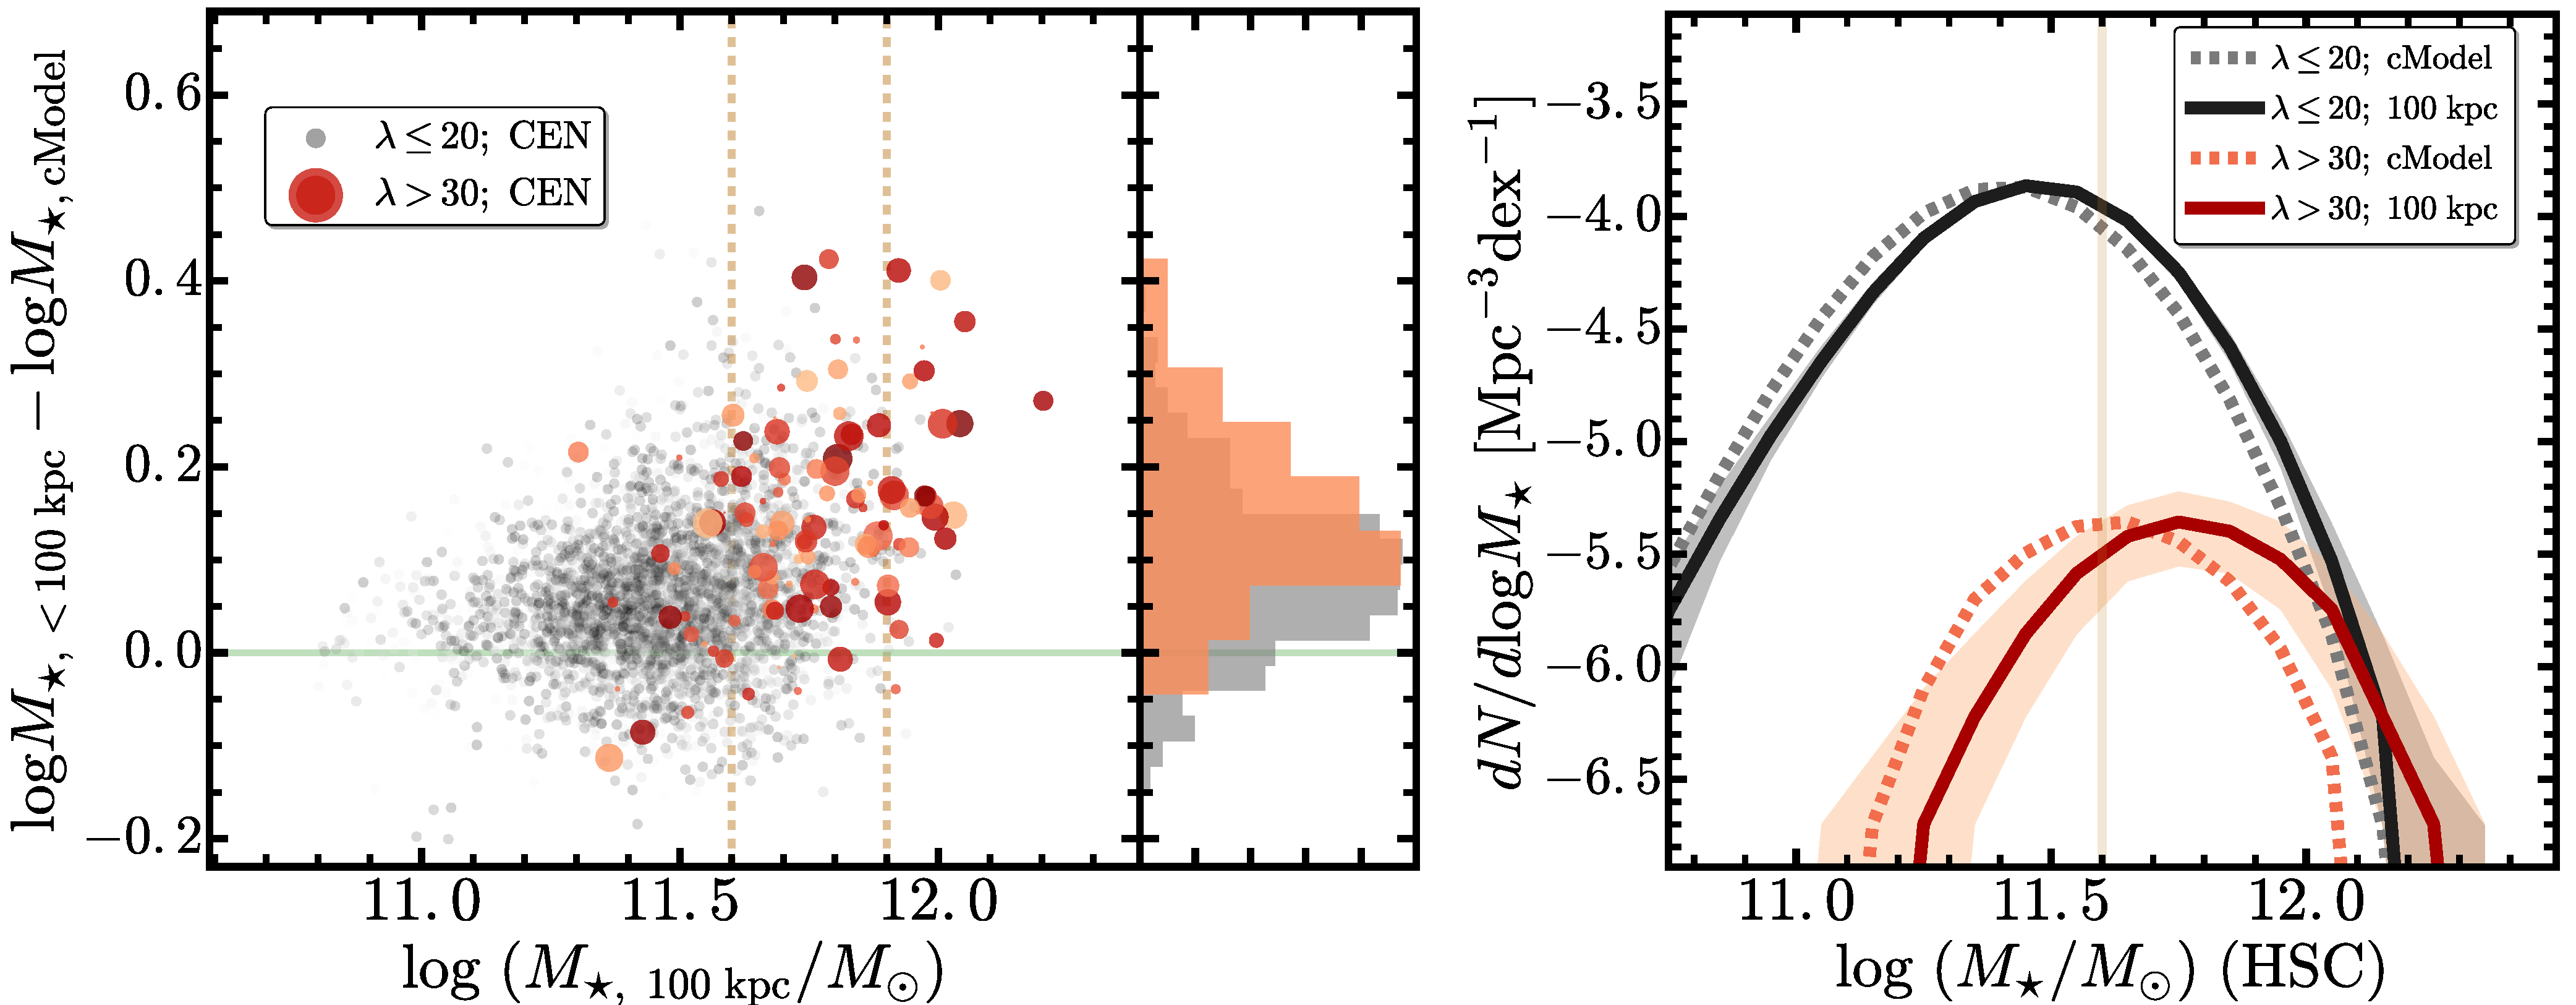
\includegraphics[width=18.5cm]{fig/redbcg_lf_smf}
    \caption{Figure.5\todo{Caption}}\label{figure:5}
\end{figure}

% Fig. 6
\clearpage
\figurenum{6}
\begin{figure}
    \centering 
    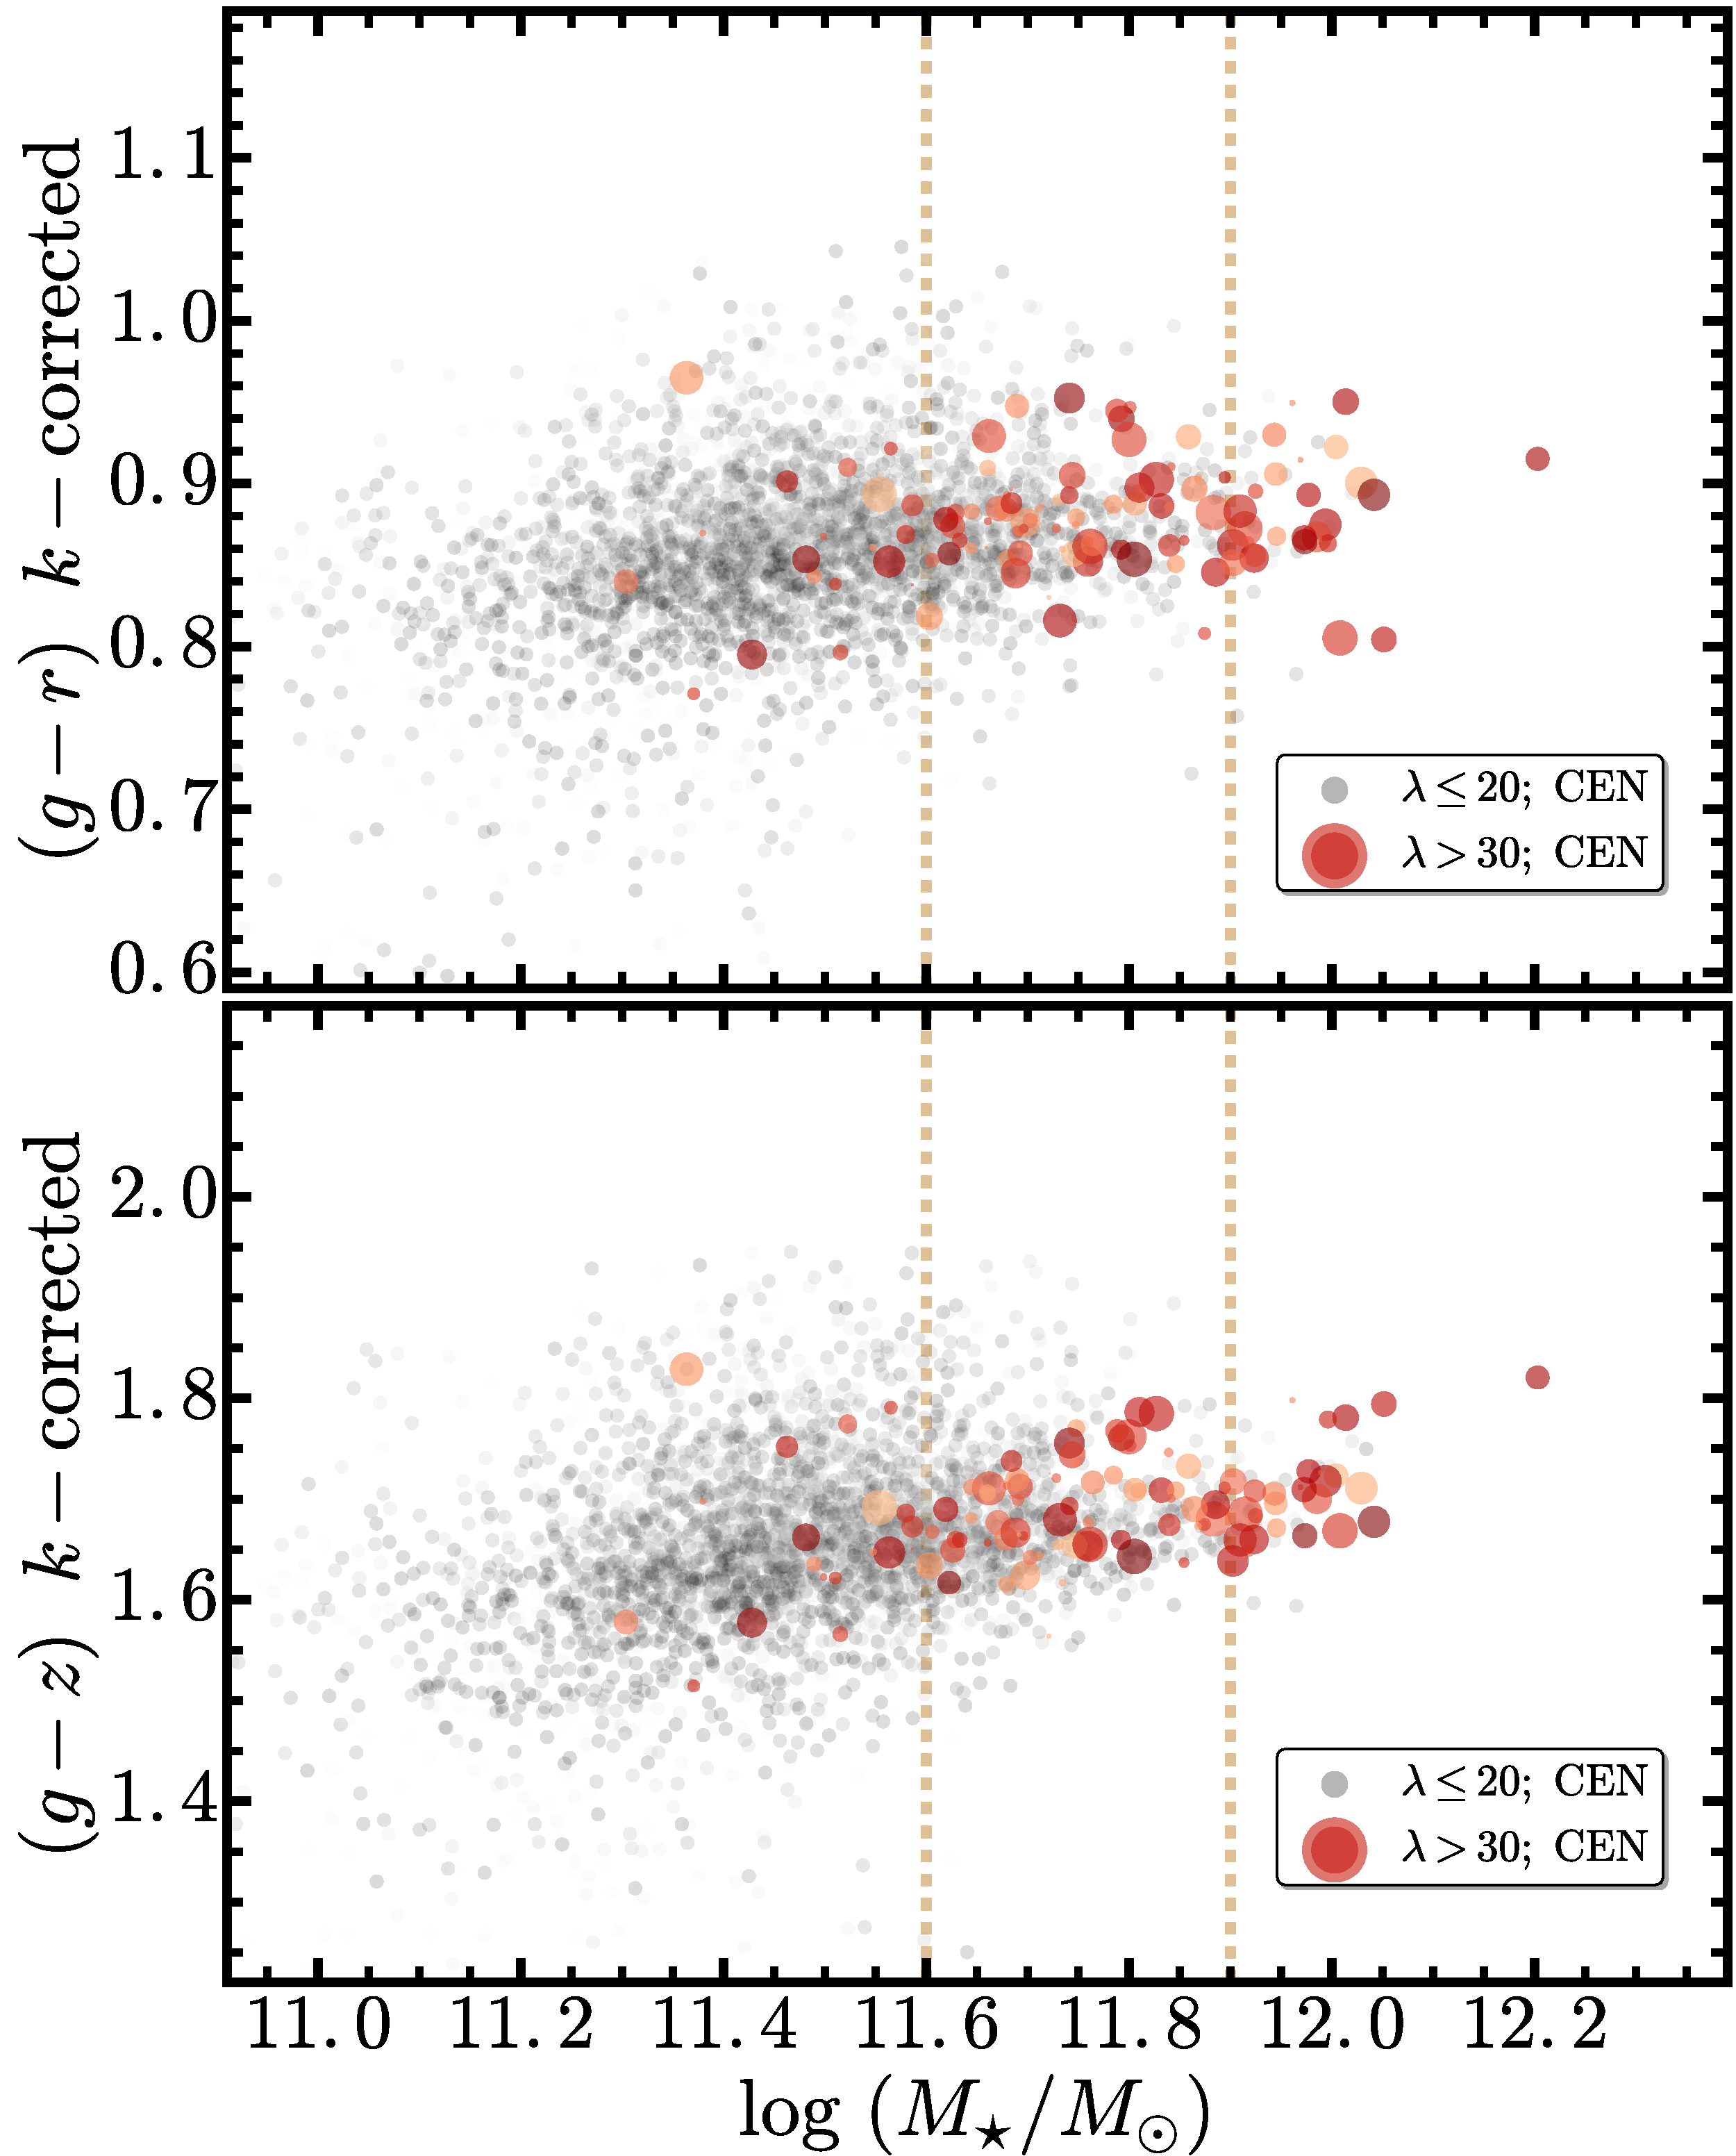
\includegraphics[width=12.5cm]{fig/redbcg_mass_color}
    \caption{Figure.6\todo{Caption}}\label{figure:6}
\end{figure}

% Fig. 7
\clearpage
\figurenum{7}
\begin{figure}
    \centering 
    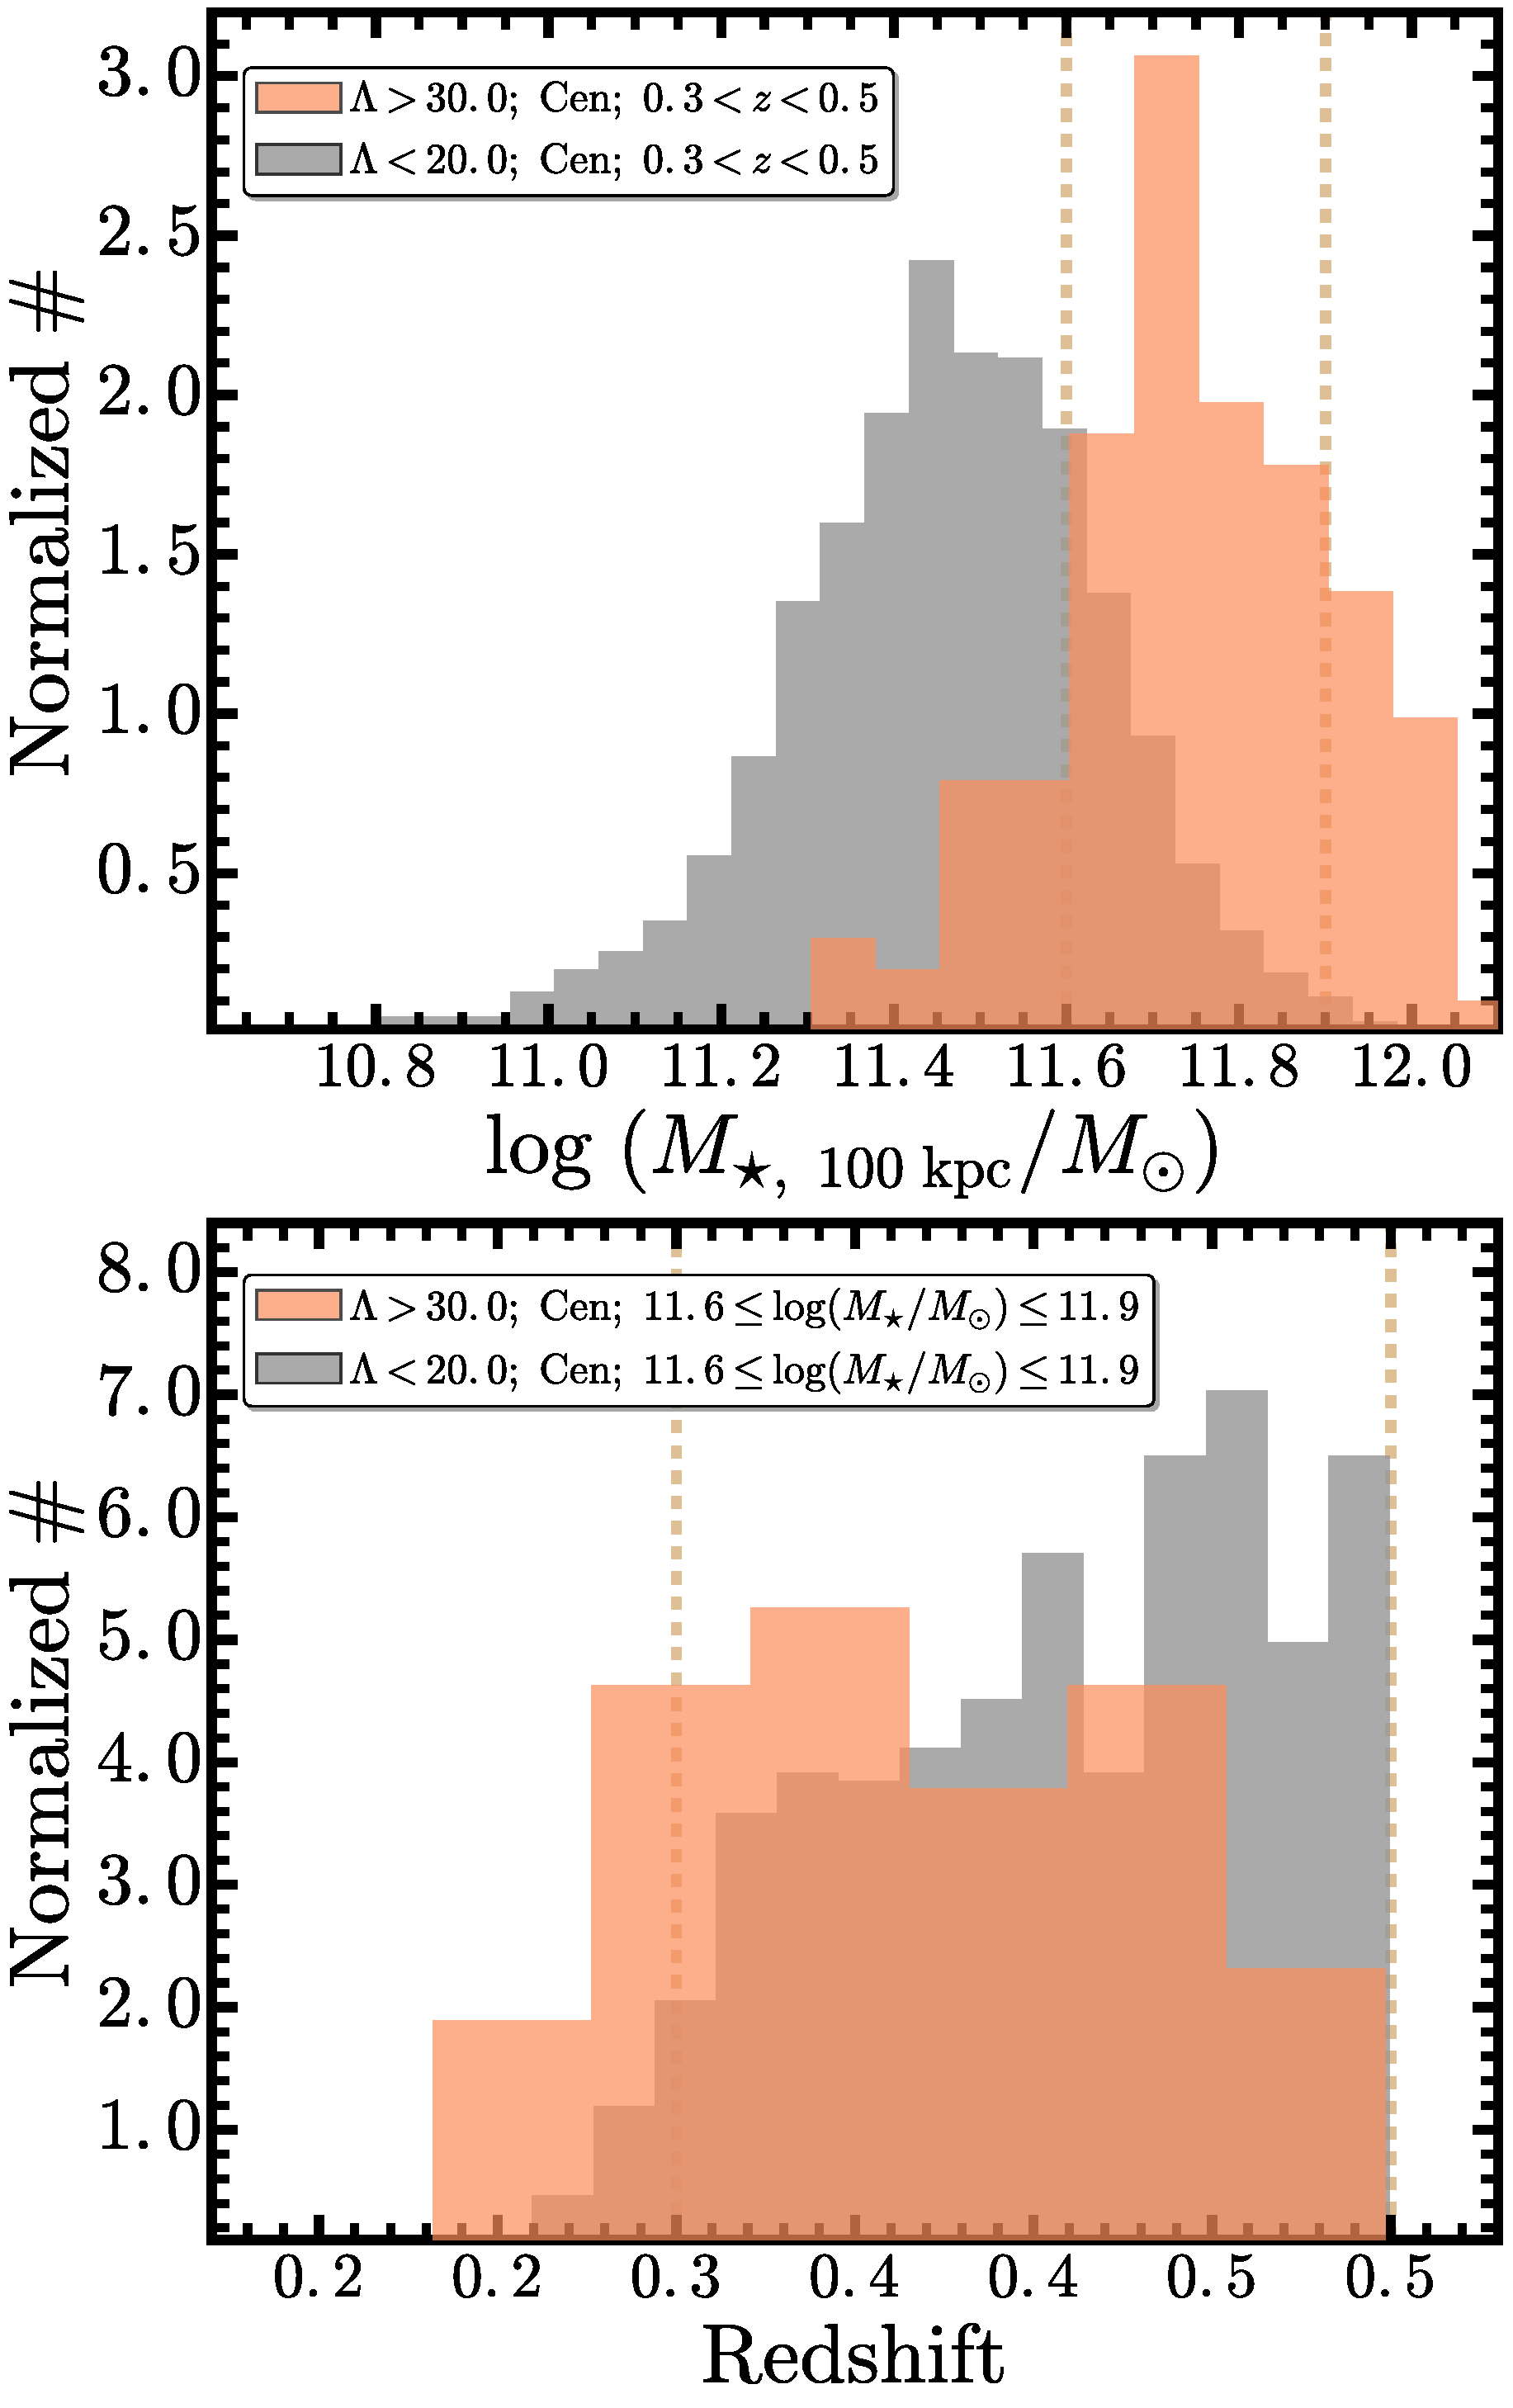
\includegraphics[width=12.5cm]{fig/redbcg_mass_z_hist}
    \caption{Figure.7\todo{Caption}}\label{figure:7}
\end{figure}

% Fig. 8
\clearpage
\figurenum{8}
\begin{figure}
    \centering 
    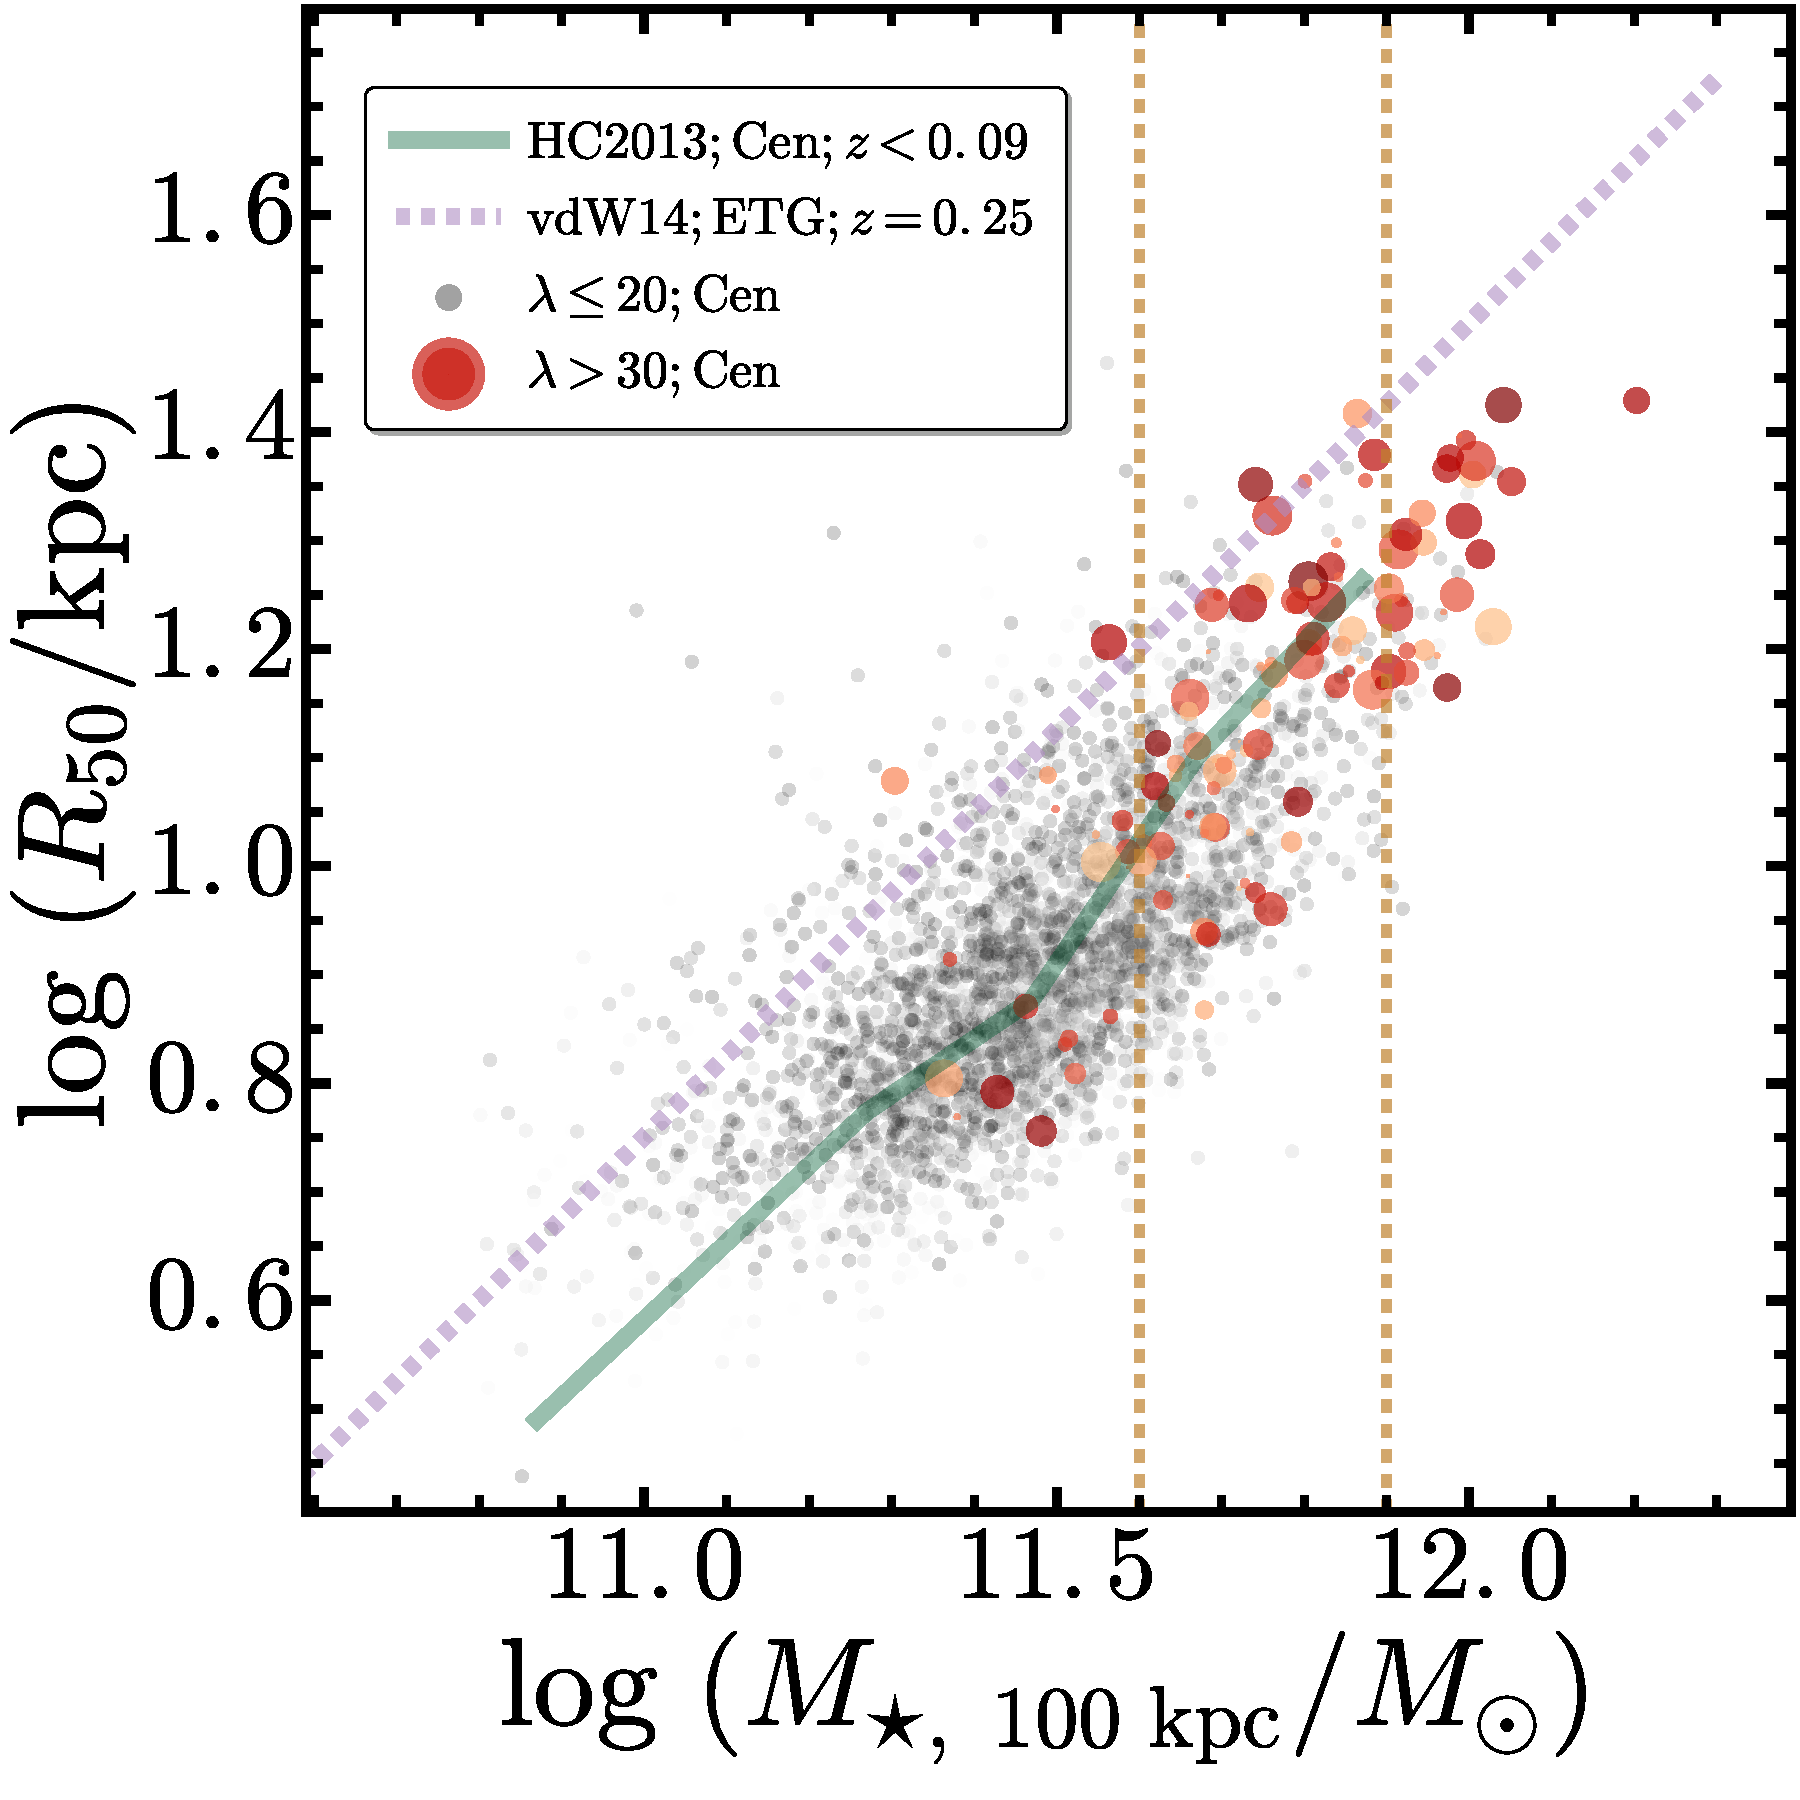
\includegraphics[width=14.0cm]{fig/redbcg_mass_r50}
    \caption{Figure.8\todo{Caption}}\label{figure:8}
\end{figure}

% Fig. 9
\clearpage
\figurenum{9}
\begin{figure}
    \centering 
    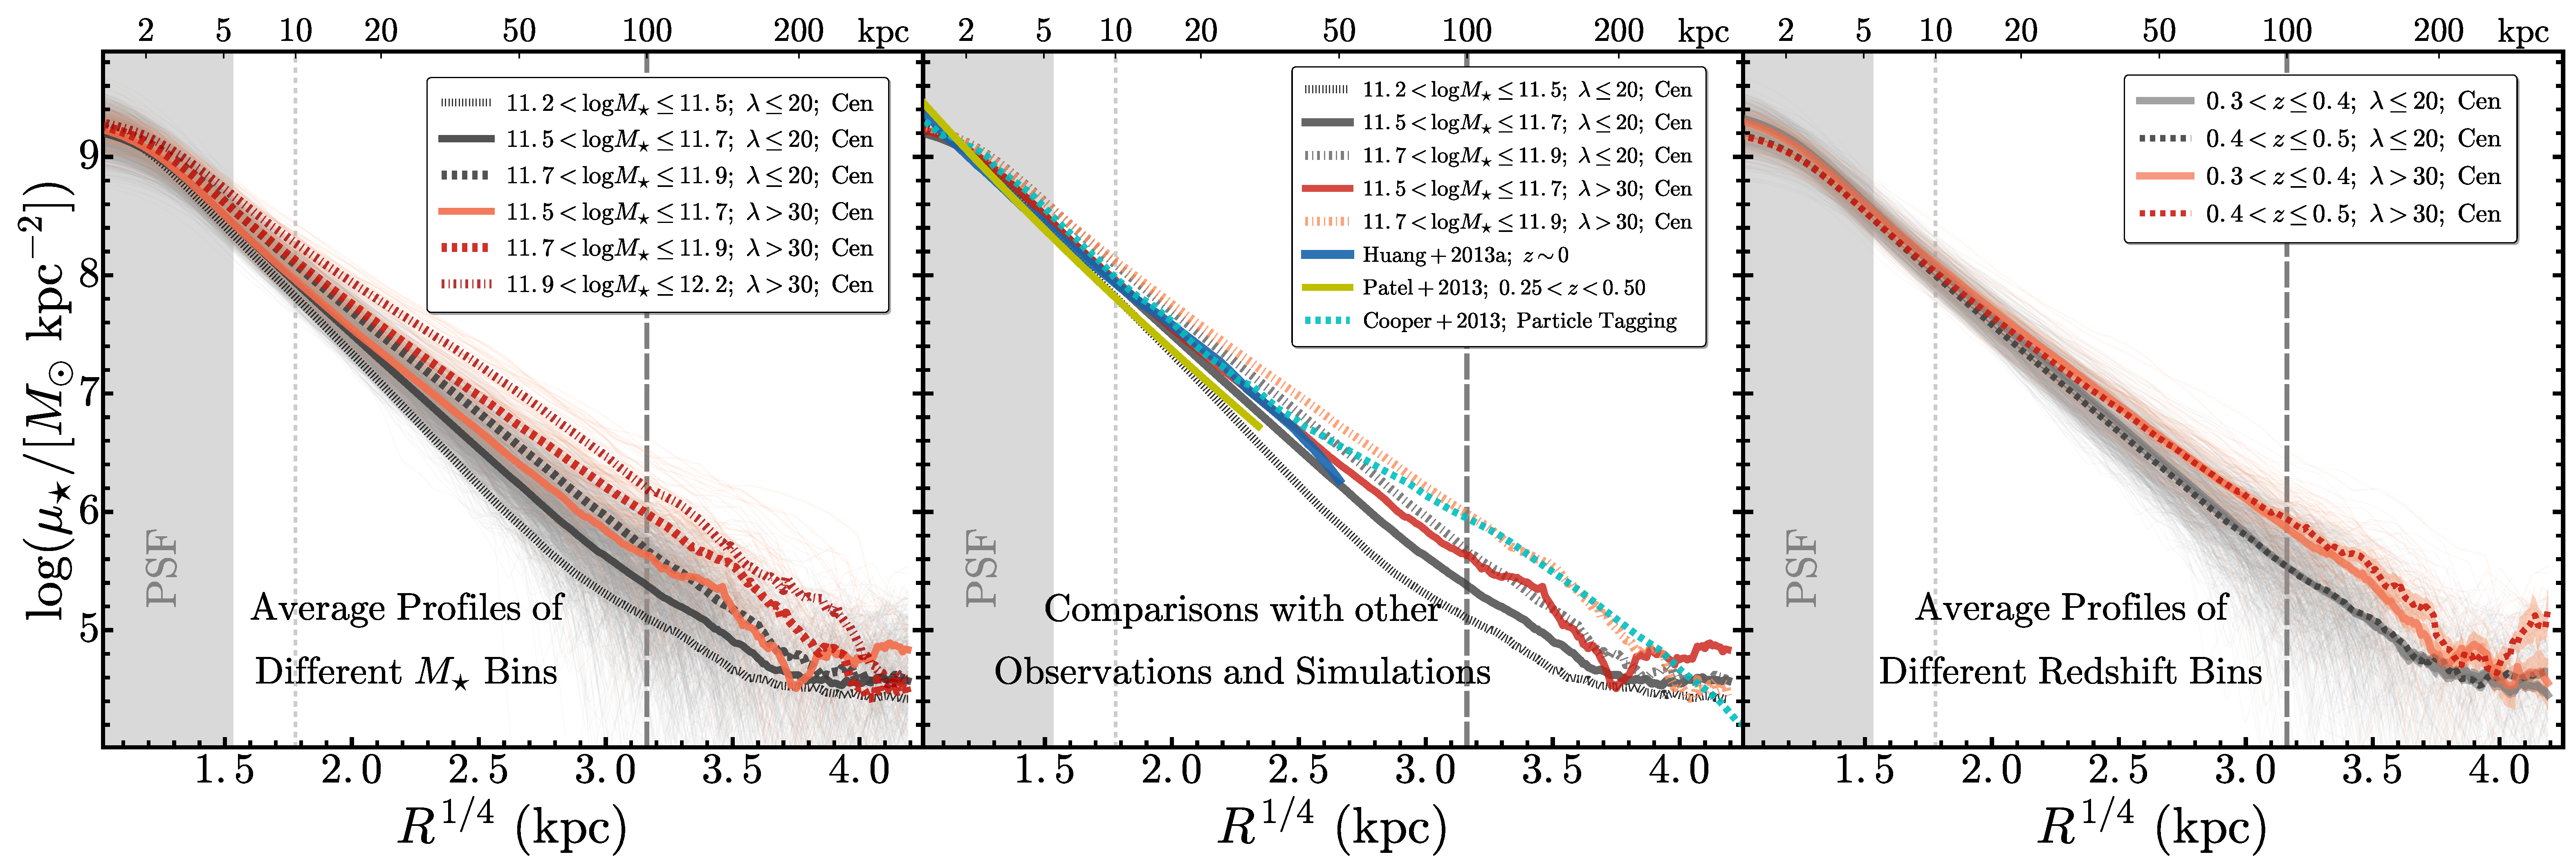
\includegraphics[width=18.5cm]{fig/redbcg_avg_prof}
    \caption{Figure.9\todo{Caption}}\label{figure:9}
\end{figure}

% Fig. 10
\clearpage
\figurenum{10}
\begin{figure}
    \centering 
    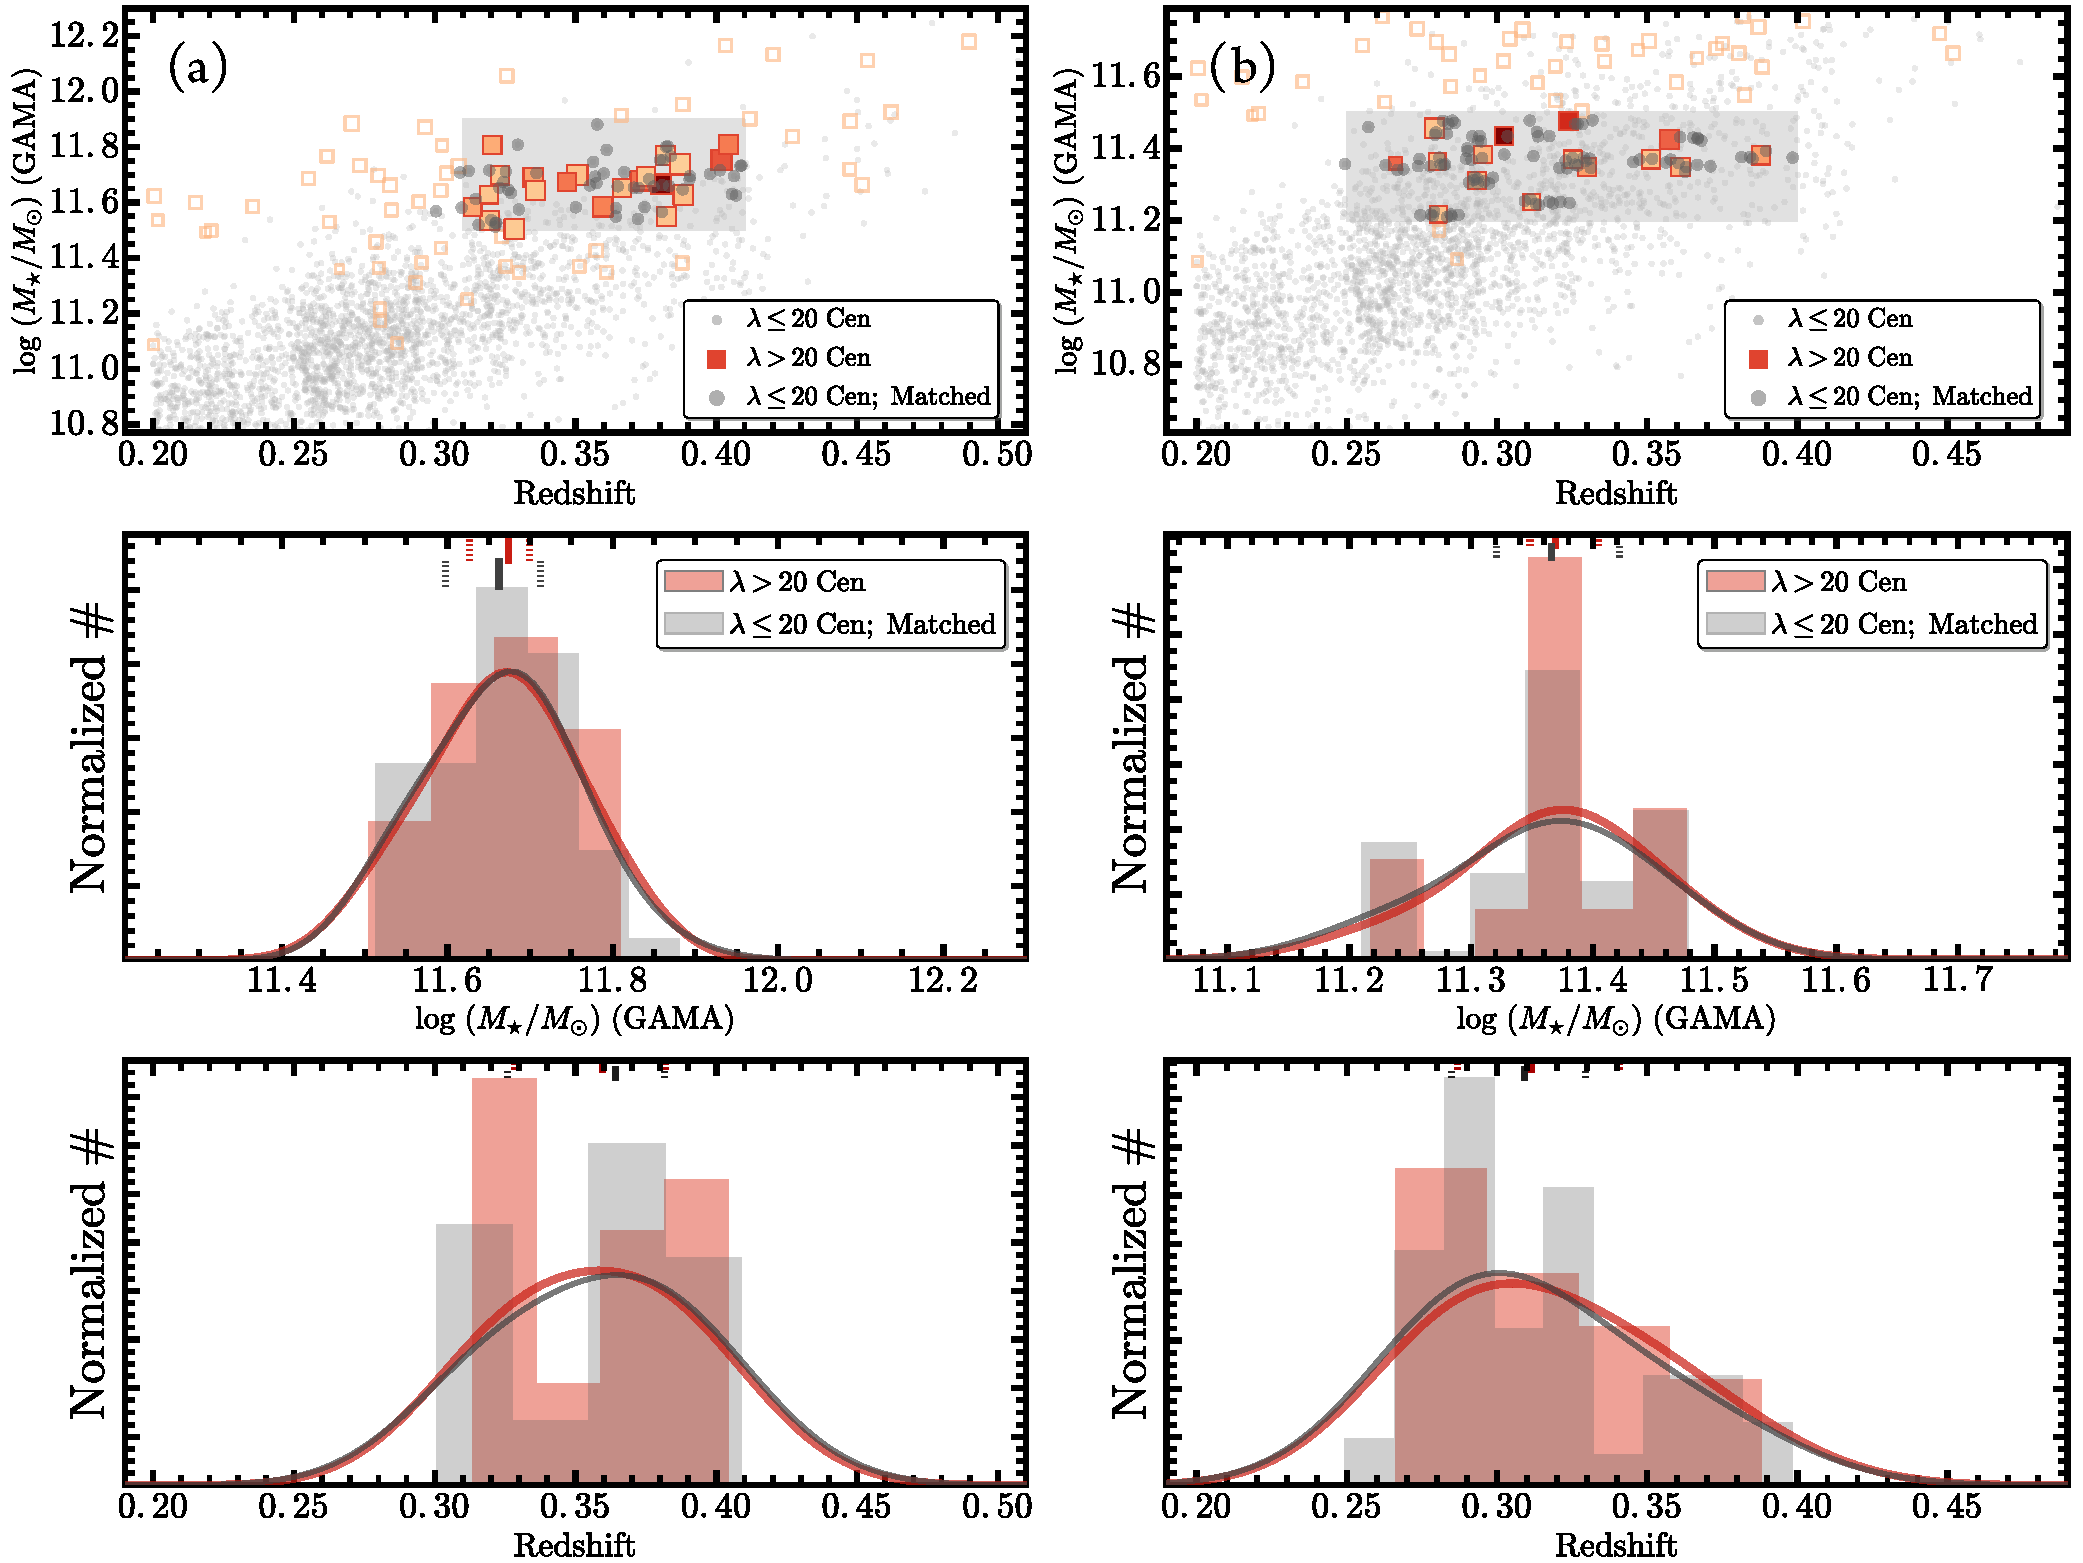
\includegraphics[width=16.0cm]{fig/redbcg_prof_gama_1}
    \caption{Figure.10\todo{Caption}}\label{figure:10}
\end{figure}

% Fig. 11
\clearpage
\figurenum{11}
\begin{figure}
    \centering 
    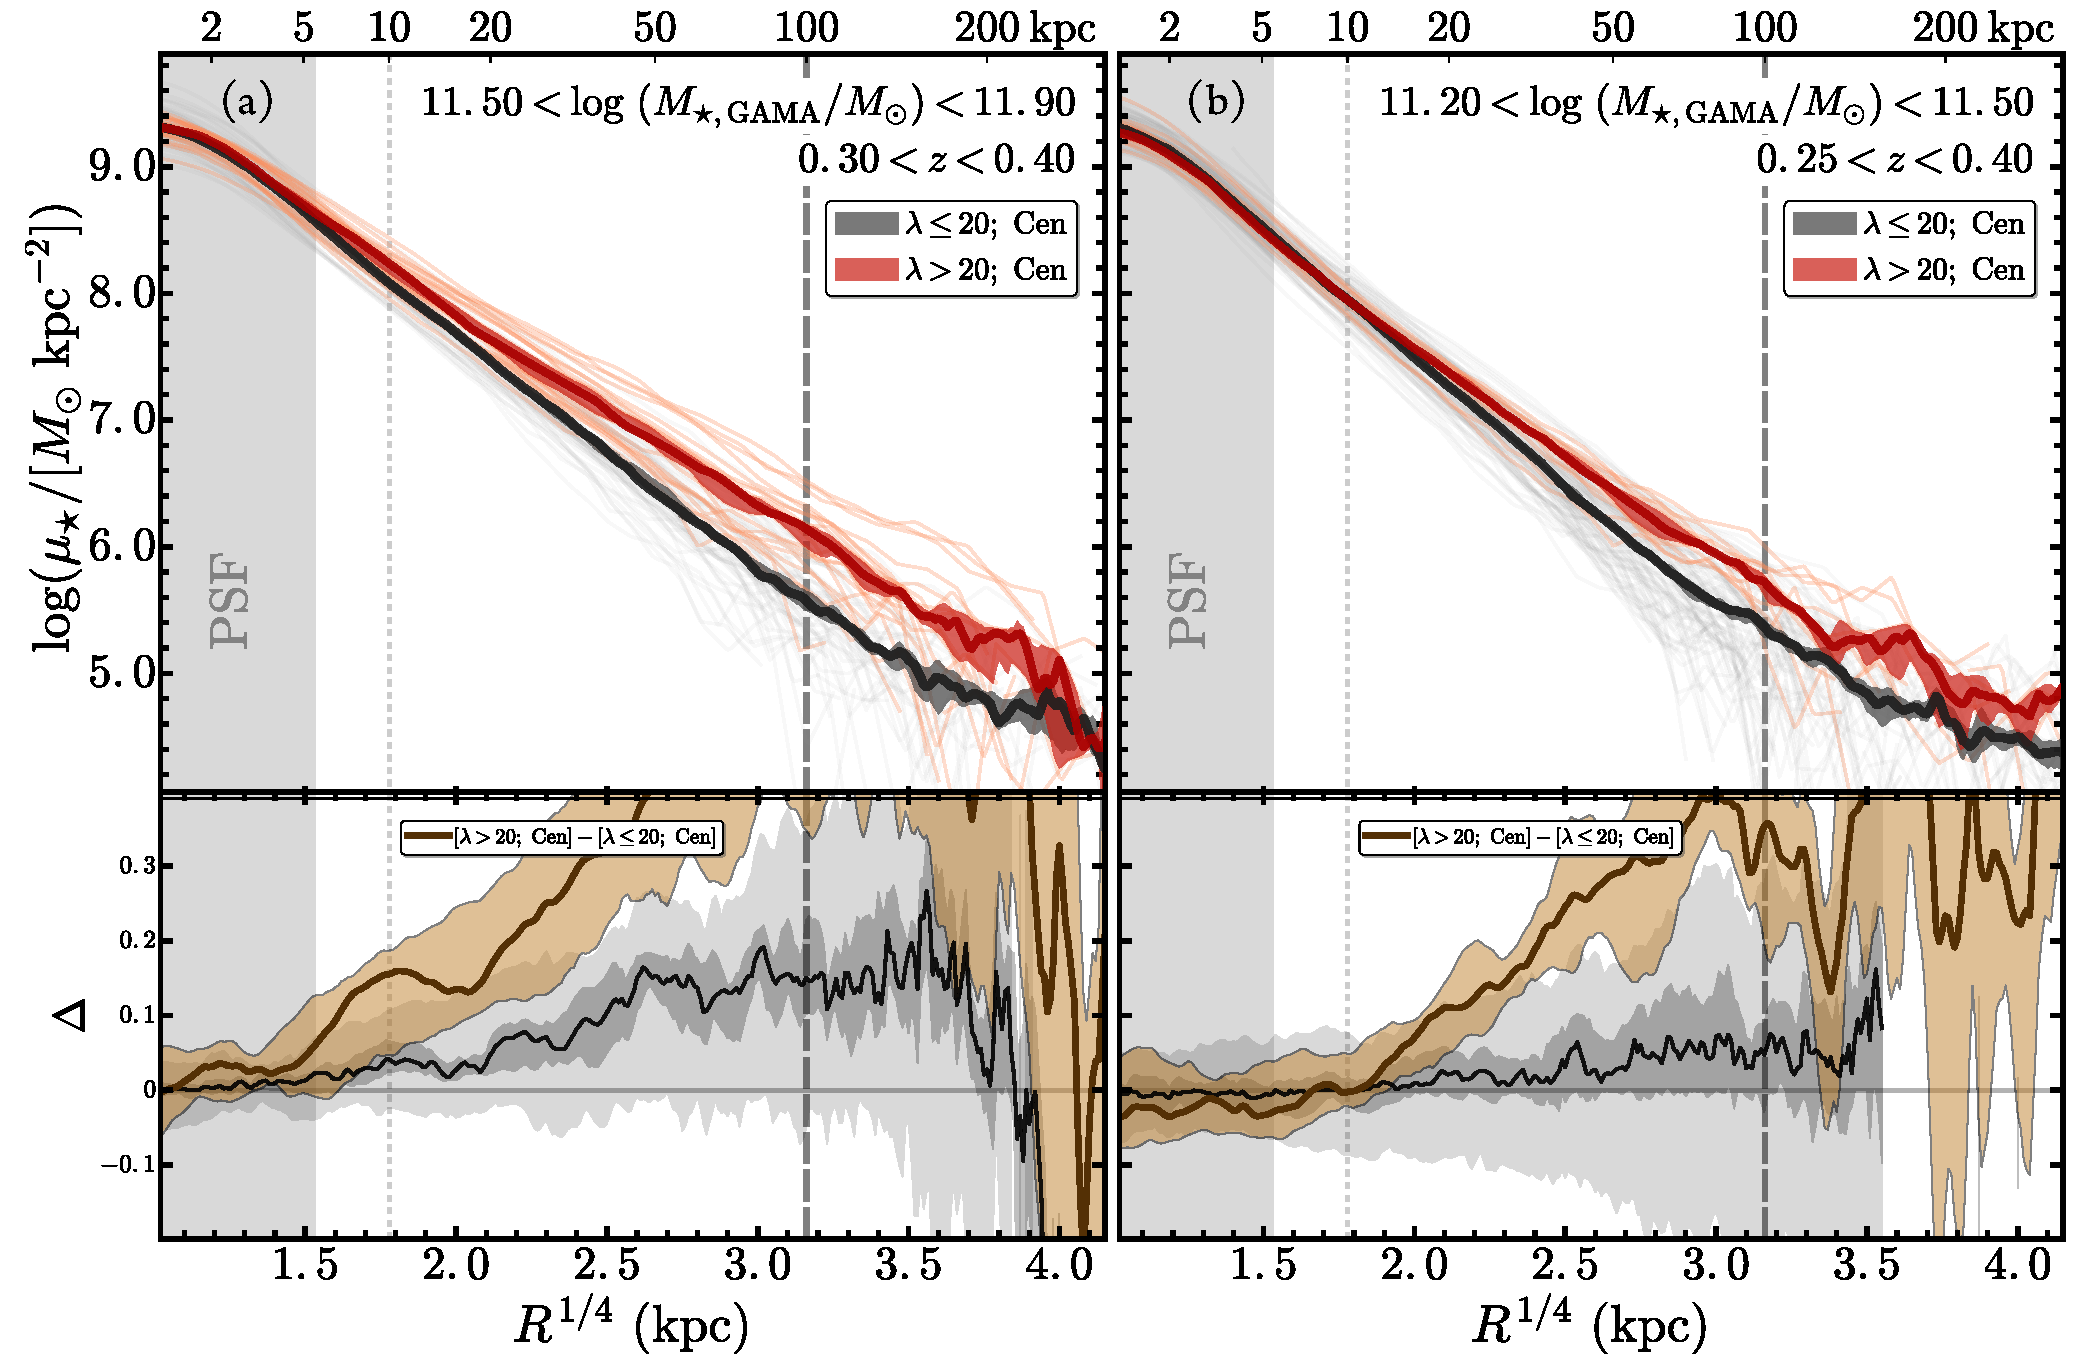
\includegraphics[width=18.0cm]{fig/redbcg_prof_gama_2}
    \caption{Figure.11\todo{Caption}}\label{figure:11}
\end{figure}

% Fig. A1
\clearpage
\figurenum{A1}
\begin{figure}
    \centering 
    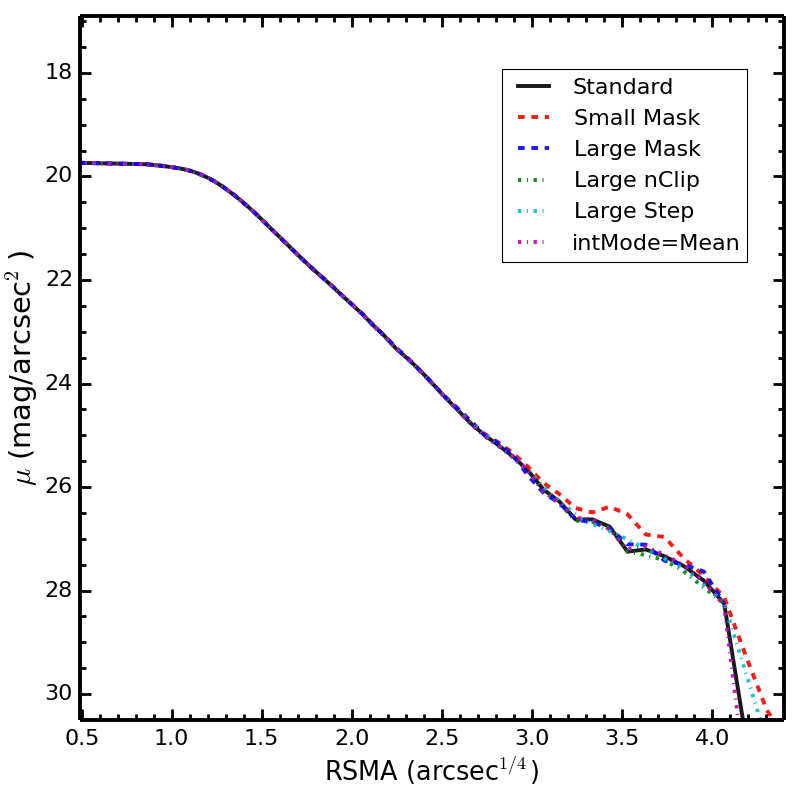
\includegraphics[width=14.0cm]{fig/redbcg_1_HSC-I_full_imgsub_ellip_default_compare.png}
    \caption{Figure.A1\todo{Caption}}\label{figure:A1}
\end{figure}

% Fig. B1
\clearpage
\figurenum{2a}
\begin{figure}
    \centering 
    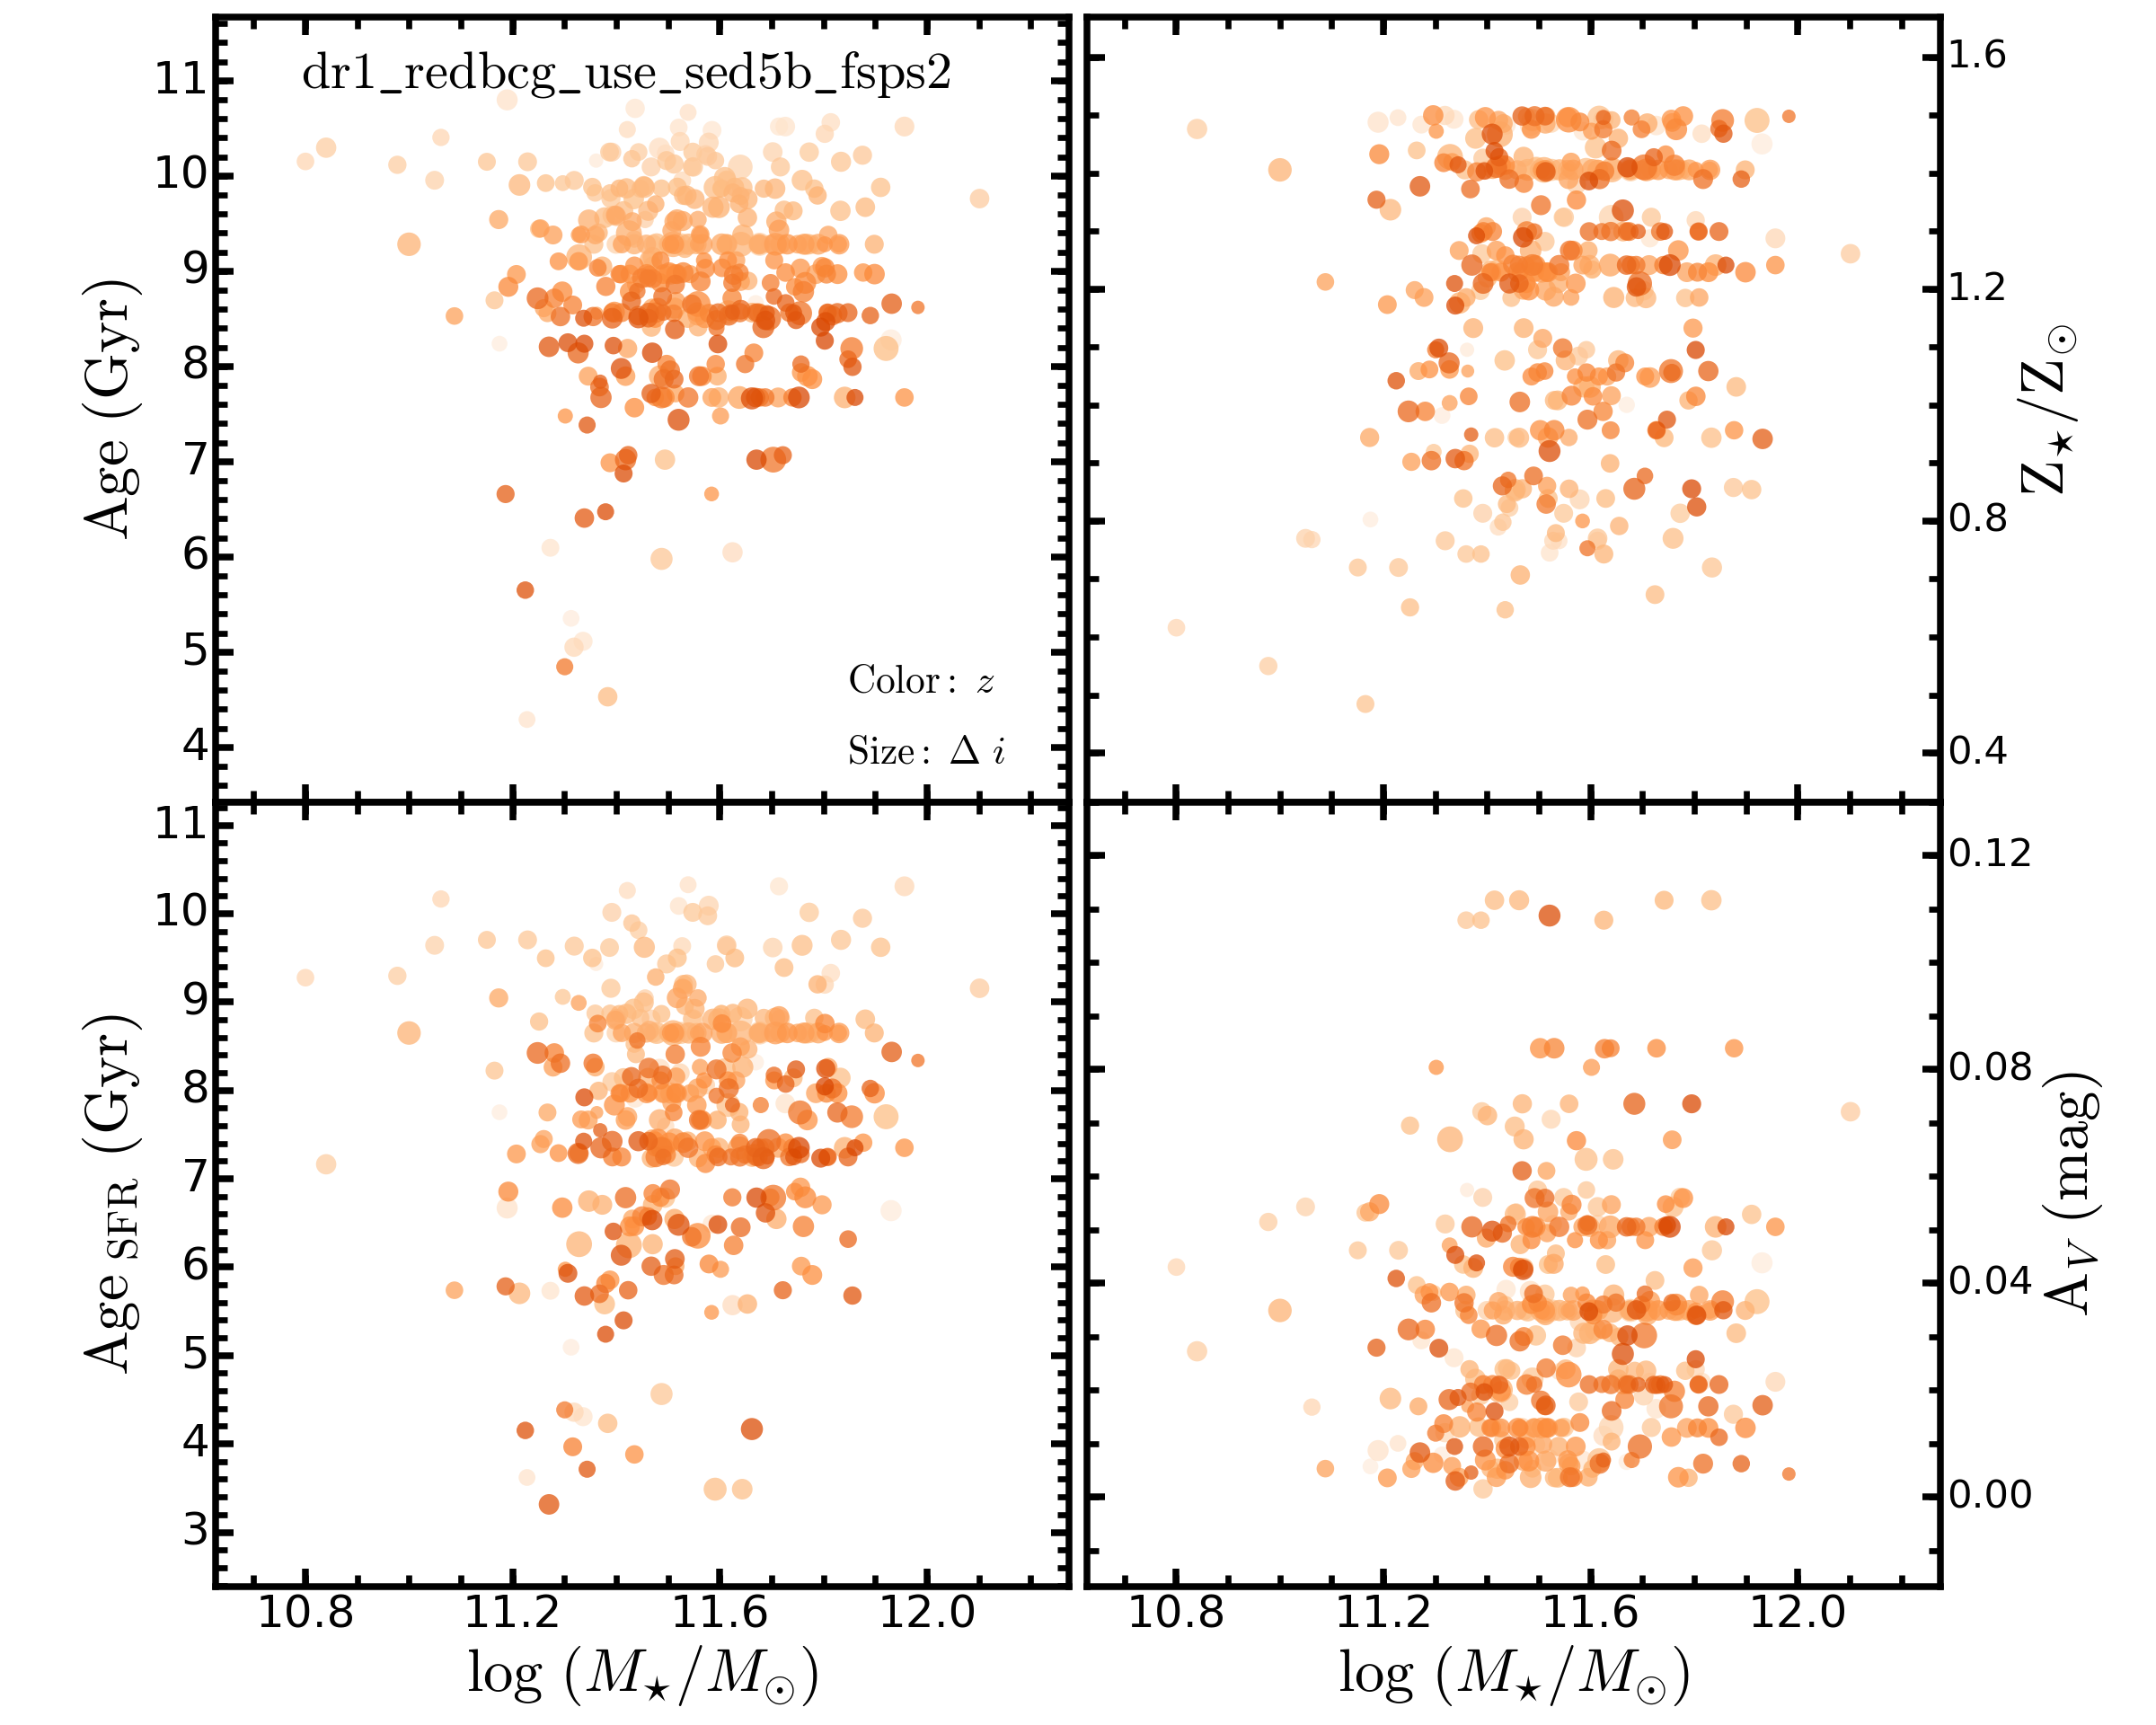
\includegraphics[width=11.5cm]{fig/dr1_redbcg_use_sed5b_fsps2_logm_plots}
    \caption{Figure.2a\todo{Caption}}\label{figure:2a}
\end{figure}

\figurenum{2b}
\begin{figure}
    \centering 
    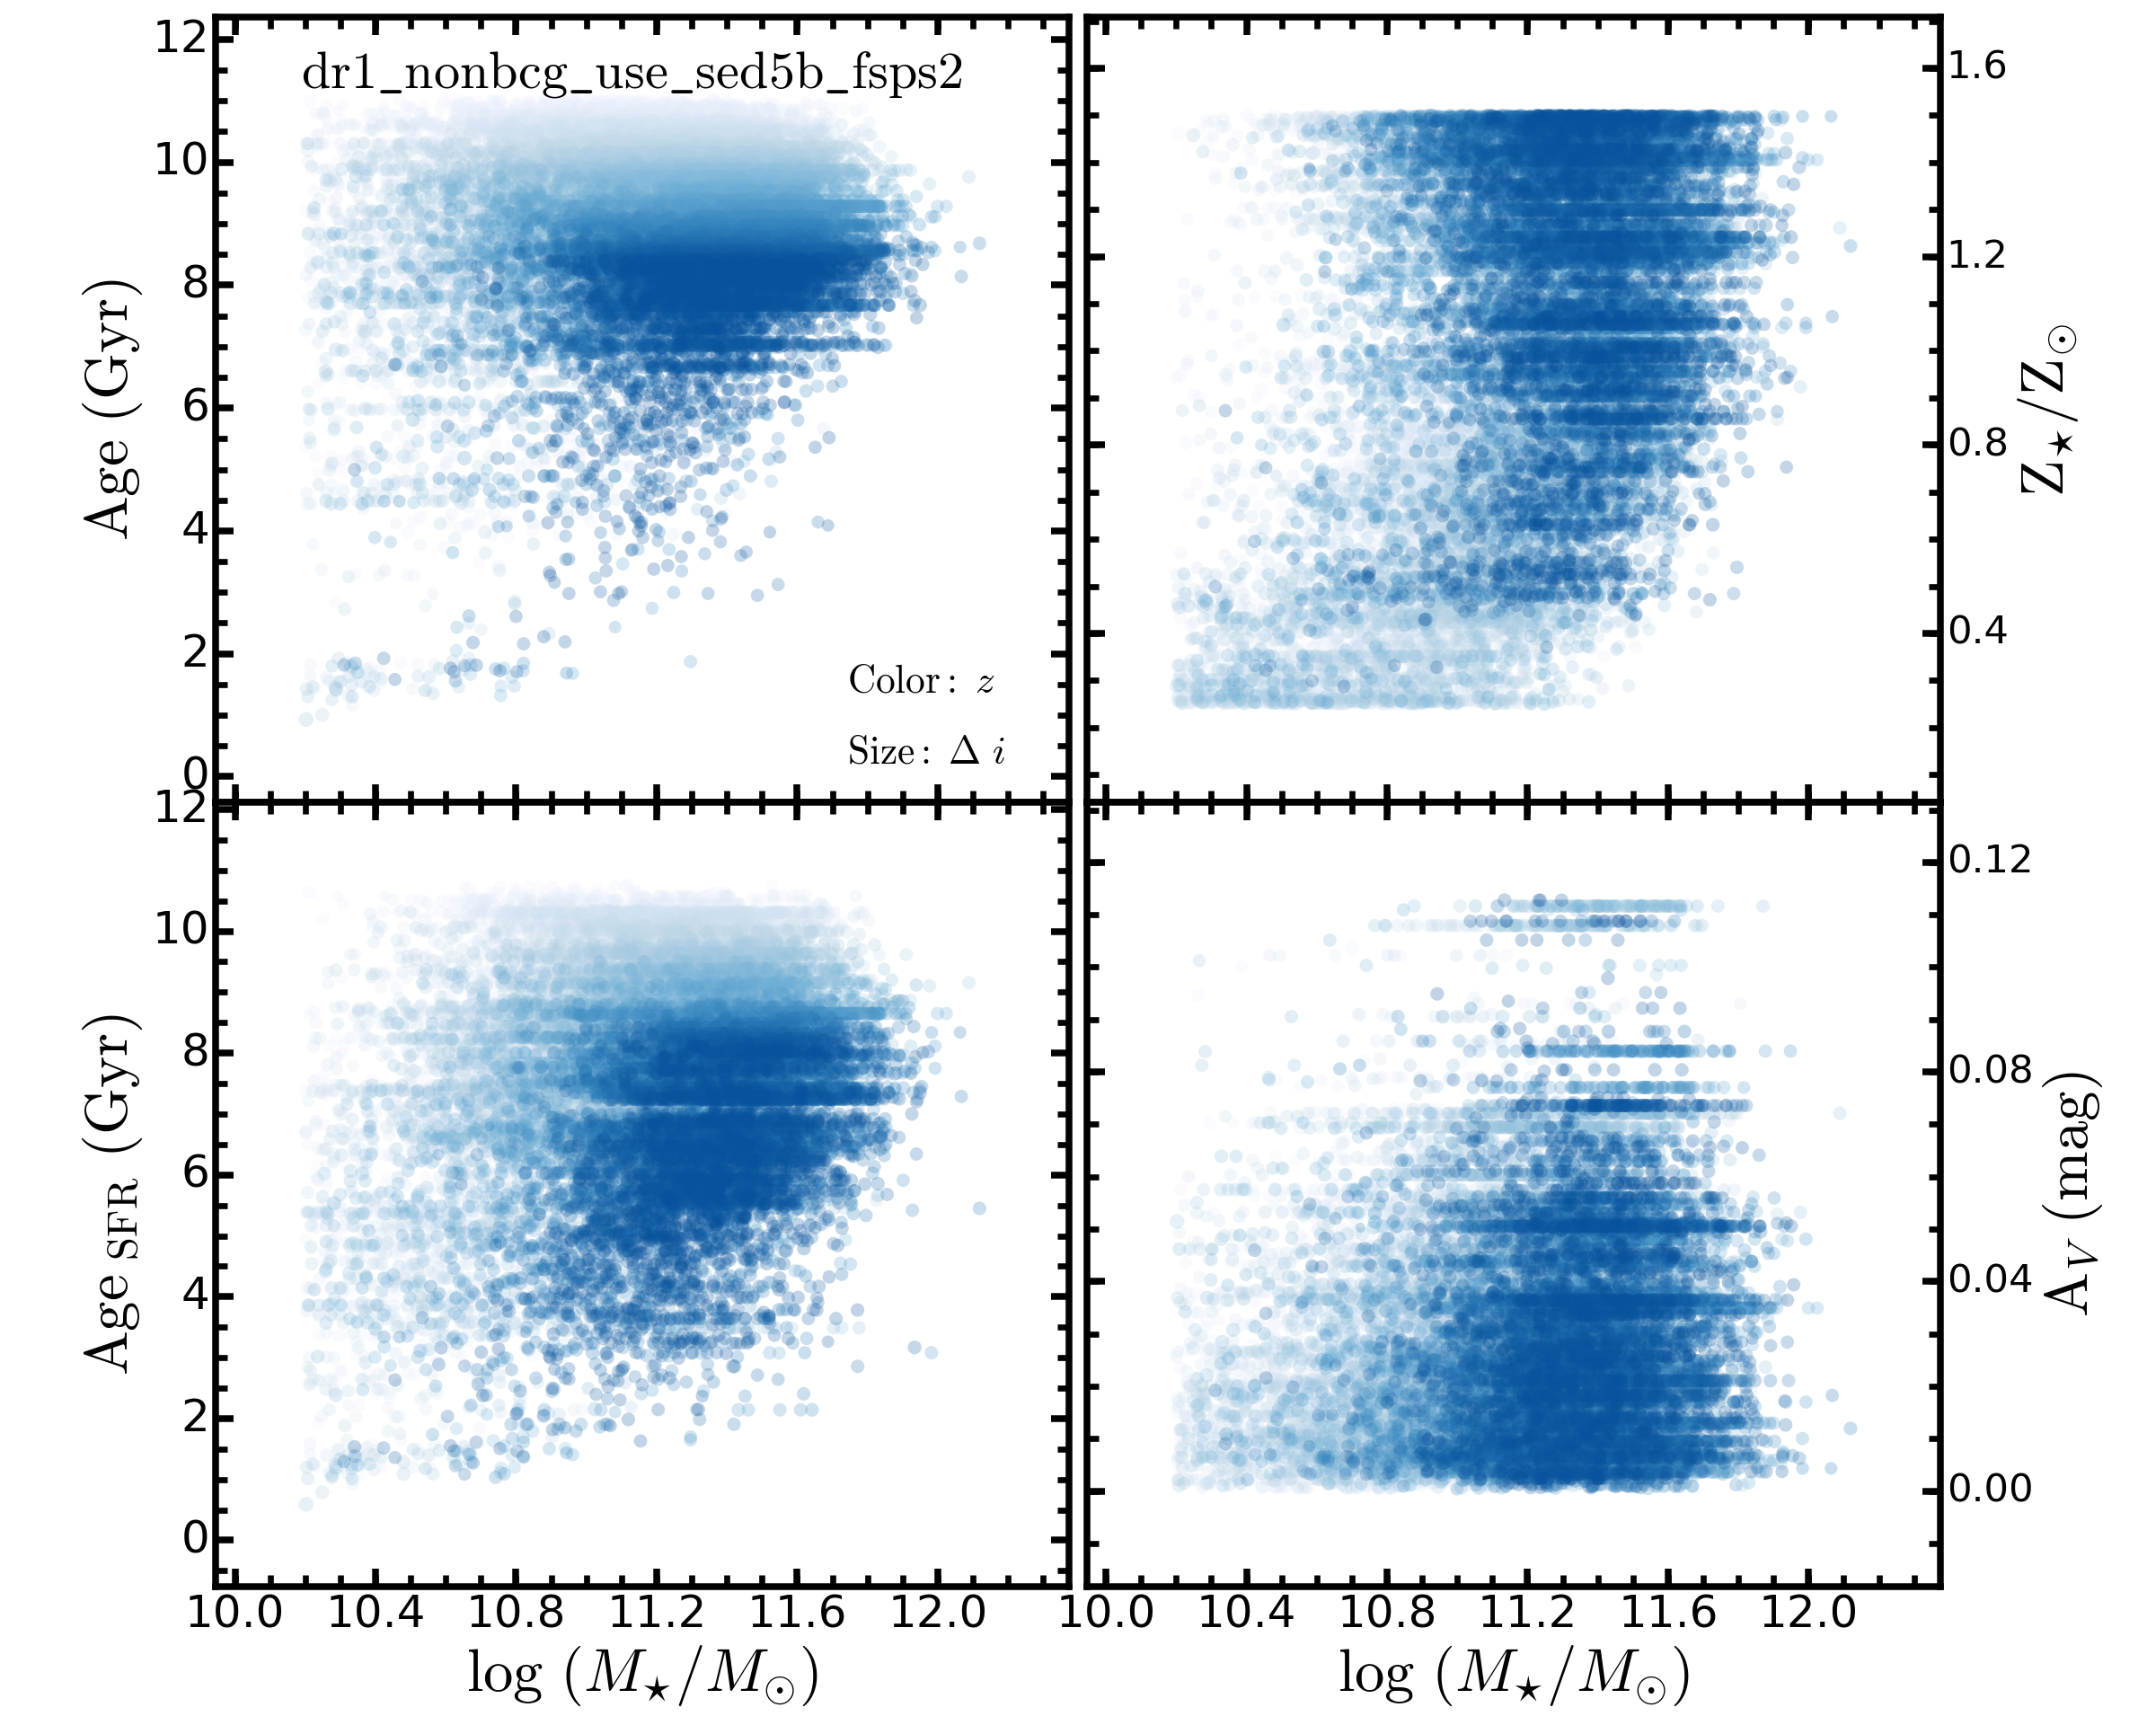
\includegraphics[width=11.5cm]{fig/dr1_nonbcg_use_sed5b_fsps2_logm_plots}
    \caption{Figure.2b\todo{Caption}}\label{figure:2b}
\end{figure}

%%%%%%%%%%%%: End of the File %%%%%%%%%%%%

\end{CJK*}

\clearpage 

%%%%%%%%%%%: Possible Tables %%%%%%%%%%%%%
%\begin{deluxetable}{c ccc cc cc}[b!]
\tabletypesize{\scriptsize}
\tablewidth{0pt}
\tablecolumns{8}
\tablenum{1}
\tablecaption{Average \mden{} Profiles of Massive Galaxies in Different Stellar Mass Bins}
%% ------------------------------------------------------------------------------------ %% 
\tablehead{
    \colhead{Radius} & 
    \multicolumn{3}{c}{[\mden{}]; Combined samples} &
    \multicolumn{2}{c}{[\mden{}]; $M_{\star,100\ \mathrm{kpc}}$-matched} &
    \multicolumn{2}{c}{[\mden{}]; $M_{\star,10\ \mathrm{kpc}}$-matched}
	\vspace{1.4ex}
    %------------------------------------------------------------------------------------%
    \nl 
    \colhead{kpc} & 
    \multicolumn{3}{c}{$\log (M_{\odot}/\mathrm{kpc}^2)$} &
    \multicolumn{2}{c}{$\log (M_{\odot}/\mathrm{kpc}^2)$} &
    \multicolumn{2}{c}{$\log (M_{\odot}/\mathrm{kpc}^2)$}
	\vspace{1.4ex}
    %------------------------------------------------------------------------------------%
    \nl 
    \colhead{} & 
    \colhead{$\log \frac{M_{\star,100\mathrm{kpc}}}{M_{\odot}}\in$[11.4, 11.6]} & 
    \colhead{[11.6, 11.8]} & 
    \colhead{[11.8, 12.0]}\hspace{2.0ex} & 
    \colhead{\texttt{cenHighMh}} & 
    \colhead{\texttt{cenLowMh}} & 
    \colhead{\texttt{cenHighMh}}\hspace{2.0ex} & 
    \colhead{\texttt{cenLowMh}}
    %------------------------------------------------------------------------------------%
	\vspace{1.6ex}
    %------------------------------------------------------------------------------------%
    \nl
    \colhead{    (1)} &
    \colhead{    (2)} &
    \colhead{    (3)} &
    \colhead{    (4)} &
    \colhead{    (5)} &
    \colhead{    (6)} &
    \colhead{    (7)} &
    \colhead{    (8)}
    %------------------------------------------------------------------------------------%
}
%% ------------------------------------------------------------------------------------ %% 
\startdata
%% ------------------------------------------------------------------------------------ %% 

0.0 & $ 9.23\substack{+0.00 \\ -0.00}$ &$ 9.31\substack{+0.00 \\ -0.01}$ &$ 9.32\substack{+0.01 \\ -0.01}$ &$ 9.31\substack{+0.02 \\ -0.02}$ &$ 9.34\substack{+0.01 \\ -0.01}$ &$ 9.31\substack{+0.02 \\ -0.02}$ &$ 9.34\substack{+0.02 \\ -0.02}$ \\
 0.6 & $ 9.20\substack{+0.00 \\ -0.00}$ &$ 9.28\substack{+0.00 \\ -0.01}$ &$ 9.29\substack{+0.01 \\ -0.01}$ &$ 9.27\substack{+0.02 \\ -0.02}$ &$ 9.31\substack{+0.01 \\ -0.01}$ &$ 9.28\substack{+0.02 \\ -0.02}$ &$ 9.31\substack{+0.02 \\ -0.02}$ \\
 1.0 & $ 9.16\substack{+0.00 \\ -0.00}$ &$ 9.24\substack{+0.00 \\ -0.00}$ &$ 9.26\substack{+0.01 \\ -0.01}$ &$ 9.24\substack{+0.02 \\ -0.02}$ &$ 9.27\substack{+0.01 \\ -0.01}$ &$ 9.25\substack{+0.02 \\ -0.02}$ &$ 9.27\substack{+0.02 \\ -0.02}$ \\
 1.4 & $ 9.12\substack{+0.00 \\ -0.00}$ &$ 9.20\substack{+0.00 \\ -0.00}$ &$ 9.23\substack{+0.01 \\ -0.01}$ &$ 9.20\substack{+0.02 \\ -0.02}$ &$ 9.23\substack{+0.01 \\ -0.01}$ &$ 9.21\substack{+0.02 \\ -0.01}$ &$ 9.23\substack{+0.02 \\ -0.01}$ \\
 1.7 & $ 9.06\substack{+0.00 \\ -0.00}$ &$ 9.15\substack{+0.00 \\ -0.00}$ &$ 9.19\substack{+0.01 \\ -0.01}$ &$ 9.15\substack{+0.02 \\ -0.02}$ &$ 9.19\substack{+0.01 \\ -0.01}$ &$ 9.16\substack{+0.01 \\ -0.01}$ &$ 9.18\substack{+0.01 \\ -0.01}$ \\
 2.0 & $ 9.00\substack{+0.00 \\ -0.00}$ &$ 9.10\substack{+0.00 \\ -0.00}$ &$ 9.15\substack{+0.01 \\ -0.01}$ &$ 9.09\substack{+0.01 \\ -0.02}$ &$ 9.13\substack{+0.01 \\ -0.01}$ &$ 9.11\substack{+0.01 \\ -0.01}$ &$ 9.12\substack{+0.01 \\ -0.01}$ \\
 2.4 & $ 8.93\substack{+0.00 \\ -0.00}$ &$ 9.03\substack{+0.00 \\ -0.00}$ &$ 9.09\substack{+0.01 \\ -0.01}$ &$ 9.03\substack{+0.02 \\ -0.02}$ &$ 9.07\substack{+0.01 \\ -0.01}$ &$ 9.05\substack{+0.01 \\ -0.01}$ &$ 9.05\substack{+0.01 \\ -0.01}$ \\
 2.7 & $ 8.87\substack{+0.00 \\ -0.00}$ &$ 8.97\substack{+0.00 \\ -0.00}$ &$ 9.04\substack{+0.01 \\ -0.01}$ &$ 8.97\substack{+0.01 \\ -0.01}$ &$ 9.01\substack{+0.01 \\ -0.01}$ &$ 9.00\substack{+0.01 \\ -0.01}$ &$ 8.99\substack{+0.01 \\ -0.01}$ \\
 3.0 & $ 8.80\substack{+0.00 \\ -0.00}$ &$ 8.90\substack{+0.00 \\ -0.00}$ &$ 8.98\substack{+0.01 \\ -0.01}$ &$ 8.90\substack{+0.01 \\ -0.01}$ &$ 8.95\substack{+0.01 \\ -0.01}$ &$ 8.93\substack{+0.01 \\ -0.01}$ &$ 8.92\substack{+0.01 \\ -0.01}$ \\
 3.4 & $ 8.72\substack{+0.00 \\ -0.00}$ &$ 8.83\substack{+0.00 \\ -0.00}$ &$ 8.92\substack{+0.01 \\ -0.01}$ &$ 8.83\substack{+0.01 \\ -0.01}$ &$ 8.88\substack{+0.01 \\ -0.01}$ &$ 8.86\substack{+0.01 \\ -0.01}$ &$ 8.85\substack{+0.01 \\ -0.01}$ \\
 3.7 & $ 8.66\substack{+0.00 \\ -0.00}$ &$ 8.78\substack{+0.00 \\ -0.00}$ &$ 8.87\substack{+0.01 \\ -0.01}$ &$ 8.78\substack{+0.01 \\ -0.01}$ &$ 8.83\substack{+0.01 \\ -0.01}$ &$ 8.81\substack{+0.01 \\ -0.01}$ &$ 8.79\substack{+0.01 \\ -0.01}$ \\
 4.1 & $ 8.60\substack{+0.00 \\ -0.00}$ &$ 8.72\substack{+0.00 \\ -0.00}$ &$ 8.82\substack{+0.01 \\ -0.01}$ &$ 8.72\substack{+0.01 \\ -0.01}$ &$ 8.77\substack{+0.01 \\ -0.01}$ &$ 8.76\substack{+0.01 \\ -0.01}$ &$ 8.73\substack{+0.01 \\ -0.01}$ \\
 4.4 & $ 8.54\substack{+0.00 \\ -0.00}$ &$ 8.66\substack{+0.00 \\ -0.00}$ &$ 8.77\substack{+0.01 \\ -0.01}$ &$ 8.66\substack{+0.01 \\ -0.01}$ &$ 8.72\substack{+0.01 \\ -0.01}$ &$ 8.70\substack{+0.01 \\ -0.01}$ &$ 8.67\substack{+0.01 \\ -0.01}$ \\
 4.8 & $ 8.48\substack{+0.00 \\ -0.00}$ &$ 8.60\substack{+0.00 \\ -0.00}$ &$ 8.71\substack{+0.01 \\ -0.01}$ &$ 8.60\substack{+0.01 \\ -0.01}$ &$ 8.66\substack{+0.01 \\ -0.01}$ &$ 8.65\substack{+0.01 \\ -0.01}$ &$ 8.61\substack{+0.01 \\ -0.01}$ \\
 6.2 & $ 8.26\substack{+0.00 \\ -0.00}$ &$ 8.40\substack{+0.00 \\ -0.00}$ &$ 8.53\substack{+0.01 \\ -0.01}$ &$ 8.41\substack{+0.01 \\ -0.01}$ &$ 8.46\substack{+0.01 \\ -0.01}$ &$ 8.46\substack{+0.02 \\ -0.02}$ &$ 8.40\substack{+0.02 \\ -0.02}$ \\
 7.6 & $ 8.09\substack{+0.00 \\ -0.00}$ &$ 8.24\substack{+0.00 \\ -0.00}$ &$ 8.39\substack{+0.01 \\ -0.01}$ &$ 8.27\substack{+0.01 \\ -0.01}$ &$ 8.31\substack{+0.01 \\ -0.01}$ &$ 8.31\substack{+0.02 \\ -0.02}$ &$ 8.23\substack{+0.02 \\ -0.02}$ \\
 9.0 & $ 7.95\substack{+0.00 \\ -0.00}$ &$ 8.10\substack{+0.00 \\ -0.00}$ &$ 8.27\substack{+0.01 \\ -0.01}$ &$ 8.14\substack{+0.02 \\ -0.02}$ &$ 8.18\substack{+0.01 \\ -0.01}$ &$ 8.19\substack{+0.02 \\ -0.02}$ &$ 8.09\substack{+0.02 \\ -0.02}$ \\
10.3 & $ 7.82\substack{+0.00 \\ -0.00}$ &$ 7.99\substack{+0.00 \\ -0.00}$ &$ 8.16\substack{+0.01 \\ -0.01}$ &$ 8.03\substack{+0.02 \\ -0.01}$ &$ 8.06\substack{+0.01 \\ -0.01}$ &$ 8.09\substack{+0.02 \\ -0.02}$ &$ 7.97\substack{+0.02 \\ -0.02}$ \\
11.7 & $ 7.70\substack{+0.00 \\ -0.00}$ &$ 7.88\substack{+0.00 \\ -0.00}$ &$ 8.06\substack{+0.01 \\ -0.01}$ &$ 7.93\substack{+0.02 \\ -0.02}$ &$ 7.96\substack{+0.01 \\ -0.01}$ &$ 7.99\substack{+0.02 \\ -0.02}$ &$ 7.85\substack{+0.02 \\ -0.02}$ \\
13.0 & $ 7.60\substack{+0.00 \\ -0.00}$ &$ 7.78\substack{+0.00 \\ -0.00}$ &$ 7.98\substack{+0.01 \\ -0.01}$ &$ 7.85\substack{+0.02 \\ -0.02}$ &$ 7.87\substack{+0.01 \\ -0.01}$ &$ 7.90\substack{+0.02 \\ -0.02}$ &$ 7.75\substack{+0.02 \\ -0.02}$ \\
14.5 & $ 7.50\substack{+0.00 \\ -0.00}$ &$ 7.69\substack{+0.00 \\ -0.00}$ &$ 7.90\substack{+0.01 \\ -0.01}$ &$ 7.76\substack{+0.02 \\ -0.02}$ &$ 7.78\substack{+0.01 \\ -0.01}$ &$ 7.82\substack{+0.02 \\ -0.02}$ &$ 7.65\substack{+0.02 \\ -0.02}$ \\
16.0 & $ 7.39\substack{+0.00 \\ -0.00}$ &$ 7.60\substack{+0.00 \\ -0.00}$ &$ 7.82\substack{+0.01 \\ -0.01}$ &$ 7.68\substack{+0.02 \\ -0.02}$ &$ 7.69\substack{+0.01 \\ -0.01}$ &$ 7.74\substack{+0.02 \\ -0.03}$ &$ 7.56\substack{+0.02 \\ -0.03}$ \\
17.3 & $ 7.31\substack{+0.00 \\ -0.00}$ &$ 7.52\substack{+0.00 \\ -0.00}$ &$ 7.76\substack{+0.01 \\ -0.01}$ &$ 7.61\substack{+0.02 \\ -0.02}$ &$ 7.62\substack{+0.01 \\ -0.01}$ &$ 7.67\substack{+0.03 \\ -0.03}$ &$ 7.48\substack{+0.03 \\ -0.03}$ \\
18.7 & $ 7.23\substack{+0.00 \\ -0.00}$ &$ 7.45\substack{+0.00 \\ -0.00}$ &$ 7.69\substack{+0.01 \\ -0.01}$ &$ 7.55\substack{+0.02 \\ -0.02}$ &$ 7.55\substack{+0.01 \\ -0.01}$ &$ 7.61\substack{+0.03 \\ -0.03}$ &$ 7.40\substack{+0.03 \\ -0.03}$ \\
22.6 & $ 7.02\substack{+0.00 \\ -0.00}$ &$ 7.27\substack{+0.00 \\ -0.00}$ &$ 7.54\substack{+0.01 \\ -0.01}$ &$ 7.38\substack{+0.02 \\ -0.02}$ &$ 7.37\substack{+0.01 \\ -0.01}$ &$ 7.45\substack{+0.03 \\ -0.03}$ &$ 7.21\substack{+0.03 \\ -0.03}$ \\
26.1 & $ 6.86\substack{+0.00 \\ -0.00}$ &$ 7.12\substack{+0.00 \\ -0.00}$ &$ 7.41\substack{+0.01 \\ -0.01}$ &$ 7.25\substack{+0.02 \\ -0.02}$ &$ 7.24\substack{+0.01 \\ -0.01}$ &$ 7.32\substack{+0.03 \\ -0.03}$ &$ 7.05\substack{+0.03 \\ -0.03}$ \\
30.0 & $ 6.70\substack{+0.00 \\ -0.00}$ &$ 6.98\substack{+0.00 \\ -0.00}$ &$ 7.29\substack{+0.01 \\ -0.01}$ &$ 7.13\substack{+0.03 \\ -0.02}$ &$ 7.10\substack{+0.01 \\ -0.01}$ &$ 7.20\substack{+0.03 \\ -0.04}$ &$ 6.90\substack{+0.03 \\ -0.04}$ \\
33.7 & $ 6.55\substack{+0.00 \\ -0.00}$ &$ 6.85\substack{+0.01 \\ -0.01}$ &$ 7.18\substack{+0.01 \\ -0.01}$ &$ 7.01\substack{+0.03 \\ -0.03}$ &$ 6.98\substack{+0.01 \\ -0.01}$ &$ 7.09\substack{+0.03 \\ -0.03}$ &$ 6.76\substack{+0.03 \\ -0.03}$ \\
37.8 & $ 6.41\substack{+0.00 \\ -0.00}$ &$ 6.72\substack{+0.01 \\ -0.01}$ &$ 7.07\substack{+0.01 \\ -0.01}$ &$ 6.90\substack{+0.03 \\ -0.03}$ &$ 6.85\substack{+0.01 \\ -0.01}$ &$ 6.98\substack{+0.04 \\ -0.04}$ &$ 6.63\substack{+0.04 \\ -0.04}$ \\
41.6 & $ 6.29\substack{+0.01 \\ -0.01}$ &$ 6.61\substack{+0.01 \\ -0.01}$ &$ 6.98\substack{+0.01 \\ -0.01}$ &$ 6.81\substack{+0.03 \\ -0.03}$ &$ 6.75\substack{+0.01 \\ -0.01}$ &$ 6.89\substack{+0.04 \\ -0.04}$ &$ 6.51\substack{+0.04 \\ -0.04}$ \\
45.7 & $ 6.17\substack{+0.01 \\ -0.01}$ &$ 6.50\substack{+0.01 \\ -0.01}$ &$ 6.88\substack{+0.01 \\ -0.01}$ &$ 6.71\substack{+0.03 \\ -0.03}$ &$ 6.64\substack{+0.01 \\ -0.01}$ &$ 6.79\substack{+0.04 \\ -0.04}$ &$ 6.39\substack{+0.04 \\ -0.04}$ \\
49.3 & $ 6.07\substack{+0.01 \\ -0.01}$ &$ 6.41\substack{+0.01 \\ -0.01}$ &$ 6.80\substack{+0.01 \\ -0.02}$ &$ 6.62\substack{+0.03 \\ -0.03}$ &$ 6.56\substack{+0.01 \\ -0.01}$ &$ 6.70\substack{+0.04 \\ -0.04}$ &$ 6.30\substack{+0.04 \\ -0.04}$ \\
53.1 & $ 5.98\substack{+0.01 \\ -0.01}$ &$ 6.33\substack{+0.01 \\ -0.01}$ &$ 6.71\substack{+0.02 \\ -0.02}$ &$ 6.55\substack{+0.03 \\ -0.03}$ &$ 6.46\substack{+0.01 \\ -0.01}$ &$ 6.64\substack{+0.04 \\ -0.04}$ &$ 6.21\substack{+0.04 \\ -0.04}$ \\
57.2 & $ 5.88\substack{+0.01 \\ -0.01}$ &$ 6.24\substack{+0.01 \\ -0.01}$ &$ 6.63\substack{+0.02 \\ -0.02}$ &$ 6.47\substack{+0.04 \\ -0.04}$ &$ 6.37\substack{+0.01 \\ -0.01}$ &$ 6.56\substack{+0.04 \\ -0.04}$ &$ 6.11\substack{+0.04 \\ -0.04}$ \\
61.5 & $ 5.79\substack{+0.01 \\ -0.01}$ &$ 6.15\substack{+0.01 \\ -0.01}$ &$ 6.55\substack{+0.02 \\ -0.02}$ &$ 6.39\substack{+0.04 \\ -0.04}$ &$ 6.29\substack{+0.01 \\ -0.01}$ &$ 6.49\substack{+0.04 \\ -0.04}$ &$ 6.03\substack{+0.04 \\ -0.04}$ \\
66.0 & $ 5.70\substack{+0.01 \\ -0.01}$ &$ 6.05\substack{+0.01 \\ -0.01}$ &$ 6.47\substack{+0.02 \\ -0.02}$ &$ 6.32\substack{+0.04 \\ -0.04}$ &$ 6.20\substack{+0.01 \\ -0.01}$ &$ 6.37\substack{+0.05 \\ -0.06}$ &$ 5.94\substack{+0.05 \\ -0.06}$ \\
69.8 & $ 5.64\substack{+0.01 \\ -0.01}$ &$ 5.98\substack{+0.01 \\ -0.01}$ &$ 6.40\substack{+0.02 \\ -0.02}$ &$ 6.25\substack{+0.04 \\ -0.04}$ &$ 6.12\substack{+0.02 \\ -0.01}$ &$ 6.35\substack{+0.04 \\ -0.05}$ &$ 5.87\substack{+0.04 \\ -0.05}$ \\
74.7 & $ 5.56\substack{+0.01 \\ -0.01}$ &$ 5.89\substack{+0.01 \\ -0.01}$ &$ 6.32\substack{+0.02 \\ -0.02}$ &$ 6.18\substack{+0.04 \\ -0.04}$ &$ 6.04\substack{+0.02 \\ -0.02}$ &$ 6.28\substack{+0.05 \\ -0.05}$ &$ 5.79\substack{+0.05 \\ -0.05}$ \\
79.9 & $ 5.49\substack{+0.01 \\ -0.01}$ &$ 5.81\substack{+0.01 \\ -0.01}$ &$ 6.24\substack{+0.02 \\ -0.02}$ &$ 6.12\substack{+0.04 \\ -0.04}$ &$ 5.96\substack{+0.02 \\ -0.02}$ &$ 6.20\substack{+0.05 \\ -0.06}$ &$ 5.72\substack{+0.05 \\ -0.06}$ \\
84.3 & $ 5.43\substack{+0.01 \\ -0.01}$ &$ 5.74\substack{+0.01 \\ -0.01}$ &$ 6.18\substack{+0.02 \\ -0.02}$ &$ 6.05\substack{+0.04 \\ -0.05}$ &$ 5.89\substack{+0.02 \\ -0.02}$ &$ 6.16\substack{+0.05 \\ -0.05}$ &$ 5.65\substack{+0.05 \\ -0.05}$ \\
88.8 & $ 5.38\substack{+0.01 \\ -0.01}$ &$ 5.67\substack{+0.01 \\ -0.01}$ &$ 6.11\substack{+0.02 \\ -0.02}$ &$ 5.99\substack{+0.05 \\ -0.06}$ &$ 5.81\substack{+0.02 \\ -0.02}$ &$ 6.08\substack{+0.05 \\ -0.06}$ &$ 5.58\substack{+0.05 \\ -0.06}$ \\
97.2 & $ 5.29\substack{+0.01 \\ -0.01}$ &$ 5.56\substack{+0.01 \\ -0.01}$ &$ 5.98\substack{+0.02 \\ -0.02}$ &$ 5.92\substack{+0.04 \\ -0.04}$ &$ 5.69\substack{+0.02 \\ -0.02}$ &$ 5.99\substack{+0.05 \\ -0.05}$ &$ 5.47\substack{+0.05 \\ -0.05}$ \\
103.6 & $ 5.21\substack{+0.01 \\ -0.01}$ &$ 5.49\substack{+0.01 \\ -0.01}$ &$ 5.89\substack{+0.03 \\ -0.03}$ &$ 5.84\substack{+0.05 \\ -0.05}$ &$ 5.62\substack{+0.02 \\ -0.02}$ &$ 5.94\substack{+0.05 \\ -0.05}$ &$ 5.39\substack{+0.05 \\ -0.05}$ \\
111.6 & $ 5.14\substack{+0.01 \\ -0.01}$ &$ 5.40\substack{+0.01 \\ -0.01}$ &$ 5.79\substack{+0.03 \\ -0.03}$ &$ 5.78\substack{+0.05 \\ -0.05}$ &$ 5.54\substack{+0.02 \\ -0.02}$ &$ 5.87\substack{+0.05 \\ -0.05}$ &$ 5.32\substack{+0.05 \\ -0.05}$ \\
117.2 & $ 5.10\substack{+0.01 \\ -0.01}$ &$ 5.36\substack{+0.01 \\ -0.01}$ &$ 5.72\substack{+0.03 \\ -0.03}$ &$ 5.72\substack{+0.05 \\ -0.05}$ &$ 5.47\substack{+0.02 \\ -0.02}$ &$ 5.82\substack{+0.05 \\ -0.05}$ &$ 5.29\substack{+0.05 \\ -0.05}$ \\
129.0 & $ 5.00\substack{+0.01 \\ -0.01}$ &$ 5.25\substack{+0.02 \\ -0.02}$ &$ 5.61\substack{+0.03 \\ -0.03}$ &$ 5.64\substack{+0.05 \\ -0.05}$ &$ 5.36\substack{+0.02 \\ -0.02}$ &$ 5.74\substack{+0.05 \\ -0.05}$ &$ 5.21\substack{+0.05 \\ -0.05}$ \\
141.7 & $ 4.89\substack{+0.02 \\ -0.02}$ &$ 5.13\substack{+0.02 \\ -0.02}$ &$ 5.49\substack{+0.03 \\ -0.03}$ &$ 5.58\substack{+0.05 \\ -0.05}$ &$ 5.23\substack{+0.03 \\ -0.03}$ &$ 5.66\substack{+0.05 \\ -0.05}$ &$ 5.09\substack{+0.05 \\ -0.05}$ \\
146.7 & $ 4.85\substack{+0.02 \\ -0.02}$ &$ 5.10\substack{+0.02 \\ -0.02}$ &$ 5.46\substack{+0.03 \\ -0.03}$ &$ 5.51\substack{+0.06 \\ -0.06}$ &$ 5.19\substack{+0.03 \\ -0.03}$ &$ 5.61\substack{+0.05 \\ -0.05}$ &$ 5.03\substack{+0.05 \\ -0.05}$ \\

%%------------------------------------------------------------------------------------ %% 
\enddata
%% ------------------------------------------------------------------------------------ %% 
\tablecomments{
    Average \mden{} profiles of massive \rbcg{} and \nbcg{} galaxies in different
    samples:\\ 
    Col.~(1) Radius along the major axis in kpc.\\
    Col.~(2) Average \mden{} profile for galaxies with 
        $11.4 \leq$\logmtot$< 11.6$ in the combined samples of \rbcg{} and \nbcg{}
        galaxies. \\ 
    Col.~(3) Average \mden{} profile of combined samples in the mass bin of 
        $11.6 \leq$\logmtot$< 11.8$. \\ 
    Col.~(4) Average \mden{} profile of combined samples in the mass bin of 
        $11.8 \leq$\logmtot$< 12.0$. \\ 
    Col.~(5) and Col.~(6) are the average \mden{} profiles of \rbcg{} and \nbcg{} galaxies
        in the \mtot{}-matched samples within $11.6 \leq$\logmtot{}$< 11.9$. \\ 
    Col.~(7) and Col.~(8) are the average \mden{} profiles of \rbcg{} and \nbcg{} galaxies 
        in the \minn{}-matched samples within $11.2 \leq$\logmtot{}$< 11.6$. \\ 
    The upper and lower uncertainties of these average profiles vial bootstrap-resampling 
    method are also displayed.
}
\label{tab:prof}
\end{deluxetable}


\label{lastpage}
\end{document}